\documentclass[12pt,a4paper]{report}
\usepackage{listings}
\usepackage{xcolor} 
\usepackage{indentfirst}
\usepackage{float}
\usepackage[utf8]{inputenc}
\usepackage[T1]{fontenc}
\usepackage[brazil]{babel}
\usepackage{graphicx}
\usepackage{amsmath, amssymb}
\usepackage{hyperref}
\usepackage{caption}
\captionsetup{labelformat=empty}

% Margens
\usepackage[a4paper,margin=2.5cm]{geometry}

\setlength{\parindent}{1.25cm}
\setlength{\parskip}{0.2cm}
\lstset{
    inputencoding=utf8,     
    extendedchars=true,     
    literate=
    {á}{{\'a}}1 {ã}{{\~a}}1 {â}{{\^a}}1 {à}{{\`a}}1
    {é}{{\'e}}1 {ê}{{\^e}}1 {í}{{\'i}}1 {ó}{{\'o}}1
    {ô}{{\^o}}1 {õ}{{\~o}}1 {ú}{{\'u}}1 {ç}{{\c{c}}}1
    {Á}{{\'A}}1 {Ã}{{\~A}}1 {Â}{{\^A}}1 {À}{{\`A}}1
    {É}{{\'E}}1 {Ê}{{\^E}}1 {Í}{{\'I}}1 {Ó}{{\'O}}1
    {Ô}{{\^O}}1 {Õ}{{\~O}}1 {Ú}{{\'U}}1 {Ç}{{\c{C}}}1,
    basicstyle=\scriptsize\ttfamily,     
    numbers=left,                   
    numberstyle=\tiny\color{gray}, 
    stepnumber=1,                   
    breaklines=true,               
    frame=single,                  
    captionpos=b,                  
    keywordstyle=\color{blue},     
    commentstyle=\color{gray},     
    stringstyle=\color{orange},    
}
\makeatletter
\renewcommand{\@makechapterhead}[1]{%
  \vspace*{5pt} 
  {\parindent \z@
    \normalfont\Large\bfseries #1\par\nobreak
    \vskip 15pt 
  }}
\makeatother
\setcounter{secnumdepth}{0}

\begin{document}
\frenchspacing

%-----------------------------
% CAPA
%-----------------------------
\begin{titlepage}
\begin{figure}[h!] 
    \centering
    
\includegraphics[width=0.2\textwidth]{logo.png}
    \label{fig:minha-figura}
\end{figure}
    \begin{center}
        \large
        \textbf {FACULDADE CESAR SCHOOL}\\
        CURSO DE GRADUAÇÃO EM CIÊNCIA DA COMPUTAÇÃO
        
        \vfill
        
        \Huge
        \textbf{Relatório do Projeto de Banco de Dados}
        
        \vfill
        
        \large
        \textbf {Ana Clara Gomes da Silva\\
        Gabriel Melo Calvacanti de Albuquerque \\
        Julia Sales Novais\\
        Sophia de Araujo Gallindo Pinto}
        
        
        \vfill
        
        \normalsize
        Recife \\
        MAIO/2025
    \end{center}
\end{titlepage}

%-----------------------------
% SUMÁRIO
%-----------------------------
\newpage
\tableofcontents
\newpage

%-----------------------------
% CAPÍTULOS
%-----------------------------
\renewcommand{\chaptername}{}  
\renewcommand{\thechapter}{}   

\chapter{1. Introdução}

O projeto foi desenvolvido para a disciplina de Modelagem e Projeto de Banco de Dados e consiste em uma aplicação web construída com Spring Boot (back-end) e React (front-end). A proposta é baseada no RPG de mesa "Ordem Paranormal", um universo fictício de investigação sobrenatural criado pelo streamer brasileiro Rafael Lange (Também conhecido como Cellbit).

O objetivo desse projeto é criar um sistema ficticio de gerenciamento e alocação de equipes em missões para investigar e conter ameaças paranormais. Para isso, foi utilizada a ferramenta MySQL para possilitar a permanência de dados na aplicação.

O repositório do projeto pode ser encontrado aqui: \href{https://github.com/Taverna-Hub/OrdemParanormalBD}{https://github.com/Taverna-Hub/OrdemParanormalBD}

\chapter{2. Mini Mundo}
\begin{itemize}
    \item \textbf {Ordo Realitas:} 
    
    A Ordo Realitas é uma organização secreta criada com o objetivo de investigar e combater manifestações paranormais, protegendo a Realidade de ameaças vindas do Outro Lado. Fundada em um período desconhecido da história, a organização opera de forma discreta e estruturada, garantindo que seus agentes tenham os recursos necessários para enfrentar o desconhecido. 
    
    Sua infraestrutura é complexa e bem distribuída, contando com bases operacionais altamente equipadas, tecnologia de ponta e um sistema de segurança avançado para proteger seus arquivos e instalações.

    
    \item \textbf {Ordo Realitas e seu Comando:}
    
    A liderança da Ordo Realistas está sob a responsabilidade de Veríssimo, o título concedido ao mais alto comandante da organização. Ele é o responsável por tomar as decisões estratégicas, organizar as operações e distribuir missões às equipes de campo. Além da base principal, a Ordo Realitas conta com infraestrutura auxiliar espalhada estrategicamente, garantindo maior alcance e eficiência no cumprimento de suas tarefas.
    
    \item \textbf {Os Agentes:} 
    
    Os agentes trabalham no QG e são indivíduos altamente treinados para lidar com fenômenos paranormais. Cada agente recebe um código de identificação e têm nome completo, telefone e data de nascimento, especialidade (podendo ser Ocultista, Especialista e Combatente)  e nível de exposição ao paranormal (NEX), que aumenta a cada missão. Além disso, eles ainda têm uma patente (podendo ser recruta, veterano ou elite) dentro da Ordo Realitas. O histórico de missão de cada agente é documentado. Caso um agente tenha se ligado a um elemento (ao atingir 50% de exposição), ele recebe o status de transcendido e se torna capaz de utilizar rituais. Os agentes podem se aposentar, não podendo mais ser enviados em missões.
    
    Para acessar o sistema, o agente que é Veríssimo precisa de um login e senha.
    
    \item \textbf {As Equipes:}
    
    Para garantir eficiência no combate ao paranormal, os agentes são organizados em equipes operacionais. Cada equipe possui um nome próprio. Dependendo da sua especialização, uma equipe pode focar em investigação, combate ou suporte. O histórico de missões de cada equipe é mantido nos arquivos da organização.
    Cada equipe é responsável por uma missão. Um histórico de quais agentes passaram por aquela equipe é mantido, juntamente com sua data de ingresso e data de saída.

    
    \item \textbf {Missões e Ameaças:}
    
    O Veríssimo é responsável por abrir missões, as missões conduzidas seguem um rigoroso protocolo, sendo registradas com um código de identificação específico para cada caso e um título da missão, a localização do fenômeno (tendo as mesmas informações de localização do QG), os objetivos da missão e as evidências coletadas.
    
    Uma missão pode ter mais de uma equipe envolvida O nível de risco envolvido em cada missão é cuidadosamente avaliado, garantindo que os agentes estejam preparados para lidar com as ameaças encontradas, cada missão é primeiramente associada a uma ou mais ameaças a serem neutralizadas. Em seguida, essa mesma missão é atribuída a uma ou mais equipes, essa atribuição recebe data de alocação e desalocação (caso a equipe seja trocada durante a missão), e podendo efetivar na neutralização da(s) ameaça(s) pela equipe envolvida.
    
    Ao final da missão, o status da missão pode ser classificado como: aberto, concluído ou arquivado, dependendo dos resultados obtidos.
    
    As ameaças são divididas em duas categorias principais: entidades paranormais e organização. Cada ameaça é identificada por um código, podendo ter um ou mais nomes e possui uma descrição detalhada de suas características e comportamento. Seu nível de periculosidade é classificado conforme seu impacto na realidade. Além disso, um histórico de ocorrências registra todos os encontros anteriores com a ameaça, elas também estarão associadas a um ou mais dos cinco elementos fundamentais: medo, sangue, morte, conhecimento ou energia. 
    
    Caso a ameaça seja entidade paranormal, elas têm uma ou mais habilidades e podem possuir um Enigma a ser decifrado, que pode enfraquecer ou derrotar a entidade. 
    
    Caso seja uma ameaça de organização, elas são formadas por um ou mais integrantes, esses integrantes podem ou não possuir rituais, possuem nome e papel dentro da organização (podendo ser Líder, Pesquisador, Ocultista ou Simpatizante).
    
    Nesse contexto, é evidente a necessidade de relação entre, as equipes, missão, e Ameaça.

    
    \item \textbf {Evidências e Elementos Paranormais:}
    
    Durante as missões, as equipes coletam evidências. Cada evidência recebe um código de identificação oficial e é catalogada com uma descrição detalhada, incluindo a origem dela, sua possível relação com a ameaça investigada e nível de estabilidade paranormal( podendo ser Estável, Volátil, Perigoso ou Contido). Todas as evidências são vinculadas à missão correspondente, e servem de guia para a resolução do enigma da ameaça, caso a mesma seja uma entidade paranormal.
    
    Os elementos paranormais são manifestações diretas das forças do Outro Lado. Cada elemento recebe um nome único e uma descrição detalhada, indicando sua natureza e efeitos observados. O histórico de ocorrências desses elementos é mantido nos registros da organização por meio das ameaças registradas. Cada elemento também é forte e fraco contra um dos outros elementos, sendo o ‘Medo’ o elemento neutro.
	Morte é forte contra Sangue
	Sangue é forte contra conhecimento
	Conhecimento é forte contra energia 
	Energia é forte contra morte

    
    \item \textbf {Rituais:}
    
    Os rituais são práticas ocultistas utilizadas experientes da Ordo Realitas. Cada ritual possui um nome e uma descrição detalhada de seus efeitos, além de uma lista de requisitos necessários para sua realização e uma lista de riscos associados, e um elemento ao qual o ritual está associado.

    
    \item \textbf {O Quartel-General (QG):}
    
    O QG da Ordo Realitas é o centro de operações da organização, onde agentes treinam, investigam casos e armazenam evidências. Cada base operacional recebe um codinome, localização(contendo: rua, número, bairro, cep, estado e cidade), contém quantidade de salas e nível de segurança.
    
    A segurança e confidencialidade da base é uma das prioridades da Ordo Realitas, sendo classificada com uma nota de 0.0 a 10.0.
    
    Cada QG é comandado por um agente, denominado Veríssimo, Quando um novo agente assume, ele muda o seu nome para Sr Veríssimo, e passa a administrar o QG.


\end{itemize}


\chapter{3. Modelos}

\section{3.1 Modelo Conceitual}
\begin{figure}[ht!]
    \centering
    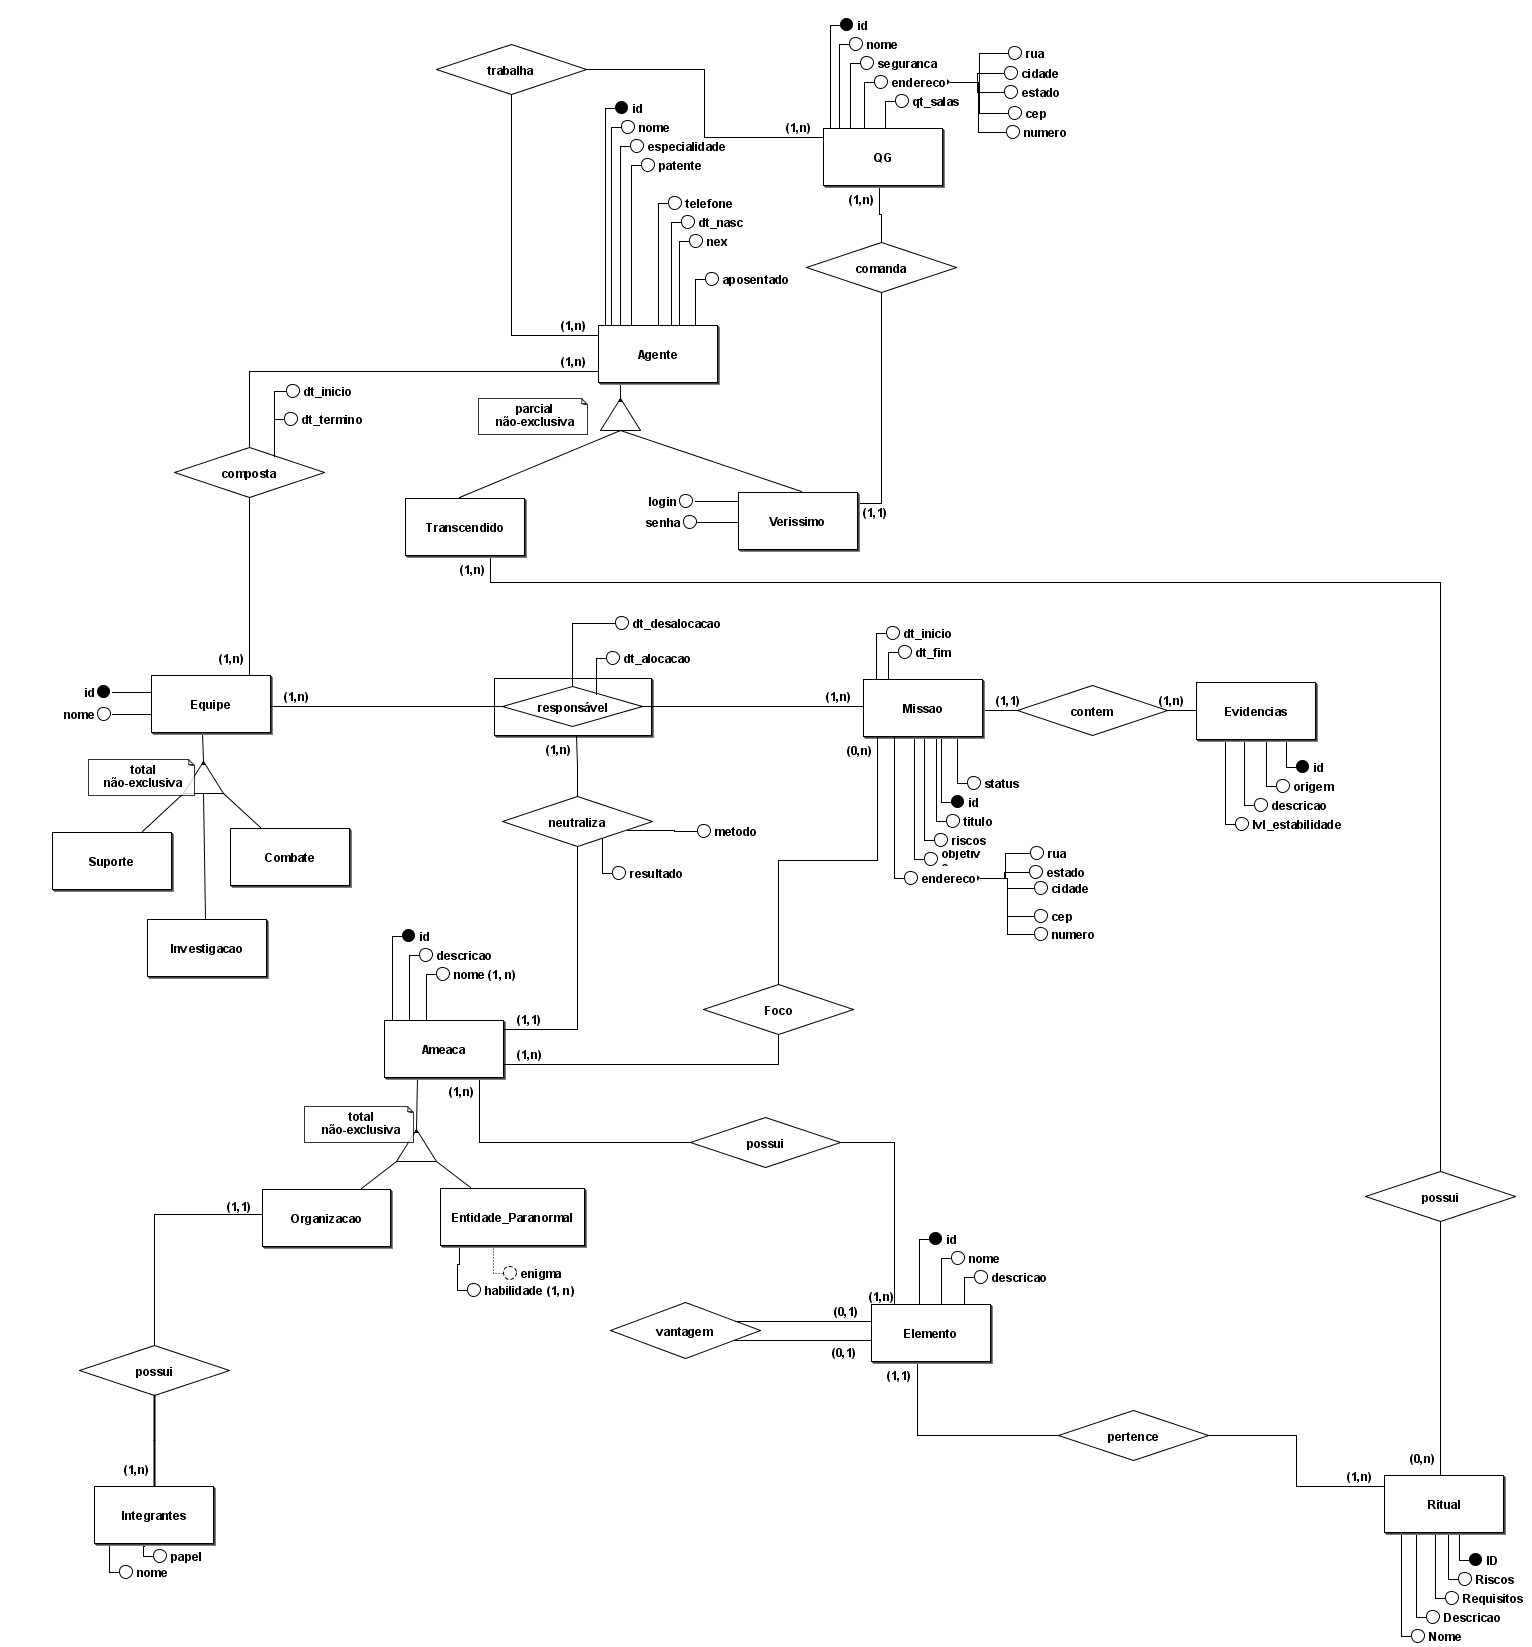
\includegraphics[width=0.95\textwidth]{Conceitual-ordem.png}
    \label{fig:conceitual-ordem}
\end{figure}

Esse Modelo foi criado a partir da análise do Mini Mundo e foi utilizado para a primeira visualização do banco de dados a ser criado e as seguintes informações foram observadas e concluídas:


\begin{itemize}
  \item \textbf{Entidades:}
  \begin{itemize}
    \item Agente (id, nome, especialidade, patente, dt\_nasc, nex, aposentado)
    \item Verissimo (login, senha) (Derivado de Agente - total não-exclusiva) 
    \item Transcendido (Derivado de Agente - total não-exclusiva) 
    \item QG (id, nome, numero, endereço(rua, cidade, estado, cep), qt\_salas)
    \item Equipe (id, nome)
    \item Suporte (Derivado de Equipe - total não-exclusiva)
    \item Combate (Derivado de Equipe - total não-exclusiva)
    \item Investigação (Derivado de Equipe - total não-exclusiva)
    \item Missão (id, dt\_ini, dt\_fim, status, objetivo, riscos, endereço(rua, cidade, estado, cep))
    \item Evidência (id, origem, descrição, lvl\_estabilidade)
    \item Ameaça (id, descricao, nome)
    \item Organização (Derivado de Ameaça - total não-exclusiva)
    \item Entidade\_Paranormal (enigma, habilidade) (Derivado de Ameaça - total não-exclusiva)
    \item Elemento (id, nome, descricao)
    \item Ritual (id, riscos, requisitos, descricao, nome)
  \end{itemize}

  \item \textbf{Entidade Fraca: }
        \begin{itemize}
            \item Integrantes (papel, nome)
        \end{itemize}

  \item \textbf{Relacionamentos:}
  \begin{itemize}
    \item Trabalha (QG–Agente) (1:N)
    \item Comanda (QG–Missão) (1:N)
    \item Composta (Equipe-Agente) (1:N)
    \item Responsável (Equipe-Missão) (1:N)
    \item Contém (Missão-Evidências) (1:N)
    \item Foco (Missão-Ameaça) (1:N)
    \item Pertence (Elemtno-Ritual) (1:N)
    \item Possui (Transcendido-Ritual) (1:N)
    \item Possui (Ogranização-Integrantes) (1:N)
  \end{itemize}

  \item \textbf{Relacionamendo de Agregação: }
  \begin{itemize}
        \item Possui (Ameaça-Elemento) (1:N)
        \item Neutraliza (Responsável-Ameaça) (1:N)
  \end{itemize}
  
  \item \textbf{Auto-Relacionamento: }
  \begin{itemize}
      \item Vantagem (Elemento-Elemento) (0:1)
  \end{itemize}

\end{itemize}

\section{3.2 Modelo Lógico}
\begin{figure}[H]
    \centering
    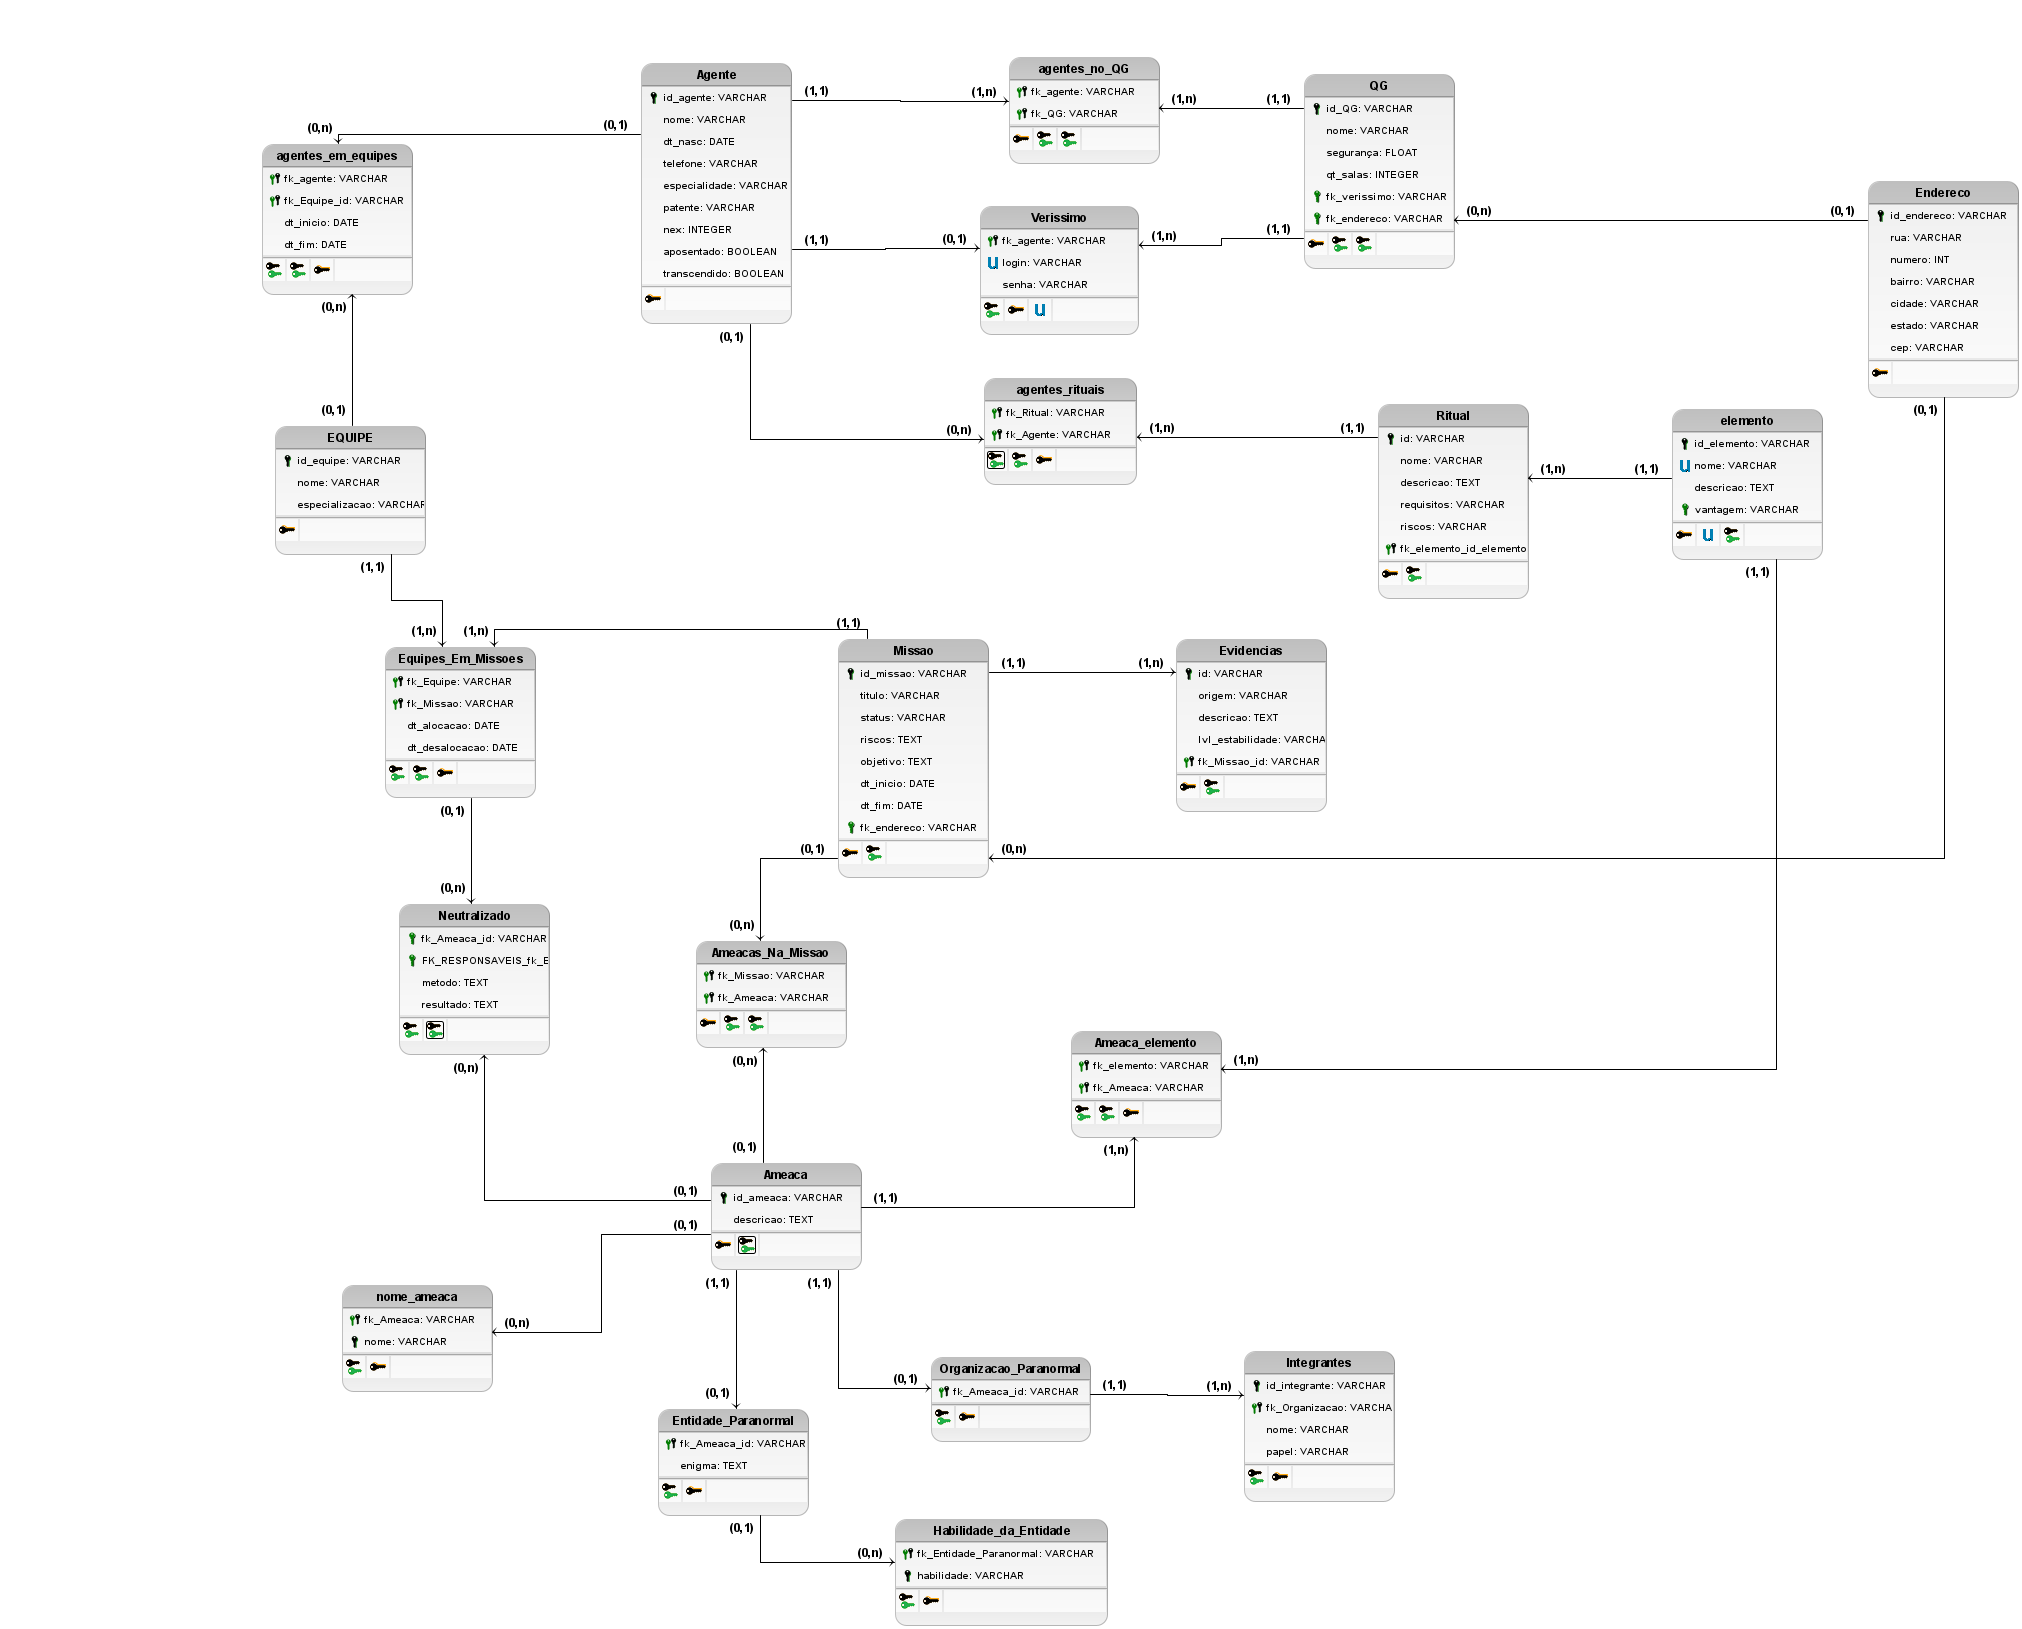
\includegraphics[width=1\textwidth]{Logico.png}
    \label{fig:logico}
\end{figure}
Modelo lógico feito pelos integrantes do grupo, baseado no modelo conceitual. Utilizado para a visualização e definição das tabelas, juntamente com as definições das chaves primárias, visualização das chaves secundárias e ajustes de relacionamentos.

\chapter{4. Requisitos}
\section{4.1 Requisitos de BD}
\begin{itemize}
    \item \textbf{Ter no mínimo 8 entidades: }
    \begin{itemize}
        \item 10 Entidades - Agente, Verissimo, QG, Elemento, Ritual, Equipe, Missão, Evidência, Ameaça, Integrantes
    \end{itemize}

    \item \textbf{Conceitos Obrigatótios: }
    \begin{itemize}
        \item Atributo Composto
            \begin{itemize}
                \item Localização - É um atributo composto - que está presente em QG e em missão -, que foi dividido em rua, nûmero, bairro, cidade e cep.
                Como ele está presente em mais de uma tabela foi criado uma tabela só de endereços para a melhor utilização no banco de dados.

            \begin{figure}[H]
                \centering
                    \begin{minipage}[b]{0.45\linewidth}
                        \centering
                        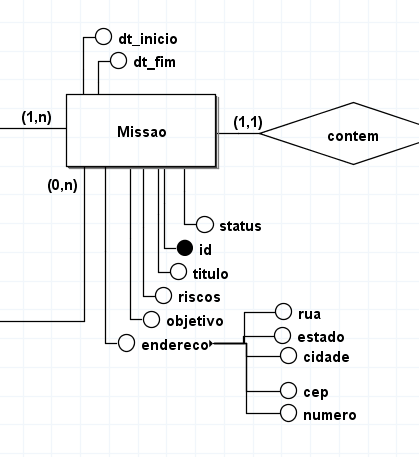
\includegraphics[width=\linewidth]{composto-missão.png}
                        \caption{Atributo Composto em Missão}
                        \label{fig:composto-missão}
                    \end{minipage}
                \hfill
                    \begin{minipage}[b]{0.45\linewidth}
                        \centering
                        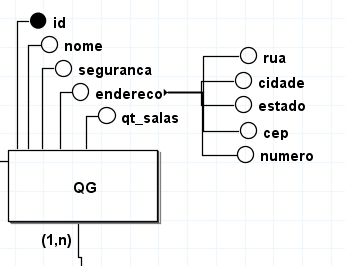
\includegraphics[width=\linewidth]{composto-qg.png}
                        \caption{Atributo Composto em QG}
                        \label{fig:herence-threats}
                    \end{minipage}
                \end{figure}
            \end{itemize}
            
        \item Atributo Multivalorado
            \begin{itemize}
                \item Nome de ameaças - As ameças podem ter mais de um nome, então foi criado uma tabela só para os nomes, como não ficou claro se era um valor máximo de nomes diferentes.
            \begin{figure}[H]
                \centering
                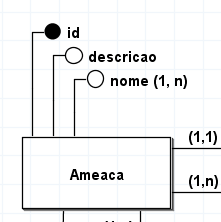
\includegraphics[width=0.5\linewidth]{multivalorado-nomes.png}
                \caption{Multivalorado}
                \label{fig:enter-label}
            \end{figure}
            \end{itemize}

            
        \item Cardinalidade Diversas
            \begin{itemize}
                \item Agente-Equipe = (1,N) (1,N)
                \item Verissimo-QG = (1,1) (1,N)
                \item Elemento-Elemento = (0,N) (0,N)
                \item Ritual-Transcendido = (0,N) (1,N)
            \end{itemize}
        \item Atributo de Relacionamento
            \begin{itemize}
                \item Temos tanto a data de alocação e data de desalocação no relacionamento entre equipe e missão.
                \item Temos o data de entrada e data de saída de membros em uma equipe.

                \begin{figure}[H]
                    \centering
                    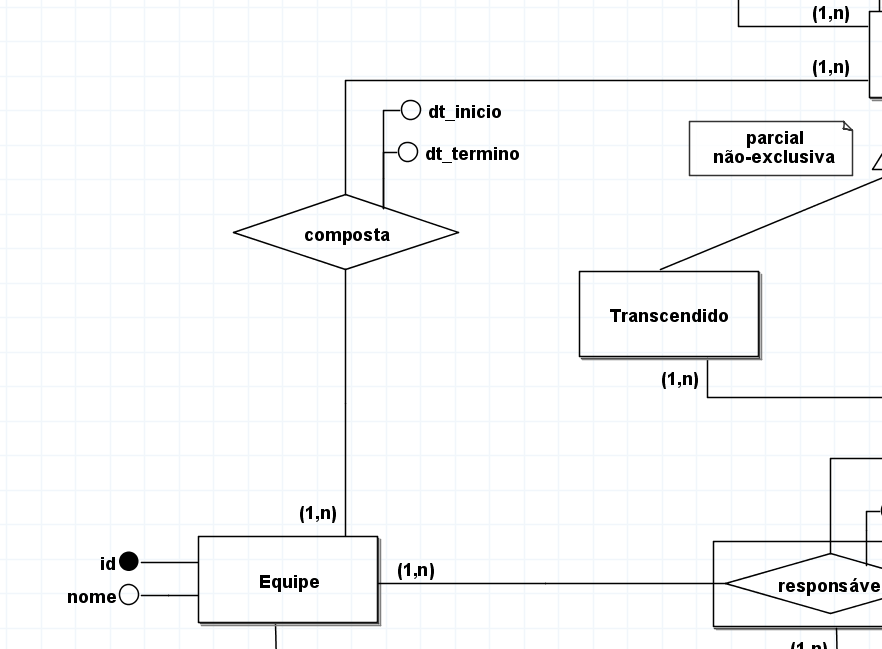
\includegraphics[width=0.5\linewidth]{relação-com-atributo.png}
                    \caption{Relção com atributo de Agente - Compoe - Equipe}
                    \label{fig:enter-label}
                \end{figure}
            \end{itemize}
        \item Auto-relacionamento
            \begin{itemize}
                \item Vantagem é um atributo do auto relacionamento do elememnto com ele mesmo
                \begin{figure}[H]
                    \centering
                    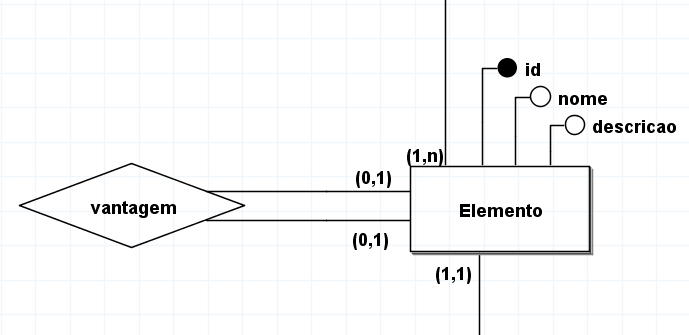
\includegraphics[width=0.5\linewidth]{auto-relacionamento.png}
                    \caption{Auto-Relacionamento}
                    \label{fig:enter-label}
                \end{figure}
            \end{itemize}

            
        \item Agregação ou Ternário
            \begin{itemize}
                \item O relacionamento Responsável e Neutralizado é isso, temos Equipe -> Responsável <- Missão. E apartir de responsável -> neutralizado <- ameaça
                \begin{figure}[H]
                    \centering
                    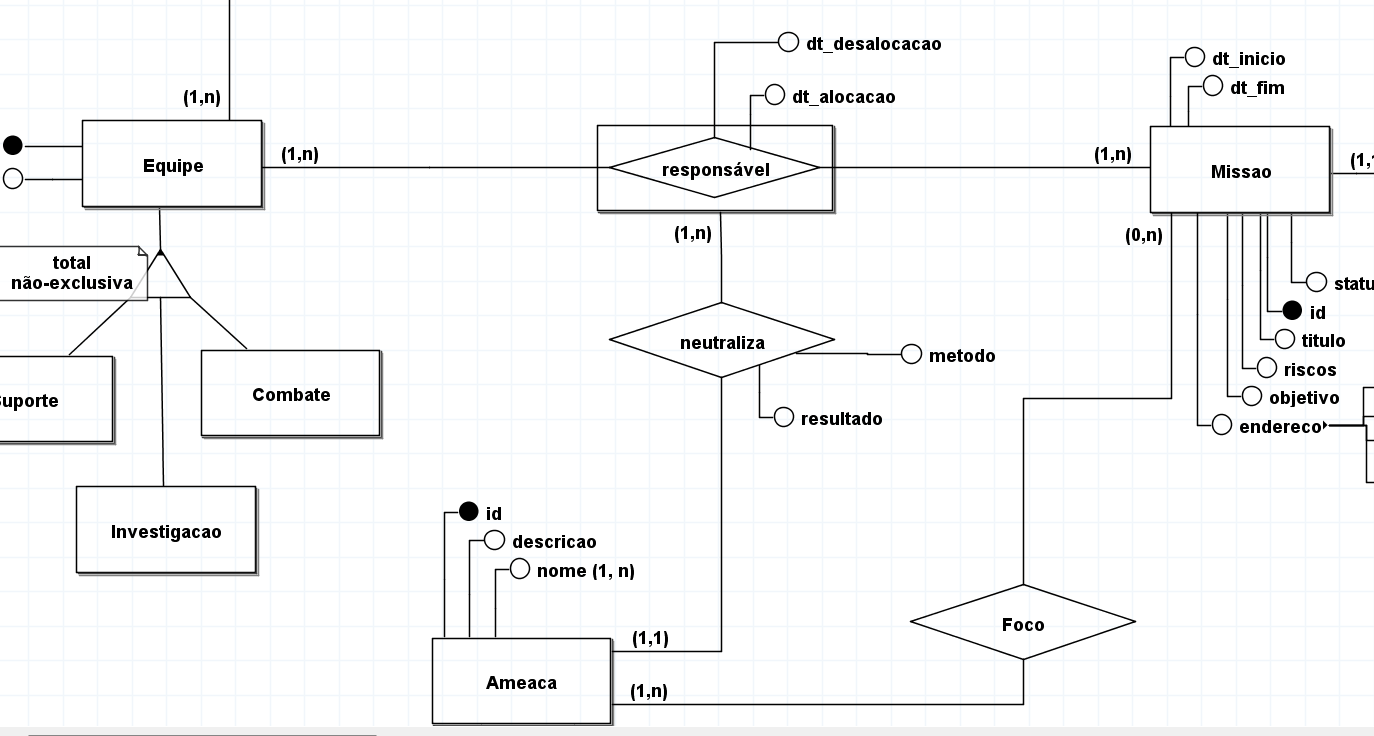
\includegraphics[width=0.5\linewidth]{relação_agregação.png}
                    \caption{Relação de agregação}
                    \label{fig:enter-label}
                \end{figure}
            \end{itemize}
            
        \item Entidade Fraca
            \begin{itemize}
                \item Os Integrantes de uma Ogranização Paranormal São uma entidade fraca. Eles só podem existir se tiver uma organização correspondente.
                \begin{figure}[H]
                    \centering
                    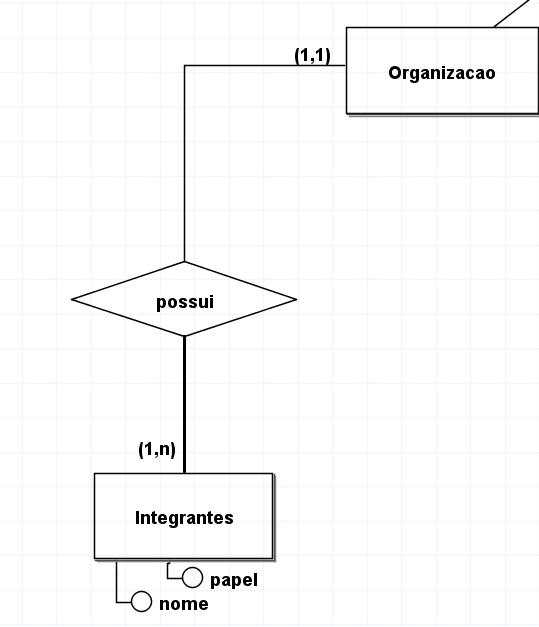
\includegraphics[width=0.5\linewidth]{entidade_fraca_intg.png}
                    \caption{Entidade fraca em integrande de organização}
                    \label{fig:enter-label}
                \end{figure}
            \end{itemize}
            
        \item Herança
        \begin{itemize}
            \item Agente tem como herança o verissimo e o transcendido, Equipe tem como herança suporte, combate e investigação e Ameaça tem como herança Entidade Paranormal e Ogranização Parnaormal
            \begin{figure}[H]
                \centering
                \begin{minipage}[b]{0.45\linewidth}
                \centering
                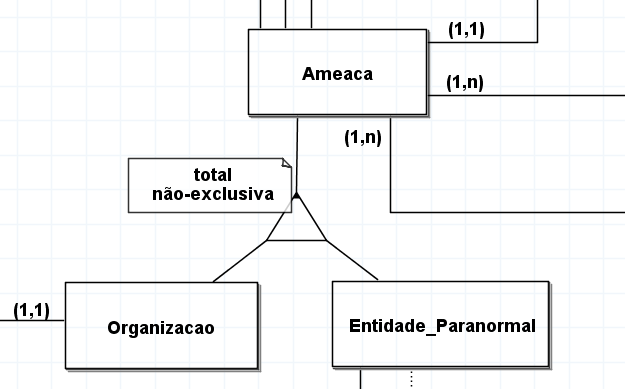
\includegraphics[width=\linewidth]{heranca_ameaca.png}
                \caption{Herança das Ameaças}
                \label{fig:herança-ameaças}
            \end{minipage}
            \hfill
                \begin{minipage}[b]{0.45\linewidth}
                \centering
                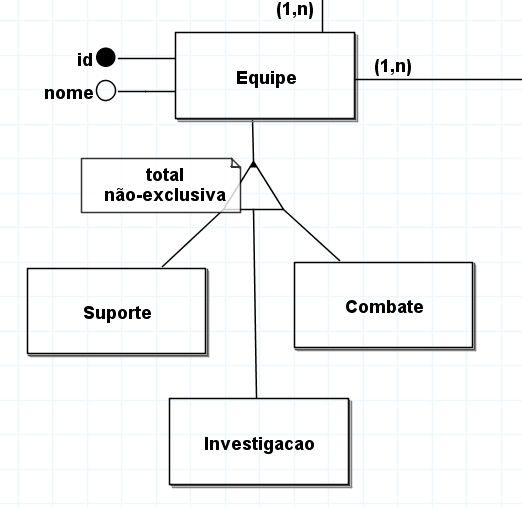
\includegraphics[width=\linewidth]{heranca_equipe.png}
                \caption{Herança das Ameaças}
                \label{fig:herence-threats}
            \end{minipage}
            \end{figure}
        \end{itemize}

        \item Extra
            \begin{itemize}
                \item Conceitos utilizados como default, not null e check in
                \begin{figure}[H]
                    \centering
                    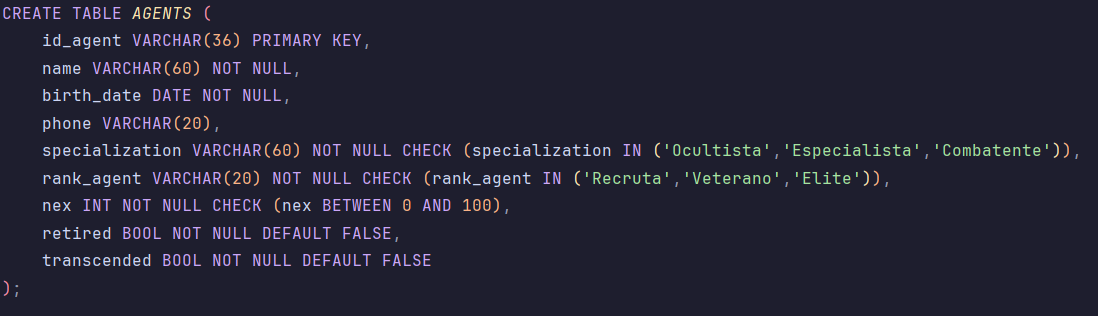
\includegraphics[width=1\linewidth]{agents_table.png}
                    \caption{Tabela de agentes com uso de default, check in e not null}
                    \label{fig:enter-label}
                \end{figure}
            \end{itemize}
    \end{itemize}
\end{itemize}
\section{4.2 Requisitos de Interface}

\subsection{4.2.1 Interface de CRUD}
    \begin{itemize}
            \item Adicionar dados
        \begin{description}
            \item Possibilita que o usuário adicione os dados e crie um novo agente a partir deles.
        \end{description}
    
        \begin{figure}[H]
            \centering
            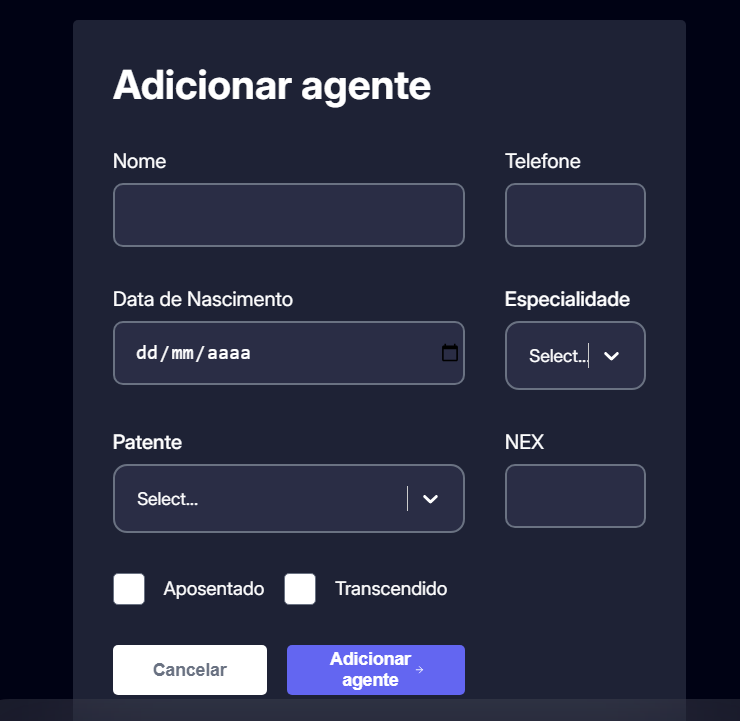
\includegraphics[width=0.5\linewidth]{agentes_create.png}
            \caption{Criar novo agente }
            \label{fig:enter-label}
        \end{figure}
        
        \item Vizualização dos dados
        \begin{description}
            \item Permite que o usuário possa vizualizar os dados de forma dinâmica e em tabela.
        \end{description}
        
        \begin{figure}[H]
            \centering
            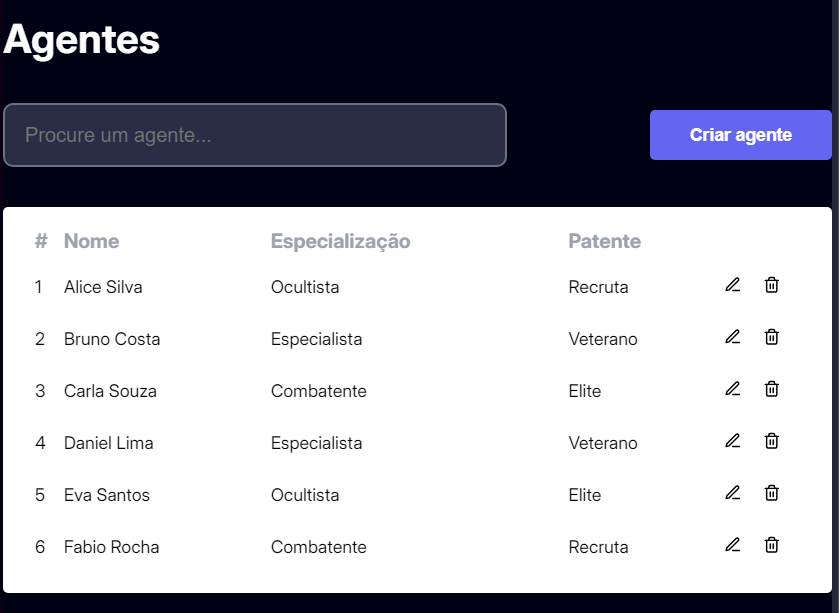
\includegraphics[width=0.5\linewidth]{agentes_read.png}
            \caption{Vizualização de agente}
            \label{fig:enter-label}
        \end{figure}

        \item Alterar dados
        \begin{description}
            \item Possibilita que o usuário altere os dados caso estejam desatualizados.
        \end{description}
        \begin{figure}[H]
            \centering
            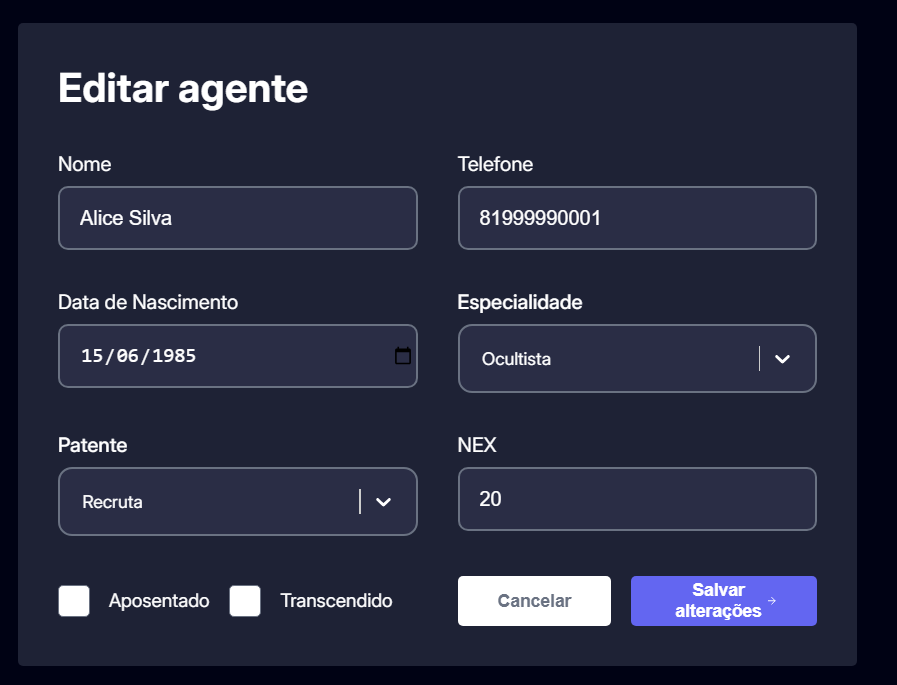
\includegraphics[width=0.5\linewidth]{agentes_update.png}
            \caption{Atualizar agente já existente}
            \label{fig:enter-label}
        \end{figure}

        \item Remover dados
        \begin{description}
            \item Possibilita o usuário a remover agentes.
        \end{description}
        \begin{figure}[H]
            \centering
            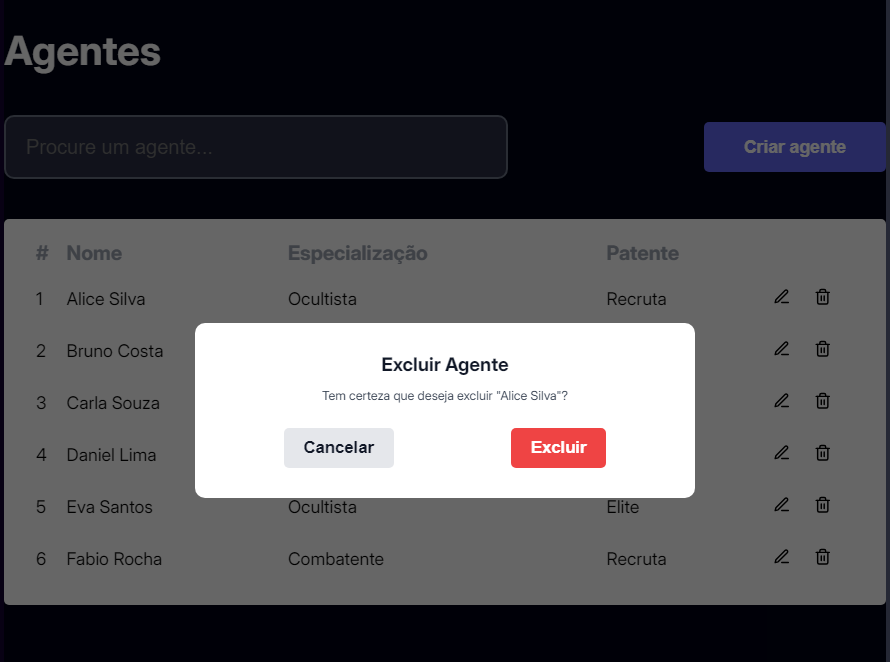
\includegraphics[width=0.5\linewidth]{agentes_remove.png}
            \caption{Remover agente já existente}
            \label{fig:enter-label}
        \end{figure}
    \end{itemize}

\subsection{4.2.2 Interface Funcional com Dashboard}
    \begin{itemize}
            \item Dashboards de dados de interesse para o usuário 
        \begin{description}
            \item Permite que o usuário (agente) possa visualizar os dados de interesse de uma maneira mais simples ao realizar o login na plataforma. Os dashboards disponíveis são "Agentes ativos", "Missões em andamento", "Missões Concluidas" e "Tempo médio".
        \end{description}
        
        \begin{figure}[H]
            \centering
            
\includegraphics[width=1\linewidth]{dashboard_dados_usuario.png}
            \caption{Dashboards do agente}
            \label{fig:enter-label}
        \end{figure}
        
            \item Dashboard das ocorrências de ameaças por elemento 
        \begin{description}
            \item Esse dashboard mostra gráficos do total de ocorrências de ameaças por elemento, filtrado for localidade. Útil para entender quais elementos são mais prováveis de aparecer em uma certa região.
        \end{description}
    
        \begin{figure}[H]
            \centering
            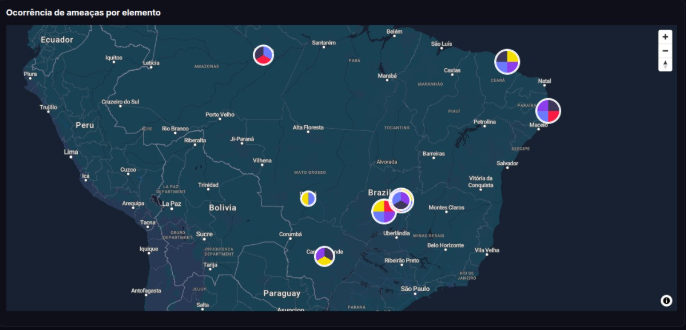
\includegraphics[width=1\linewidth]{dashboard_ameacas_por_elemento.png}
            \caption{Ocorrências de ameaças por elemento}
            \label{fig:enter-label}
        \end{figure}
        
        \item Dashboards de indicadores operacionais gerais
    \begin{description}
        \item Essa seção de dashboards apresentam indicadores agregados de desempenho e distribuição das operações da organização. É especialmente útil para coordenadores e administradores que desejam ter uma visão panorâmica dos dados operacionais. São exibidas informações como ranking de agentes com mais missões bem-sucedidas, média de NEX por QG, distribuição das equipes por especialização, status das missões (abertas ou concluídas) e quantidade de agentes por especialização.
    \end{description}
    
        \begin{figure}[H]
            \centering
            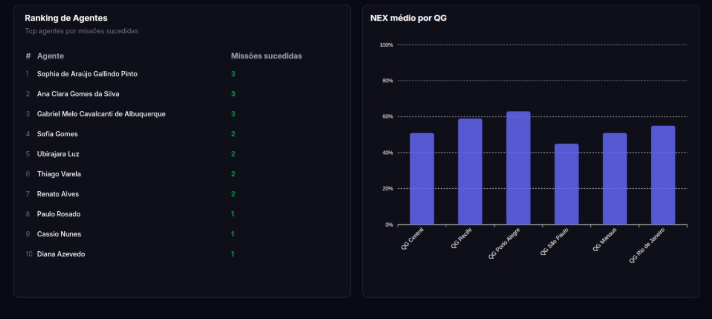
\includegraphics[width=1\linewidth]{dashboard_indicadores_op_1.png}
            \caption{Indicadores operacionais – Parte 1}
            \label{fig:dashboard-indicadores-1}
        \end{figure}

        \begin{figure}[H]
            \centering
            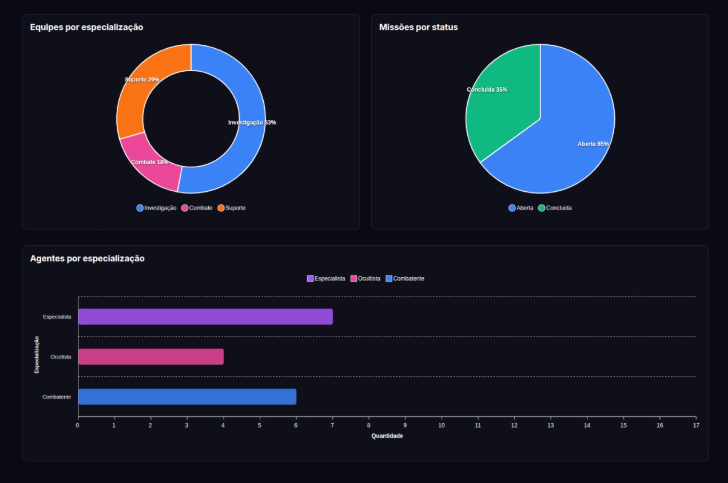
\includegraphics[width=1\linewidth]{dashboard_indicadores_op_2.png}
            \caption{Indicadores operacionais – Parte 2}
            \label{fig:dashboard-indicadores-2}
        \end{figure}
    \end{itemize}

\chapter{5. Scripts}
\section{5.1 Script de Criação das tabelas}
Esse script engloba todas as criações de tabelas realizadas no banco de dados.
\begin{lstlisting}[language=SQL, caption=ordemdb.sql]
create database IF NOT EXISTS ordemdb;
use ordemdb;
CREATE TABLE AGENTS (
    id_agent VARCHAR(36) PRIMARY KEY,
    name VARCHAR(60) NOT NULL,
    birth_date DATE NOT NULL,
    phone VARCHAR(20),
    specialization VARCHAR(60) NOT NULL CHECK (specialization IN ('Ocultista','Especialista','Combatente')),
    rank_agent VARCHAR(20) NOT NULL CHECK (rank_agent IN ('Recruta','Veterano','Elite')),
    nex INT NOT NULL CHECK (nex BETWEEN 0 AND 100),
    retired BOOL NOT NULL DEFAULT FALSE,
    transcended BOOL NOT NULL DEFAULT FALSE
);

CREATE TABLE VERISSIMO (
    id_verissimo VARCHAR(36) PRIMARY KEY,
    login VARCHAR(20) UNIQUE NOT NULL,
    password_ver VARCHAR(50) NOT NULL,
    FOREIGN KEY (id_verissimo) REFERENCES AGENTS(id_agent) ON DELETE CASCADE
);

CREATE TABLE ADDRESS (
    id_address VARCHAR(36) PRIMARY KEY,
    street VARCHAR(100) NOT NULL,
    number INT,
    neighborhood VARCHAR(60),
    city VARCHAR(60) NOT NULL,
    state CHAR(2) NOT NULL,
    postal_code CHAR(9)
);

CREATE TABLE HQ (
    id_hq VARCHAR(36) PRIMARY KEY,
    name VARCHAR(60) NOT NULL,
    security_level FLOAT NOT NULL DEFAULT 1.0 CHECK (security_level BETWEEN 0.0 AND 10.0),
    room_count INT NULL DEFAULT 1 CHECK (room_count > 0),
    id_address VARCHAR(36) NOT NULL,
    id_verissimo VARCHAR(36) NOT NULL,
    FOREIGN KEY (id_address) REFERENCES ADDRESS(id_address) ON DELETE CASCADE,
    FOREIGN KEY (id_verissimo) REFERENCES VERISSIMO(id_verissimo) ON DELETE CASCADE
);

CREATE TABLE AGENTS_IN_HQ (
    id_hq VARCHAR(36) NOT NULL,
    id_agent VARCHAR(36) NOT NULL,
    FOREIGN KEY (id_hq) REFERENCES HQ(id_hq) ON DELETE CASCADE,
    FOREIGN KEY (id_agent) REFERENCES AGENTS(id_agent) ON DELETE CASCADE,
    PRIMARY KEY (id_hq, id_agent)
);

CREATE TABLE TEAM (
    id_team VARCHAR(36) PRIMARY KEY,
    name VARCHAR(60) NOT NULL,
    specialization VARCHAR(60) NOT NULL CHECK (specialization IN ('Investigação','Combate','Suporte'))
);

CREATE TABLE AGENTS_IN_TEAM (
    id_team VARCHAR(36) NOT NULL,
    id_agent VARCHAR(36) NOT NULL,
    start_date DATETIME NOT NULL DEFAULT CURRENT_TIMESTAMP,
    end_date DATE,
    FOREIGN KEY (id_team) REFERENCES TEAM(id_team) ON DELETE CASCADE,
    FOREIGN KEY (id_agent) REFERENCES AGENTS(id_agent) ON DELETE CASCADE,
    PRIMARY KEY (id_agent, id_team)
);

CREATE TABLE ELEMENTS (
    id_element VARCHAR(36) PRIMARY KEY,
    name VARCHAR(15) NOT NULL UNIQUE,
    description TEXT NOT NULL,
    id_advantage VARCHAR(36),
    FOREIGN KEY (id_advantage) REFERENCES ELEMENTS(id_element) ON DELETE CASCADE
);

CREATE TABLE RITUALS (
    id_ritual VARCHAR(36) PRIMARY KEY,
    name VARCHAR(60) NOT NULL,
    description TEXT,
    requirements VARCHAR(100) NOT NULL,
    risks VARCHAR(100),
    id_element VARCHAR(36) NOT NULL,
    FOREIGN KEY (id_element) REFERENCES ELEMENTS(id_element) ON DELETE CASCADE
);

CREATE TABLE AGENT_RITUALS (
    id_agent VARCHAR(36) NOT NULL,
    id_ritual VARCHAR(36) NOT NULL,
    FOREIGN KEY (id_agent) REFERENCES AGENTS(id_agent) ON DELETE CASCADE,
    FOREIGN KEY (id_ritual) REFERENCES RITUALS(id_ritual) ON DELETE CASCADE,
    PRIMARY KEY (id_agent, id_ritual)
);

CREATE TABLE MISSION (
    id_mission VARCHAR(36) PRIMARY KEY,
    title VARCHAR(100) NOT NULL,
    status VARCHAR(20) NOT NULL CHECK (status IN ('Arquivada','Concluida','Aberta')) DEFAULT 'Aberta',
    risks TEXT NOT NULL,
    objective TEXT NOT NULL,
    start_date DATETIME NOT NULL DEFAULT CURRENT_TIMESTAMP,
    end_date DATE,
    id_address VARCHAR(36),
    id_hq VARCHAR(36),
    FOREIGN KEY (id_address) REFERENCES ADDRESS(id_address) ON DELETE CASCADE,
    FOREIGN KEY (id_hq) REFERENCES HQ(id_hq) ON DELETE CASCADE
);

CREATE TABLE MISSION_ASSIGNMENT (
    id_team VARCHAR(36) NOT NULL,
    id_mission VARCHAR(36) NOT NULL,
    allocation_date DATETIME NOT NULL DEFAULT CURRENT_TIMESTAMP,
    deallocation_date DATE,
    FOREIGN KEY (id_team) REFERENCES TEAM(id_team) ON DELETE CASCADE,
    FOREIGN KEY (id_mission) REFERENCES MISSION(id_mission) ON DELETE CASCADE,
    PRIMARY KEY (id_team, id_mission)
);

CREATE TABLE EVIDENCE (
    id_evidence VARCHAR(36) PRIMARY KEY,
    origin VARCHAR(100) NOT NULL,
    description TEXT NOT NULL,
    stability_level VARCHAR(30) NOT NULL CHECK (stability_level IN ('Estavel', 'Volatil', 'Perigoso', 'Contido')),
    id_mission VARCHAR(36) NOT NULL,
    FOREIGN KEY (id_mission) REFERENCES MISSION(id_mission) ON DELETE CASCADE
);

CREATE TABLE THREATS (
    id_threat VARCHAR(36) PRIMARY KEY,
    description TEXT NOT NULL
);

CREATE TABLE THREATS_NAMES (
    id_threat VARCHAR(36) NOT NULL,
    name VARCHAR(60) NOT NULL,
    FOREIGN KEY (id_threat) REFERENCES THREATS(id_threat) ON DELETE CASCADE,
    PRIMARY KEY (id_threat, name)
);

CREATE TABLE THREAT_MISSION (
    id_threat VARCHAR(36) NOT NULL,
    id_mission VARCHAR(36) NOT NULL,
    FOREIGN KEY (id_threat) REFERENCES THREATS(id_threat) ON DELETE CASCADE,
    FOREIGN KEY (id_mission) REFERENCES MISSION(id_mission) ON DELETE CASCADE,
    PRIMARY KEY (id_threat, id_mission)
);

CREATE TABLE THREAT_NEUTRALIZATION (
    id_team VARCHAR(36) NOT NULL,
    id_mission VARCHAR(36) NOT NULL,
    id_threat VARCHAR(36) NOT NULL,
    method TEXT NOT NULL,
    result TEXT NOT NULL,
    FOREIGN KEY (id_team, id_mission) REFERENCES MISSION_ASSIGNMENT(id_team, id_mission) ON DELETE CASCADE,
    FOREIGN KEY (id_threat) REFERENCES THREATS(id_threat) ON DELETE CASCADE,
    PRIMARY KEY (id_team, id_mission, id_threat)
);

CREATE TABLE THREAT_ELEMENTS (
    id_element VARCHAR(36) NOT NULL,
    id_threat VARCHAR(36) NOT NULL,
    FOREIGN KEY (id_element) REFERENCES ELEMENTS(id_element) ON DELETE CASCADE,
    FOREIGN KEY (id_threat) REFERENCES THREATS(id_threat) ON DELETE CASCADE,
    PRIMARY KEY (id_element, id_threat)
);

CREATE TABLE PARANORMAL_ENTITY (
    id_entity VARCHAR(36) PRIMARY KEY,
    enigma TEXT,
    FOREIGN KEY (id_entity) REFERENCES THREATS(id_threat) ON DELETE CASCADE
);

CREATE TABLE ENTITY_ABILITY (
    id_entity VARCHAR(36) NOT NULL,
    ability VARCHAR(255) NOT NULL,
    FOREIGN KEY (id_entity) REFERENCES PARANORMAL_ENTITY(id_entity) ON DELETE CASCADE,
    PRIMARY KEY (id_entity, ability)
);

CREATE TABLE PARANORMAL_ORGANIZATION (
    id_organization VARCHAR(36) PRIMARY KEY,
    FOREIGN KEY (id_organization) REFERENCES THREATS(id_threat) ON DELETE CASCADE
);

CREATE TABLE MEMBERS (
     id_member VARCHAR(36) PRIMARY KEY,
     id_organization VARCHAR(36) NOT NULL,
     name VARCHAR(60) NOT NULL,
     role VARCHAR(30) CHECK (role IN ('Lider', 'Pesquisador', 'Ocultista', 'Simpatizante')),
     FOREIGN KEY (id_organization) REFERENCES PARANORMAL_ORGANIZATION(id_organization) ON DELETE CASCADE
);

DELIMITER $$

CREATE FUNCTION VERIFY_NEX(nex INT)
    RETURNS BOOLEAN
    DETERMINISTIC
BEGIN
    IF nex >= 50 THEN
        RETURN TRUE;
    ELSE
        RETURN FALSE;

\end{lstlisting}
\section{5.2 Script de Inserção e Povoamento}
Script usado para povoar os campos das tabelas anteriormente criadas

\begin{lstlisting}[language=SQL, caption=population.sql]
-- Gerando UUIDs para todas as entidades
-- ===================================================================
-- Agentes
SET
@ag1=UUID(), @ag2=UUID(), @ag3=UUID(), @ag4=UUID(), @ag5=UUID(), @ag6=UUID(), @ag7=UUID(), @ag8=UUID(), @ag9=UUID(), @ag10=UUID(),
@ag11=UUID(), @ag12=UUID(), @ag13=UUID(), @ag14=UUID(), @ag15=UUID(), @ag16=UUID(), @ag17=UUID(), @ag18=UUID(), @ag19=UUID(), @ag20=UUID(),
@ag21=UUID(), @ag22=UUID(), @ag23=UUID(), @ag24=UUID(), @ag25=UUID(), @ag26=UUID(), @ag27=UUID(), @ag28=UUID(), @ag29=UUID(), @ag30=UUID(),
@ag31=UUID(), @ag32=UUID(), @ag33=UUID(), @ag34=UUID(), @ag35=UUID(), @ag36=UUID(), @ag37=UUID(), @ag38=UUID(), @ag39=UUID(), @ag40=UUID(),
@ag41=UUID(), @ag42=UUID(), @ag43=UUID(), @ag44=UUID(), @ag45=UUID(), @ag46=UUID(), @ag47=UUID(), @ag48=UUID(), @ag49=UUID(), @ag50=UUID(),
@ag51=UUID(), @ag52=UUID(), @ag53=UUID(), @ag54=UUID(), @ag55=UUID(), @ag56=UUID(), @ag57=UUID(), @ag58=UUID(), @ag59=UUID(), @ag60=UUID(),
@ag61=UUID(), @ag62=UUID(), @ag63=UUID(), @ag64=UUID(), @ag65=UUID(), @ag66=UUID(), @ag67=UUID(), @ag68=UUID(), @ag69=UUID(), @ag70=UUID(),
@ag71=UUID(), @ag72=UUID(), @ag73=UUID(), @ag74=UUID(), @ag75=UUID(), @ag76=UUID(), @ag77=UUID(), @ag78=UUID(), @ag79=UUID(), @ag80=UUID(),
@ag81=UUID(), @ag82=UUID(), @ag83=UUID(), @ag84=UUID(), @ag85=UUID(), @ag86=UUID(), @ag87=UUID(), @ag88=UUID(), @ag89=UUID(), @ag90=UUID(),
@ag91=UUID(), @ag92=UUID(), @ag93=UUID(), @ag94=UUID(), @ag95=UUID(), @ag96=UUID(), @ag97=UUID(), @ag98=UUID(), @ag99=UUID(), @ag100=UUID();



-- ===================================================================
-- Verissimos
SET
@ver1 = @ag2, @ver2=@ag25, @ver3=@ag49, @ver4=@ag57, @ver5=@ag75, @ver6=@ag94;

-- ===================================================================
-- Endereços
SET
@addr1  = UUID(), @addr2  = UUID(), @addr3  = UUID(), @addr4  = UUID(), @addr5  = UUID(),
@addr6  = UUID(), @addr7  = UUID(), @addr8  = UUID(), @addr9  = UUID(), @addr10 = UUID(),
@addr11 = UUID(), @addr12 = UUID(), @addr13 = UUID(), @addr14 = UUID(), @addr15 = UUID(),
@addr16 = UUID(), @addr17 = UUID(), @addr18 = UUID(), @addr19 = UUID(), @addr20 = UUID(),
@addr21 = UUID(), @addr22 = UUID(), @addr23 = UUID(), @addr24 = UUID(), @addr25 = UUID(),
@addr26 = UUID(), @addr27 = UUID(), @addr28 = UUID(), @addr29 = UUID(), @addr30 = UUID(),
@addr31 = UUID(), @addr32 = UUID(), @addr33 = UUID(), @addr34 = UUID(), @addr35 = UUID(),
@addr36 = UUID(), @addr37 = UUID(), @addr38 = UUID(), @addr39 = UUID(), @addr40 = UUID(),
@addr41 = UUID(), @addr42 = UUID(), @addr43 = UUID(), @addr44 = UUID(), @addr45 = UUID(),
@addr46 = UUID(), @addr47 = UUID(), @addr48 = UUID(), @addr49 = UUID(), @addr50 = UUID(),
@addr51 = UUID(), @addr52 = UUID(), @addr53 = UUID(), @addr54 = UUID(), @addr55 = UUID(),
@addr56 = UUID(), @addr57 = UUID(), @addr58 = UUID(), @addr59 = UUID(), @addr60 = UUID(),
@addr61 = UUID(), @addr62 = UUID(), @addr63 = UUID(), @addr64 = UUID(), @addr65 = UUID(),
@addr66 = UUID(), @addr67 = UUID(), @addr68 = UUID(), @addr69 = UUID(), @addr70 = UUID(),
@addr71 = UUID(), @addr72 = UUID(), @addr73 = UUID(), @addr74 = UUID(), @addr75 = UUID(),
@addr76 = UUID(), @addr77 = UUID(), @addr78 = UUID(), @addr79 = UUID(), @addr80 = UUID(),
@addr81 = UUID(), @addr82 = UUID(), @addr83 = UUID(), @addr84 = UUID(), @addr85 = UUID(),
@addr86 = UUID(), @addr87 = UUID(), @addr88 = UUID(), @addr89 = UUID(), @addr90 = UUID(),
@addr91 = UUID(), @addr92 = UUID(), @addr93 = UUID(), @addr94 = UUID(), @addr95 = UUID(),
@addr96 = UUID(), @addr97 = UUID(), @addr98 = UUID(), @addr99 = UUID(), @addr100 = UUID();


-- ===================================================================
-- QGs
SET @hq1= UUID(), @hq2=UUID(),   @hq3=UUID(), @hq4=UUID(), @hq5=UUID(), @hq6=UUID();

-- ===================================================================
-- Equipes
SET
@team1  = UUID(),  @team2  = UUID(),  @team3  = UUID(),  @team4  = UUID(),
@team5  = UUID(),  @team6  = UUID(),  @team7  = UUID(),  @team8  = UUID(),
@team9  = UUID(),  @team10 = UUID(),  @team11 = UUID(),  @team12 = UUID(),
@team13  = UUID(),  @team14 = UUID(),  @team15 = UUID(),  @team16 = UUID(),
@team17  = UUID(),  @team18 = UUID(),  @team19 = UUID(),  @team20 = UUID(),
@team21  = UUID(),  @team22 = UUID(),  @team23 = UUID(),  @team24 = UUID(),
@team25  = UUID(),  @team26 = UUID(),  @team27 = UUID(),  @team28 = UUID();

-- ===================================================================
-- Elementos
SET @elMedo   = UUID();
SET @elMorte  = UUID();
SET @elSangue = UUID();
SET @elConhe  = UUID();
SET @elEnergia= UUID();

-- ===================================================================
-- Rituais
SET
@rit1=UUID(),  @rit2=UUID(),  @rit3=UUID(),  @rit4=UUID(),  @rit5=UUID(),
@rit6=UUID(),  @rit7=UUID(),  @rit8=UUID(),  @rit9=UUID(),  @rit10=UUID(),
@rit11=UUID(), @rit12=UUID(), @rit13=UUID(), @rit14=UUID(), @rit15=UUID();

-- ===================================================================
-- Missões
SET
@miss1   = UUID(), @miss2   = UUID(), @miss3   = UUID(), @miss4   = UUID(), @miss5   = UUID(),
@miss6   = UUID(), @miss7   = UUID(), @miss8   = UUID(), @miss9   = UUID(), @miss10  = UUID(),
@miss11  = UUID(), @miss12  = UUID(), @miss13  = UUID(), @miss14  = UUID(), @miss15  = UUID(),
@miss16  = UUID(), @miss17  = UUID(), @miss18  = UUID(), @miss19  = UUID(), @miss20  = UUID(),
@miss21  = UUID(), @miss22  = UUID(), @miss23  = UUID(), @miss24  = UUID(), @miss25  = UUID(),
@miss26  = UUID(), @miss27  = UUID(), @miss28  = UUID(), @miss29  = UUID(), @miss30  = UUID(),
@miss31  = UUID(), @miss32  = UUID(), @miss33  = UUID(), @miss34  = UUID(), @miss35  = UUID(),
@miss36  = UUID(), @miss37  = UUID(), @miss38  = UUID(), @miss39  = UUID(), @miss40  = UUID(),
@miss41  = UUID(), @miss42  = UUID(), @miss43  = UUID(), @miss44  = UUID(), @miss45  = UUID(),
@miss46  = UUID(), @miss47  = UUID(), @miss48  = UUID(), @miss49  = UUID(), @miss50  = UUID(),
@miss51  = UUID(), @miss52  = UUID(), @miss53  = UUID(), @miss54  = UUID(), @miss55  = UUID(),
@miss56  = UUID(), @miss57  = UUID(), @miss58  = UUID(), @miss59  = UUID(), @miss60  = UUID(),
@miss61  = UUID(), @miss62  = UUID(), @miss63  = UUID(), @miss64  = UUID(), @miss65  = UUID(),
@miss66  = UUID(), @miss67  = UUID(), @miss68  = UUID(), @miss69  = UUID(), @miss70  = UUID(),
@miss71  = UUID(), @miss72  = UUID(), @miss73  = UUID(), @miss74  = UUID(), @miss75  = UUID(),
@miss76  = UUID(), @miss77  = UUID(), @miss78  = UUID(), @miss79  = UUID(), @miss80  = UUID(),
@miss81  = UUID(), @miss82  = UUID(), @miss83  = UUID(), @miss84  = UUID(), @miss85  = UUID(),
@miss86  = UUID(), @miss87  = UUID(), @miss88  = UUID(), @miss89  = UUID(), @miss90  = UUID(),
@miss91  = UUID(), @miss92  = UUID(), @miss93  = UUID(), @miss94  = UUID(), @miss95  = UUID(),
@miss96  = UUID(), @miss97  = UUID(), @miss98  = UUID(), @miss99  = UUID(), @miss100 = UUID(),
@miss101  = UUID(), @miss102  = UUID(), @miss103  = UUID(), @miss104  = UUID(), @miss105 = UUID(),
@miss106  = UUID(), @miss103  = UUID(), @miss104  = UUID(), @miss105  = UUID(), @miss106 = UUID(),
@miss107  = UUID(), @miss108  = UUID(), @miss109  = UUID(), @miss110  = UUID(), @miss111 = UUID(),
@miss111  = UUID(), @miss112  = UUID(), @miss113  = UUID(), @miss114  = UUID(), @miss115 = UUID(),
@miss116  = UUID(), @miss117  = UUID(), @miss118  = UUID(), @miss119  = UUID(), @miss120 = UUID();

-- ===================================================================
-- Evidencias
SET
@evid1 = UUID(),  @evid2 = UUID(),  @evid3 = UUID(),
@evid4 = UUID(),  @evid5 = UUID(),  @evid6 = UUID(),
@evid7 = UUID(),  @evid8 = UUID(),  @evid9 = UUID(),
@evid10 = UUID(), @evid11 = UUID(), @evid12 = UUID(),
@evid13 = UUID(), @evid14 = UUID(), @evid15 = UUID(),
@evid16 = UUID(), @evid17 = UUID(), @evid18 = UUID(),
@evid19 = UUID(), @evid20 = UUID(), @evid21 = UUID(),
@evid22 = UUID(), @evid23 = UUID(), @evid24 = UUID(),
@evid25 = UUID(), @evid26 = UUID(), @evid27 = UUID(),
@evid28 = UUID(), @evid29 = UUID(), @evid30 = UUID(),
@evid31 = UUID(), @evid32 = UUID(), @evid33 = UUID(),
@evid34 = UUID(), @evid35 = UUID(), @evid36 = UUID(),
@evid37 = UUID(), @evid38 = UUID(), @evid39 = UUID(),
@evid40 = UUID(), @evid41 = UUID(), @evid42 = UUID(),
@evid43 = UUID(), @evid44 = UUID(), @evid45 = UUID(),
@evid46 = UUID(), @evid47 = UUID(), @evid48 = UUID(),
@evid49 = UUID(), @evid50 = UUID(), @evid51 = UUID(),
@evid52 = UUID(), @evid53 = UUID(), @evid54 = UUID(),
@evid55 = UUID(), @evid56 = UUID(), @evid57 = UUID(),
@evid58 = UUID(), @evid59 = UUID(), @evid60 = UUID(),
@evid61 = UUID(), @evid62 = UUID(), @evid63 = UUID(),
@evid64 = UUID(), @evid65 = UUID(), @evid66 = UUID(),
@evid67 = UUID(), @evid68 = UUID(), @evid69 = UUID(),
@evid70 = UUID(), @evid71 = UUID(), @evid72 = UUID(),
@evid73 = UUID(), @evid74 = UUID();



-- ===================================================================
-- Ameaças
SET
@thr1 = UUID(),  @thr2 = UUID(),  @thr3 = UUID(),  @thr4 = UUID(),  @thr5 = UUID(),
@thr6 = UUID(),  @thr7 = UUID(),  @thr8 = UUID(),  @thr9 = UUID(),  @thr10 = UUID(),
@thr11 = UUID(), @thr12 = UUID(), @thr13 = UUID(), @thr14 = UUID(), @thr15 = UUID(),
@thr16 = UUID(), @thr17 = UUID(), @thr18 = UUID(), @thr19 = UUID(), @thr20 = UUID(),
@thr21 = UUID(), @thr22 = UUID(), @thr23 = UUID(), @thr24 = UUID(), @thr25 = UUID(),
@thr26 = UUID(), @thr27 = UUID(), @thr28 = UUID(), @thr29 = UUID(), @thr30 = UUID(),
@thr31 = UUID(), @thr32 = UUID(), @thr33 = UUID(), @thr34 = UUID(), @thr35 = UUID(),
@thr36 = UUID(), @thr37 = UUID(), @thr38 = UUID(), @thr39 = UUID(), @thr40 = UUID(),
@thr41 = UUID(), @thr42 = UUID(), @thr43 = UUID(), @thr44 = UUID(), @thr45 = UUID(),
@thr46 = UUID(), @thr47 = UUID();

-- ===================================================================
-- Membros-organizações
SET
@mem1=UUID(),  @mem2=UUID(),  @mem3=UUID(),  @mem4=UUID(),
@mem5=UUID(),  @mem6=UUID(),  @mem7=UUID(),  @mem8=UUID(),
@mem9=UUID(),  @mem10=UUID(), @mem11=UUID(), @mem12=UUID(),
@mem13=UUID(), @mem14=UUID(), @mem15=UUID(), @mem16=UUID(),
@mem17=UUID(), @mem18=UUID(), @mem19=UUID(), @mem20=UUID(),
@mem21=UUID(), @mem22=UUID(), @mem23=UUID(), @mem24=UUID(),
@mem25=UUID(), @mem26=UUID(), @mem27=UUID(), @mem28=UUID(),
@mem29=UUID(), @mem30=UUID(), @mem31=UUID(), @mem32=UUID(),
@mem33=UUID(), @mem34=UUID(), @mem35=UUID(), @mem36=UUID(),
@mem37=UUID(), @mem38=UUID(), @mem39=UUID(), @mem40=UUID(),
@mem41=UUID(), @mem42=UUID(), @mem43=UUID(), @mem44=UUID(),
@mem45=UUID(), @mem46=UUID(), @mem47=UUID(), @mem48=UUID(),
@mem49=UUID(), @mem50=UUID(), @mem51=UUID(), @mem52=UUID(),
@mem53=UUID(), @mem54=UUID(), @mem55=UUID(), @mem56=UUID(),
@mem57=UUID(), @mem58=UUID(), @mem59=UUID(), @mem60=UUID(),
@mem61=UUID(), @mem62=UUID(), @mem63=UUID(), @mem64=UUID();

-- ===================================================================
-- População de AGENTS OK
INSERT INTO AGENTS (id_agent, name, birth_date, phone, specialization, rank_agent, nex, retired, transcended) VALUES
-- QG1
(@ag1,  'Alice Silva',        '1985-06-15', '81999990001', 'Ocultista',   'Recruta',  20, FALSE, FALSE),
(@ag2,  'Bruno Costa',        '1978-02-20', '81999990002', 'Especialista','Veterano', 45, FALSE, FALSE), -- VER 1 
(@ag3,  'Carla Souza',        '1990-10-05', '81999990003', 'Combatente',  'Elite',    85, FALSE, TRUE),
(@ag4,  'Daniel Lima',        '1970-12-01', '81999990004', 'Especialista','Veterano', 60, FALSE, FALSE),
(@ag5,  'Eva Santos',         '1982-03-12', '82999990005', 'Ocultista',   'Elite',    95, FALSE, TRUE),
(@ag6,  'Fabio Rocha',        '1995-07-30', '87999990006', 'Combatente',  'Recruta',  10, FALSE, FALSE),
(@ag7,  'Gustavo Pires',      '1981-01-10', '11999990007', 'Especialista','Recruta',  25, FALSE, FALSE),
(@ag8,  'Helena Dias',        '1984-05-22', '11999990008', 'Ocultista',   'Veterano', 50, TRUE,  FALSE),
(@ag9,  'Igor Almeida',       '1979-11-11', '11999990009', 'Combatente',  'Elite',    90, FALSE, FALSE),
(@ag10, 'Juliana Freitas',    '1992-08-17', '11999990010', 'Combatente',  'Recruta',  15, FALSE, FALSE),
(@ag11, 'Karina Moura',       '1986-04-03', '11999990011', 'Ocultista',   'Veterano', 55, FALSE, FALSE),
(@ag12, 'Lucas Batista',      '1988-09-29', '11999990012', 'Especialista','Elite',    80, FALSE, FALSE),
(@ag13, 'Mariana Costa',      '1991-12-05', '21999990013', 'Combatente',  'Veterano', 65, FALSE, FALSE),
(@ag14, 'Nicolas Horn',       '1975-07-07', '21999990014', 'Especialista','Recruta',  18, FALSE, FALSE),
(@ag15, 'Olivia Reis',        '1983-02-14', '21999990015', 'Ocultista',   'Elite',    88, FALSE, TRUE),
(@ag16, 'Pedro Lima',         '1976-06-21', '21999990016', 'Combatente',  'Veterano', 58, FALSE, FALSE),
(@ag17, 'Quesia Tavares',     '1989-03-30', '11999990017', 'Especialista','Recruta',  22, FALSE, FALSE),
-- QG2
(@ag18, 'Renato Alves',       '1993-10-12', '11999990018', 'Especialista','Veterano', 47, FALSE, FALSE),
(@ag19, 'Sofia Gomes',        '1987-11-25', '11999990019', 'Ocultista',   'Elite',    92, FALSE, TRUE),
(@ag20, 'Thiago Varela',      '1990-01-18', '11999990020', 'Combatente',  'Recruta',  12, FALSE, FALSE),
(@ag21, 'Ubirajara Luz',      '1972-08-08', '81999990021', 'Especialista','Veterano', 60, FALSE, FALSE),
(@ag22, 'Gustavo Mourato',    '1979-03-03', '17967890123', 'Especialista','Veterano', 62, FALSE, FALSE),
(@ag23, 'Vinicius de Andrade','1986-11-11', '47978901234', 'Combatente',  'Elite',    96, TRUE,  FALSE),
(@ag24, 'Luan Hiroshi Kato',  '1991-02-02', '67989012345', 'Ocultista',   'Veterano', 61, FALSE, FALSE),
(@ag25, 'Gabriel Melo',       '1993-06-06', '87990123456', 'Especialista','Elite',    48, FALSE, FALSE), -- VER 2
(@ag26, 'Ana Clara Gomes',    '1984-09-09', '97901234567', 'Combatente',  'Veterano', 59, FALSE, FALSE),
(@ag27, 'Sophia Gallindo',    '1978-04-04', '17912345678', 'Ocultista',   'Elite',    67, FALSE, FALSE),
(@ag28, 'Paulo Rosado',       '1989-01-01', '37923456789', 'Especialista','Veterano', 64, FALSE, FALSE),
(@ag29, 'Cassio Nunes',       '1983-06-06', '81999990029', 'Especialista','Elite',    82, FALSE, TRUE),
(@ag30, 'Diana Azevedo',      '1989-09-09', '81999990030', 'Combatente',  'Veterano', 57, FALSE, FALSE),
(@ag31, 'Camila Andrade',     '1988-02-05', '31934567890', 'Combatente',  'Elite',    95, FALSE, FALSE),
(@ag32, 'Diego Ferreira',     '1979-11-17', '41945678901', 'Ocultista',   'Veterano', 60, FALSE, FALSE),
(@ag33, 'Eduarda Gomes',      '1992-06-30', '51956789012', 'Especialista','Recruta',  20, FALSE, FALSE),
(@ag34, 'Felipe Ramos',       '1983-01-22', '61967890123', 'Combatente',  'Veterano', 50, FALSE, TRUE),
-- QG3
(@ag35, 'Gabriela Melo',      '1995-08-14', '71978901234', 'Ocultista',   'Elite',    88, FALSE, FALSE),
(@ag36, 'Henrique Alves',     '1981-12-09', '81989012345', 'Especialista','Veterano', 65, FALSE, FALSE),
(@ag37, 'Isabela Pinto',      '1993-03-19', '91990123456', 'Combatente',  'Recruta',  25, FALSE, FALSE),
(@ag38, 'João Duarte',        '1977-07-27', '95901234567', 'Ocultista',   'Veterano', 55, FALSE, FALSE),
(@ag39, 'Karina Santos',      '1986-10-03', '47912345678', 'Especialista','Elite',    92, FALSE, FALSE),
(@ag40, 'Leonardo Vieira',    '1980-05-11', '67923456789', 'Combatente',  'Veterano', 58, FALSE, FALSE),
(@ag41, 'Mariana Lopes',      '1991-12-25', '27934567890', 'Ocultista',   'Recruta',  35, FALSE, FALSE),
(@ag42, 'Nicolas Rocha',      '1984-04-04', '37945678901', 'Especialista','Veterano', 63, FALSE, FALSE),
(@ag43, 'Olívia Castro',      '1996-09-18', '57956789012', 'Combatente',  'Elite',    99, TRUE, FALSE),
(@ag44, 'Pedro Martins',      '1978-02-28', '77967890123', 'Ocultista',   'Veterano', 68, FALSE, FALSE),
(@ag45, 'Quésia Lima',        '1989-11-11', '87978901234', 'Especialista','Recruta',  22, FALSE, FALSE),
(@ag46, 'Ricardo Moura',      '1982-06-06', '97989012345', 'Combatente',  'Veterano', 57, FALSE, FALSE),
(@ag47, 'Sofia Teixeira',     '1994-03-23', '17990123456', 'Ocultista',   'Elite',    94, FALSE, FALSE),
(@ag48, 'Tiago Sousa',        '1976-08-08', '27901234567', 'Especialista','Veterano', 66, FALSE, FALSE),
(@ag49, 'Úrsula Nunes',       '1987-01-15', '47912345678', 'Combatente',  'Elite',    49, FALSE, FALSE), -- VER 3
(@ag50, 'Vitor Braga',        '1990-05-05', '67923456789', 'Ocultista',   'Veterano', 71, FALSE, FALSE),
(@ag51, 'Wagner Melo',        '1983-10-10', '87934567890', 'Especialista','Elite',    89, FALSE, FALSE),
-- QG4
(@ag52, 'Ximena Farias',      '1992-12-12', '97945678901', 'Combatente',  'Veterano', 54, FALSE, FALSE),
(@ag53, 'Yara Costa',         '1985-07-07', '37956789012', 'Ocultista',   'Recruta',  33, FALSE, FALSE),
(@ag54, 'Valéria Rocha',      '1985-09-09', '81999990022', 'Combatente',  'Recruta',  14, FALSE, FALSE),
(@ag55, 'Wellington Paz',     '1982-03-03', '81999990023', 'Combatente',  'Elite',    85, FALSE, TRUE),
(@ag56, 'Ximena Duarte',      '1994-12-12', '81999990024', 'Ocultista',   'Veterano', 53, TRUE,  FALSE),
(@ag57, 'Yuri Santana',       '1988-07-07', '81999990025', 'Especialista','Elite',    50, FALSE, TRUE), -- VER 4
(@ag58, 'Zara Pinto',         '1992-10-10', '81999990026', 'Combatente',  'Elite',    89, FALSE, TRUE),
(@ag59, 'Alan Cardoso',       '1977-05-05', '81999990027', 'Combatente',  'Veterano', 63, FALSE, FALSE),  
(@ag60, 'Beatriz Silva',      '1991-02-02', '81999990028', 'Ocultista',   'Recruta',  17, FALSE, FALSE),
(@ag61, 'Eduarda Ramos',      '1988-04-12', '87999990061', 'Ocultista',   'Recruta',  10, FALSE, FALSE),
(@ag62, 'Felipe Andrade',     '1992-11-03', '87999990062', 'Combatente',  'Veterano', 35, FALSE, FALSE),
(@ag63, 'Gabriela Melo',      '1984-08-27', '87999990063', 'Especialista','Veterano', 50, FALSE, FALSE),
(@ag64, 'Henrique Duarte',    '1975-06-15', '82999990064', 'Ocultista',   'Elite',    95, FALSE, TRUE),
(@ag65, 'Isabela Rocha',      '1995-01-19', '82999990065', 'Combatente',  'Recruta',  15, FALSE, FALSE),
(@ag66, 'João Pedro Lima',    '1981-09-10', '82999990066', 'Especialista','Veterano', 40, FALSE, FALSE),
(@ag67, 'Karen Nunes',        '1986-03-24', '67999990067', 'Ocultista',   'Veterano', 55, FALSE, FALSE),
-- QG5
(@ag68, 'Lucas Fernandes',    '1990-07-06', '67999990068', 'Combatente',   'Elite',    88, FALSE, FALSE),
(@ag69, 'Marina Teixeira',    '1989-10-30', '67999990069', 'Especialista', 'Veterano', 38, FALSE, FALSE),
(@ag70, 'Nicolas Castro',     '1982-12-11', '77999990070', 'Ocultista',    'Veterano', 65, FALSE, FALSE),
(@ag71, 'Olívia Martins',     '1993-05-22', '67999990071', 'Combatente',   'Recruta',  12, FALSE, FALSE),
(@ag72, 'Paulo Henrique',     '1976-02-17', '67999990072', 'Especialista', 'Elite',    91, FALSE, TRUE),
(@ag73, 'Quésia Lopes',       '1987-11-08', '67999990073', 'Ocultista',    'Veterano', 30, TRUE,  FALSE),
(@ag74, 'Rafael Santana',     '1980-01-05', '67999990074', 'Combatente',   'Veterano', 52, FALSE, FALSE),
(@ag75, 'Sabrina Vieira',     '1994-04-18', '67999990075', 'Especialista', 'Elite',    48, FALSE, FALSE), -- VER 5
(@ag76, 'Thiago Araújo',      '1983-09-21', '67999990076', 'Ocultista',    'Veterano', 44, FALSE, FALSE),
(@ag77, 'Úrsula Farias',      '1979-07-30', '67999990077', 'Combatente',   'Elite',    89, FALSE, TRUE),
(@ag78, 'Vitor Correia',      '1986-12-14', '67999990078', 'Especialista', 'Veterano', 63, FALSE, FALSE),
(@ag79, 'Wesley Monteiro',    '1991-03-07', '82999990079', 'Ocultista',    'Veterano', 36, FALSE, FALSE),
(@ag80, 'Xênia Barros',       '1985-06-29', '3999990080',  'Combatente',   'Veterano', 58, FALSE, FALSE),
(@ag81, 'Yuri Cardoso',       '1980-11-02', '21999990081', 'Especialista', 'Elite',    87, FALSE, TRUE),
(@ag82, 'Zuleika Torres',     '1996-08-13', '79999990082', 'Ocultista',    'Recruta',  20, FALSE, FALSE),
(@ag83, 'Aline Matos',        '1982-02-20', '79999990083', 'Combatente',   'Veterano', 34, FALSE, FALSE),
-- QG6
(@ag84, 'Brenda Almeida',     '1989-09-09', '81999990084', 'Especialista', 'Veterano', 61, FALSE, FALSE),
(@ag85, 'Carlos Moura',       '1974-01-11', '81999990085', 'Ocultista',    'Elite',    93, FALSE, FALSE),
(@ag86, 'Débora Pinheiro',    '1992-05-26', '81999990086', 'Combatente',   'Recruta',  8,  FALSE, FALSE),
(@ag87, 'Emerson Leal',       '1987-10-03', '81999990087', 'Especialista', 'Veterano', 42, FALSE, FALSE),
(@ag88, 'Fernanda Prado',     '1983-07-15', '81999990088', 'Ocultista',    'Veterano', 53, FALSE, FALSE),
(@ag89, 'Gustavo Paiva',      '1977-12-19', '81999990089', 'Combatente',   'Elite',    97, FALSE, TRUE),
(@ag90, 'Helena Bastos',      '1981-06-09', '81999990090', 'Especialista', 'Veterano', 67, FALSE, FALSE),
(@ag91, 'Igor Batista',       '1990-03-30', '21999990091', 'Ocultista',    'Veterano', 41, FALSE, FALSE),
(@ag92, 'Júlia Camargo',      '1993-10-17', '21999990092', 'Combatente',   'Recruta',  19, FALSE, FALSE),
(@ag93, 'Kauan Ribeiro',      '1988-01-22', '11999990093', 'Especialista', 'Veterano', 39, FALSE, FALSE),
(@ag94, 'Lorena Silveira',    '1984-04-11', '11999990094', 'Ocultista',    'Veterano', 59, FALSE, FALSE), -- VER 6
(@ag95, 'Matheus Rezende',    '1979-09-25', '11999990095', 'Combatente',   'Elite',    90, FALSE, TRUE),
(@ag96, 'Natália Gomes',      '1986-08-05', '81999990096', 'Especialista', 'Veterano', 62, TRUE,  FALSE),
(@ag97, 'Otávio Neves',       '1995-11-28', '11999990097', 'Ocultista',    'Recruta',  16, FALSE, FALSE),
(@ag98, 'Priscila Galvão',    '1991-02-08', '81999990098', 'Combatente',   'Veterano', 37, FALSE, FALSE),
(@ag99, 'Renato Cunha',       '1985-12-23', '81999990099', 'Especialista', 'Veterano', 56, FALSE, FALSE),
(@ag100,'Simone Oliveira',    '1980-07-01', '81999990100', 'Ocultista',    'Elite',    96, FALSE, TRUE);

-- População de VERISSIMO OK
INSERT INTO VERISSIMO (id_verissimo, login, password_ver) VALUES
(@ver1, 'BC', 'cost876'),
(@ver2,'GMCA','ellie2021'),
(@ver3,'US','naruto8715'),
(@ver4, 'YS', 'onice8877'),
(@ver5, 'SV', 'carpenter9441'),
(@ver6, 'LS', 'lore8441');

-- População de ENDEREÇOS OK
INSERT INTO ADDRESS (id_address, street, number, neighborhood, city, state, postal_code) VALUES
(@addr1, 'Rua da Aurora',              123, 'Boa Vista', 'Recife', 'PE', '50060-010'),
(@addr2, 'Av. Beira Mar',              45, 'Meireles', 'Fortaleza', 'CE', '60165-120'),
(@addr3, 'Av. Borges de Medeiros',     789, 'Centro Histórico', 'Porto Alegre', 'RS', '90020-025'),
(@addr4, 'Av. Beira Mar',              45, 'Meireles', 'Fortaleza', 'CE', '60165-120'),
(@addr5, 'Rua dos Encantamentos',      77, 'Praia de Iracema', 'Fortaleza', 'CE', '60060-610'),
(@addr6, 'Av. da Luz',                 200, 'Centro', 'Fortaleza', 'CE', '60020-000'),
(@addr7, 'Rua do Trabalho',            10, 'Distrito Industrial', 'Porto Alegre', 'RS', '90010-000'),
(@addr8, 'Praça da Matriz',            1, 'Centro Histórico', 'Porto Alegre', 'RS', '90020-000'),
(@addr9, 'Rua da Câmara',              250, 'Cidade Baixa', 'Porto Alegre', 'RS', '90030-000'),
(@addr10, 'Rua das Almas',             101, 'Santo Amaro', 'Recife', 'PE', '50040-000'),
(@addr11, 'Travessa do Sol',           55,  'Boa Vista',           'Recife',        'PE', '50050-000'),
(@addr12, 'Av. do Forte',              400, 'Tamarineira',         'Recife',        'PE', '52050-000'),
(@addr13, 'Rua do Encanto',            78,  'Centro',              'Manaus',        'AM', '69010-000'),
(@addr14, 'Rua Rio Negro',             145, 'Adrianópolis',        'Manaus',        'AM', '69057-080'),
(@addr15, 'Av. Paulista',              1000, 'Bela Vista',         'São Paulo',     'SP', '01310-100'),
(@addr16, 'Rua Augusta',               250,  'Consolação',         'São Paulo',     'SP', '01305-000'),
(@addr17, 'Rua Vergueiro',             785,  'Liberdade',          'São Paulo',     'SP', '01504-001'),
(@addr18, 'Rua das Palmeiras',         66,   'Graças',              'Recife',        'PE', '52011-010'),
(@addr19, 'Av. das Nações Unidas',     3000, 'Brooklin',           'São Paulo',     'SP', '04578-000'),
(@addr20, 'Rua das Orquídeas',         98,   'Centro',              'Goiânia',       'GO', '74020-020'),
(@addr21, 'Rua do Cerrado',            204,  'Setor Bueno',         'Goiânia',       'GO', '74391-170'),
(@addr22, 'Esplanada dos Ministérios', 0,    'Zona Cívico-Administrativa','Brasília','DF','70040-906'),
(@addr23, 'SQS 308 Bloco A',           5,    'Asa Sul',             'Brasília',      'DF', '70355-010'),
(@addr24, 'Rua das Sombras',           13,   'Aflitos',             'Recife',        'PE', '50050-000'),
(@addr25, 'Rua das Laranjeiras',       12,   'Jardim Botânico',     'Rio de Janeiro','RJ','22460-240'),
(@addr26, 'Av. das Américas',          500,  'Barra da Tijuca',     'Rio de Janeiro','RJ','22640-904'),
(@addr27, 'Rua da Aurora Boreal',      42,   'Adrianópolis',        'Manaus',        'AM', '69057-770'),
(@addr28, 'Rua do Contorno',           120, 'Ponta Negra',         'Manaus',        'AM', '69037-000'),
(@addr29, 'Rua da Catedral',           1,   'Centro Histórico',    'Porto Alegre',  'RS', '91120-460'),
(@addr30, 'Rua João Pessoa',           560, 'Cidade Baixa',        'Porto Alegre',  'RS', '90040-000'),
(@addr31, 'Av. Ipiranga',              1200,'Partenon',            'Porto Alegre',  'RS', '90610-001'),
(@addr32, 'Rua Goiás',                 110, 'Funcionários',        'Belo Horizonte','MG','30190-030'),
(@addr33, 'Av. Afonso Pena',           1300,'Centro',              'Belo Horizonte','MG','30130-003'),
(@addr34, 'Av. Fernando Corrêa',       3200,'Coxipó',              'Cuiabá',        'MT', '78085-000'),
(@addr35, 'Rua do Sol Nascente',       15,  'Boa Esperança',       'Campo Grande',  'MS', '79080-290'),
(@addr36, 'Rua do Comércio',           222, 'Centro',              'Florianópolis', 'SC', '88010-000'),
(@addr37, 'Av. Beira Rio',             91,  'Centro',              'Joinville',     'SC', '89201-000'),
(@addr38, 'Rua Barão do Rio Branco',   444, 'Centro',              'Curitiba',      'PR', '80010-000'),
(@addr39, 'Rua das Violetas',          75,  'Água Verde',          'Curitiba',      'PR', '80240-320'),
(@addr40, 'Rua do Forte Orange',       150, 'Pilar',       'Itamaracá',        'PE', '53900-000'),
(@addr41, 'Rua do Arsenal',               22,  'Boa Vista',       'Recife',    'PE', '50030-360'),
(@addr42, 'Travessa do Cabanga',          75,  'Cabanga',         'Recife',    'PE', '50090-280'),
(@addr43, 'Rua da Casa Amarela',          310, 'Casa Amarela',    'Recife',    'PE', '52070-180'),
(@addr44, 'Av. Recife',                   123, 'Santo Amaro',     'Recife',    'PE', '50100-140'),
(@addr45, 'Rua das Graças',               58,  'Graças',          'Recife',    'PE', '52011-020'),
(@addr46, 'Rua da Imbiribeira',           200, 'Imbiribeira',     'Recife',    'PE', '51130-220'),
(@addr47, 'Rua do Espinheiro',            410, 'Espinheiro',      'Recife',    'PE', '52020-000'),
(@addr48, 'Rua de Casa Forte',            345, 'Casa Forte',      'Recife',    'PE', '52060-330'),
(@addr49, 'Rua da Iputinga',              129, 'Iputinga',        'Recife',    'PE', '50740-030'),
(@addr50, 'Rua da Piedade',               201, 'Piedade',         'Recife',    'PE', '54400-350'),
(@addr51, 'Rua do Parnamirim',            88, 'Parnamirim', 'Recife', 'PE', '52060-000'),
(@addr52, 'Rua Presidente Kennedy',       500, 'Santo Amaro', 'Recife', 'PE', '51350-610'),
(@addr53, 'Rua do Espinheiro',            120, 'Espinheiro', 'Recife', 'PE', '52020-020'),
(@addr54, 'Rua do Sol Poente',            26, 'Encruzilhada', 'Recife', 'PE', '52030-090'),
(@addr55, 'Rua dos Andradas',             345, 'Centro Histórico', 'Porto Alegre', 'RS', '90020-002'),
(@addr56, 'Av. Júlio de Castilhos',       780, 'Centro Histórico', 'Porto Alegre', 'RS', '90030-130'),
(@addr57, 'Rua da Praia de Belas',        150, 'Praia de Belas', 'Porto Alegre', 'RS', '90110-000'),
(@addr58, 'Rua da Conceição',             220, 'Centro Histórico', 'Porto Alegre', 'RS', '90030-030'),
(@addr59, 'Rua Sarmento Leite',         410, 'Centro Histórico', 'Porto Alegre', 'RS', '90050-170'),
(@addr60, 'Rua Riachuelo',              90, 'Centro Histórico', 'Porto Alegre', 'RS', '90010-270'),
(@addr61, 'Rua João Alfredo',           60,  'Cidade Baixa',     'Porto Alegre', 'RS', '90050-230'),
(@addr62, 'Rua Dr. Flores',             320, 'Centro Histórico', 'Porto Alegre', 'RS', '90020-123'),
(@addr63, 'Rua Santa Cecília',          275, 'Rio Branco',       'Porto Alegre', 'RS', '90420-041'),
(@addr64, 'Av. Goethe',                 185, 'Rio Branco',       'Porto Alegre', 'RS', '90430-100'),
(@addr65, 'Rua Mariante',               110, 'Rio Branco',       'Porto Alegre', 'RS', '90430-180'),
(@addr66, 'Rua São Carlos',             240, 'Santana',          'Porto Alegre', 'RS', '90810-027'),
(@addr67, 'Rua Tupi',                   15,  'Menino Deus',      'Porto Alegre', 'RS', '90110-070'),
(@addr68, 'Rua Coronel Vicente',        99,  'Centro Histórico', 'Porto Alegre', 'RS', '90010-000'),
(@addr69, 'Av. Padre Cacique',          135, 'Cristal',          'Porto Alegre', 'RS', '90810-000'),
(@addr70, 'Av. Paulista',               1578,'Bela Vista',       'São Paulo',    'SP', '01310-200'),
(@addr71, 'Rua da Consolação',         210,  'Consolação',     'São Paulo', 'SP', '01302-000'),
(@addr72, 'Rua Augusta',               250,  'Consolação',     'São Paulo', 'SP', '01305-000'),
(@addr73, 'Rua Vergueiro',             650,  'Liberdade',      'São Paulo', 'SP', '01504-001'),
(@addr74, 'Rua 25 de Março',           400,  'Centro',         'São Paulo', 'SP', '01021-200'),
(@addr75, 'Av. Ipiranga',              800,  'República',      'São Paulo', 'SP', '01046-000'),
(@addr76, 'Rua da Cantareira',         110,  'Centro',         'São Paulo', 'SP', '01103-200'),
(@addr77, 'Rua Boa Vista',             100,  'Centro',         'São Paulo', 'SP', '01014-001'),
(@addr78, 'Praça da Sé',               1,    'Sé',             'São Paulo', 'SP', '01001-000'),
(@addr79, 'Rua Direita',               45,   'Sé',             'São Paulo', 'SP', '01002-000'),
(@addr80, 'Rua Santa Ifigênia',        350,  'Santa Ifigênia', 'São Paulo', 'SP', '01207-010'),
(@addr81, 'Rua 24 de Maio',            200, 'Sé',           'São Paulo', 'SP', '01041-001'),
(@addr82, 'Av. Rio Branco',            500, 'Centro',       'São Paulo', 'SP', '01205-000'),
(@addr83, 'Rua Helvétia',              120, 'República',    'São Paulo', 'SP', '01225-020'),
(@addr84, 'Rua Álvaro de Carvalho',    300, 'Centro',       'São Paulo', 'SP', '01050-070'),
(@addr85, 'Rua Rio Solimões',          100, 'Centro',       'Manaus',    'AM', '69010-080'),
(@addr86, 'Rua Eduardo Ribeiro',       250, 'Centro',       'Manaus',    'AM', '69010-001'),
(@addr87, 'Rua 10 de Julho',           75,  'Adrianópolis', 'Manaus',    'AM', '69057-010'),
(@addr88, 'Av. Djalma Batista',        1200,'Chapada',      'Manaus',    'AM', '69050-010'),
(@addr89, 'Travessa East-West',        45,  'Centro',       'Manaus',    'AM', '69010-270'),
(@addr90,  'Rua Barão de Mauá',         310, 'Colônia Santo Antônio', 'Manaus',    'AM', '69093-040'),
(@addr91,  'Rua Joaquim Nabuco',        88,  'Centro',                'Manaus',    'AM', '69005-080'),
(@addr92,  'Rua Benjamin Constant',     150, 'Petrópolis',            'Manaus',    'AM', '69063-010'),
(@addr93,  'Av. Sete de Setembro',      500, 'Centro',                'Manaus',    'AM', '69005-140'),
(@addr94,  'Rua General Carneiro',      220, 'São Francisco',         'Manaus',    'AM', '69079-020'),
(@addr95,  'Rua Joaquim Sarmento',      45,  'Centro',                'Manaus',    'AM', '69010-020'),
(@addr96,  'Rua Monsenhor Coutinho',    120, 'Centro',                'Manaus',    'AM', '69010-110'),
(@addr97,  'Rua Barão do Rio Branco',   390, 'Flores',                'Manaus',    'AM', '69058-581'),
(@addr98,  'Travessa Coronel Brandão',  75,  'Centro',                'Manaus',    'AM', '69010-060'),
(@addr99,  'Rua Saldanha Marinho',      210, 'Centro',                'Manaus',    'AM', '69010-040'),
(@addr100, 'Esplanada dos Ministérios', 700, 'Zona Cívico-Administrativa', 'Brasília', 'DF', '70040-906');

-- População de QGs OK
INSERT INTO HQ (id_hq, name, security_level, room_count, id_address, id_verissimo) VALUES
(@hq1,'QG Central',        9.0,  8, @addr23, @ver1),
(@hq2,'QG Recife',         8.5,  6, @addr1,  @ver2),
(@hq3,'QG Porto Alegre',   8.0,  7, @addr31, @ver3),
(@hq4,'QG São Paulo',     10.0, 10, @addr17, @ver4),
(@hq5,'QG Manaus',         8.0,  5, @addr13, @ver5),
(@hq6,'QG Rio de Janeiro', 4.0,  9, @addr26, @ver6);

-- Relação AGENTS_IN_HQ OK
INSERT INTO AGENTS_IN_HQ (id_hq, id_agent) VALUES
-- QG1 (17 agentes)
(@hq1,@ag1),(@hq1,@ag2),(@hq1,@ag3),(@hq1,@ag4),(@hq1,@ag5),
(@hq1,@ag6),(@hq1,@ag7),(@hq1,@ag8),(@hq1,@ag9),(@hq1,@ag10),
(@hq1,@ag11),(@hq1,@ag12),(@hq1,@ag13),(@hq1,@ag14),(@hq1,@ag15),
(@hq1,@ag16),(@hq1,@ag17),

-- QG2 (17 agentes)
(@hq2,@ag18),(@hq2,@ag19),(@hq2,@ag20),(@hq2,@ag21),(@hq2,@ag22),
(@hq2,@ag23),(@hq2,@ag24),(@hq2,@ag25),(@hq2,@ag26),(@hq2,@ag27),
(@hq2,@ag28),(@hq2,@ag29),(@hq2,@ag30),(@hq2,@ag31),(@hq2,@ag32),
(@hq2,@ag33),(@hq2,@ag34),

-- QG3 (17 agentes)
(@hq3,@ag35),(@hq3,@ag36),(@hq3,@ag37),(@hq3,@ag38),(@hq3,@ag39),
(@hq3,@ag40),(@hq3,@ag41),(@hq3,@ag42),(@hq3,@ag43),(@hq3,@ag44),
(@hq3,@ag45),(@hq3,@ag46),(@hq3,@ag47),(@hq3,@ag48),(@hq3,@ag49),
(@hq3,@ag50),(@hq3,@ag51),

-- QG4 (16 agentes)
(@hq4,@ag52),(@hq4,@ag53),(@hq4,@ag54),(@hq4,@ag55),(@hq4,@ag56),
(@hq4,@ag57),(@hq4,@ag58),(@hq4,@ag59),(@hq4,@ag60),(@hq4,@ag61),
(@hq4,@ag62),(@hq4,@ag63),(@hq4,@ag64),(@hq4,@ag65),(@hq4,@ag66),
(@hq4,@ag67),

-- QG5 (16 agentes)
(@hq5,@ag68),(@hq5,@ag69),(@hq5,@ag70),(@hq5,@ag71),(@hq5,@ag72),
(@hq5,@ag73),(@hq5,@ag74),(@hq5,@ag75),(@hq5,@ag76),(@hq5,@ag77),
(@hq5,@ag78),(@hq5,@ag79),(@hq5,@ag80),(@hq5,@ag81),(@hq5,@ag82),
(@hq5,@ag83),

-- QG6 (16 agentes)
(@hq6,@ag84),(@hq6,@ag85),(@hq6,@ag86),(@hq6,@ag87),(@hq6,@ag88),
(@hq6,@ag89),(@hq6,@ag90),(@hq6,@ag91),(@hq6,@ag92),(@hq6,@ag93),
(@hq6,@ag94),(@hq6,@ag95),(@hq6,@ag96),(@hq6,@ag97),(@hq6,@ag98),
(@hq6,@ag99),(@hq6,@ag100);


-- Elementos (ELEMENTS) OK
INSERT INTO ELEMENTS (id_element, name, description) VALUES
(@elMedo,   'Medo',         'O Medo é a entidade do desconhecido e do infinito. Presente desde os primórdios da humanidade, modifica a natureza do universo. A sua existência diferenciada é um mistério.'),
(@elMorte,  'Morte',        'A Morte é a entidade do tempo. Ela busca os momentos vivenciados, distorcendo a percepção egóica da existência de cada indivíduo para seu próprio agrado. A distorção temporal da Morte arruína a percepção carnal do Sangue.'),
(@elSangue, 'Sangue',       'O Sangue é a entidade do sentimento. Ele busca a intensidade: dor, obsessão, paixão, amor, fome, ódio - tudo que envolve sentir uma emoção extrema agrada a entidade de Sangue. Os sentimentos extremos do Sangue superam a razão e a calmaria do Conhecimento.'),
(@elConhe,  'Conhecimento', 'O Conhecimento é a entidade da consciência. Descobrir, aprender, conhecer, decifrar. Ter a própria percepção do Outro Lado e suas entidades agrada o elemento de Conhecimento. A razão e lógica do Conhecimento reintegram e suprimem o caos da Energia.'),
(@elEnergia,'Energia',      'A Energia é a entidade do caos. Tudo que não pode ser explicado, o intangível, a anarquia. A constante mudança, o calor e o frio, a luz e as trevas. Tudo que envolve a imprevisibilidade e a transformação agrada a entidade de Energia. A transformação da Energia sobrecarrega os efeitos da Morte.');

-- Atualização de vantagem entre elementos OK
UPDATE ELEMENTS SET id_advantage = @elSangue WHERE id_element = @elMorte;
UPDATE ELEMENTS SET id_advantage = @elConhe  WHERE id_element = @elSangue;
UPDATE ELEMENTS SET id_advantage = @elEnergia WHERE id_element = @elConhe;
UPDATE ELEMENTS SET id_advantage = @elMorte   WHERE id_element = @elEnergia;

-- Rituais (RITUALS) !
INSERT INTO RITUALS (id_ritual, name, description, requirements, risks, id_element) VALUES
(@rit1, 'Ritual do Medo',   'Provoca temor intenso no alvo',   'Tocha, sal grosso',              'Reações psicóticas', @elMedo),
(@rit2, 'Ritual Sangrento', 'Invoca poder através do sangue', 'Gotas de sangue verdadeiro',     'Hemorragia grave',   @elSangue),
(@rit3, 'Ritual de Morte',  'Enfraquece a vitalidade',        'Cenário fúnebre, ossos',         'Desgaste físico',    @elMorte),
(@rit4,'Ritual do Conhecimento','Expõe segredos ocultos','Tinta invisível','Visões perturbadoras',@elConhe),
(@rit5,'Ritual da Energia','Amplifica poderes','Cristal energético','Sobrecarga vital',@elEnergia),
(@rit6,'Ritual Noturno','Convoca a penumbra','Vela negra','Visão turva',@elMedo),
(@rit7,'Ritual Sanguinário Ancestral','Forja alianças sombrias','Cálice ancestral','Maldição prolongada',@elSangue),
(@rit8,'Ritual de Transição','Renasce a alma','Pó de ossos','Enfraquece espírito',@elMorte),
(@rit9,'Ritual do Arcano','Enfraquece barreiras','Manuscrito arcano','Esgotamento mental',@elConhe),
(@rit10,'Ritual Vital','Regenera ferimentos','Sangue puro','Dependência',@elEnergia),
(@rit11,'Ritual do Eclipse','Apaga luz','Obsidiana','Perda de visão',@elMedo),
(@rit12,'Ritual Rubro','Manifesta chamas','Brasa eterna','Queimaduras internas',@elSangue),
(@rit13,'Ritual Fúnebre','Convoca a morte','Velas fúnebres','Depressão profunda',@elMorte),
(@rit14,'Ritual da Lâmina Mental','Corta mentes','Fio de prata','Distorção psíquica',@elConhe),
(@rit15,'Ritual Primordial','Desperta a essência','Cristal bruto','Explosão de energia',@elEnergia);

-- Agentes que dominam rituais
INSERT INTO AGENT_RITUALS (id_agent, id_ritual) VALUES
(@ag3, @rit2),(@ag3, @rit3),
(@ag5, @rit1),(@ag5, @rit3),
(@ag7,@rit4),(@ag8,@rit5),
(@ag9,@rit6),(@ag10,@rit7),
(@ag11,@rit8),(@ag12,@rit9),
(@ag13,@rit10),(@ag14,@rit11),
(@ag15,@rit12),(@ag16,@rit13),
(@ag17,@rit14),(@ag18,@rit15);

-- Missões OK
INSERT INTO MISSION (id_mission, title, status, risks, objective, start_date, end_date, id_address, id_hq) VALUES
-- QG 1
(@miss1, 'Investigação no Cemitério',            'Aberta',    'Alto',   'Investigar aparições',           '2025-04-01 07:00:00', NULL,         @addr1,  @hq1),
(@miss2, 'Combate à Seita Oculta',               'Concluida', 'Médio',  'Desmantelar seita',              '2025-02-01 09:00:00', '2025-03-15', @addr2,  @hq1),
(@miss3, 'Escola em chamas',                     'Concluida', 'Alto', 'Identificar se houve presença paranormal', '2025-04-20 09:15:00', '2025-04-27', @addr99, @hq6),
(@miss4, 'Mapeamento do Cerrado',                'Aberta',    'Médio',  'Identificar hotspots energéticos','2025-05-20 09:15:00', NULL,         @addr20, @hq1),
(@miss5, 'Coleta de Amostras',                   'Concluida', 'Baixo',  'Recolher solo e fauna local',    '2025-02-25 06:00:00', '2025-02-27', @addr21, @hq1),
(@miss6, 'Proteção de Monumentos Nacionais',     'Aberta',    'Alto',   'Evitar vandalismo ectoplásmico', '2025-05-01 07:30:00', NULL,         @addr22, @hq1),
(@miss7, 'Ronda na Asa Sul',                     'Concluida', 'Médio',  'Monitorar entradas secundárias', '2025-03-15 14:00:00', '2025-03-16', @addr23, @hq1),
(@miss8, 'Monitoramento de Fazenda',             'Concluida', 'Baixo',  'Registrar atividade animal',     '2025-03-12 05:00:00', '2025-03-13', @addr34, @hq1),
(@miss9, 'Ronda em Vila Rural',                  'Aberta',    'Médio',  'Entrevistar moradores locais',   '2025-04-25 08:00:00', NULL,         @addr35, @hq1),
(@miss10, 'Ronda nos Bairros Centrais',        'Aberta',    'Médio',  'Observar padrões místicos',         '2025-05-21 20:00:00', NULL,         @addr40, @hq1),
(@miss11, 'Verificação de Linhas de Ley',      'Aberta',    'Baixo',  'Confirmar convergência energética', '2025-05-22 08:00:00', NULL,         @addr41, @hq1),
(@miss12, 'Análise de Estrutura Abandonada',   'Concluida', 'Médio',  'Inspecionar anomalias físicas',     '2025-04-10 14:00:00', '2025-04-11', @addr42, @hq1),
(@miss13, 'Proteção de Escola Municipal',      'Aberta',    'Alto',   'Evitar surtos espirituais',         '2025-05-25 07:00:00', NULL,         @addr43, @hq1),
(@miss14, 'Exploração de Vielas Antigas',      'Aberta',    'Médio',  'Registrar ocorrências místicas',    '2025-05-26 21:30:00', NULL,         @addr44, @hq1),
(@miss15, 'Ritual de Silenciamento',           'Arquivada', 'Alto',   'Conter entidade sonora',            '2025-04-02 01:00:00', '2025-04-03', @addr45, @hq1),
(@miss16, 'Proteção em Feira de Rua',          'Aberta',    'Médio',  'Evitar manipulação psíquica',       '2025-05-28 10:00:00', NULL,         @addr46, @hq1),
(@miss17, 'Mapeamento de Zonas Residenciais',  'Aberta',    'Baixo',  'Coletar dados de rotina',           '2025-05-29 08:00:00', NULL,         @addr47, @hq1),
(@miss18, 'Investida em Galpão Desativado',    'Concluida', 'Médio',  'Verificar movimentações ocultas',   '2025-04-14 15:00:00', '2025-04-15', @addr48, @hq1),
(@miss19, 'Ronda de Final de Semana',          'Aberta',    'Médio',  'Patrulhar centros culturais',       '2025-06-01 19:00:00', NULL,         @addr49, @hq1),
(@miss20, 'Calamidade', 'Aberta', 'Crítico', 'Anomalia de Classe Desconhecida detectada. Convergência de forças extraplanares em escala nunca registrada. Mobilização total autorizada.', '2021-09-04 00:00:00', NULL, @addr100, @hq1),

-- QG 2

(@miss21,  'Investigação na Praia',                'Aberta',    'Médio',  'Coletar testemunhos',            '2025-05-10 06:00:00', NULL,         @addr4,  @hq2),
(@miss22,  'Ritual de Contenção',                  'Aberta',    'Alto',   'Conter manifestação',            '2025-05-12 20:00:00', NULL,         @addr5,  @hq2),
(@miss23,  'Reconhecimento Urbano',                'Concluida', 'Baixo',  'Mapear pontos quentes',          '2025-04-20 10:00:00', '2025-04-21', @addr6,  @hq2),
(@miss24, 'Investigação no Forte Histórico',      'Aberta',    'Médio',  'Coletar artefatos',              '2025-02-15 08:30:00', NULL,         @addr10, @hq2),
(@miss25, 'Patrulha Preventiva',                  'Concluida', 'Baixo',  'Vistorias de rotina',            '2025-03-01 06:00:00', '2025-03-05', @addr11, @hq2),
(@miss26, 'Rastreamento de Fenômenos',            'Aberta',    'Alto',   'Registrar ocorrências estranhas','2025-04-10 21:00:00', NULL,         @addr12, @hq2),
(@miss27, 'Ritual de Proteção Costeira',          'Aberta',    'Médio',  'Erguer barreiras energéticas',   '2025-04-05 05:45:00', NULL,         @addr18, @hq2),
(@miss28, 'Patrulha em Armazém Abandonado',       'Aberta',    'Alto',   'Documentar estranhezas',         '2025-04-12 13:00:00', NULL,         @addr24, @hq2),
(@miss29, 'Inspeção de Mirante',               'Aberta',    'Médio',  'Evitar invasões astrais',           '2025-05-21 06:00:00', NULL,         @addr50, @hq2),
(@miss30, 'Vigilância de Zona Costeira',       'Aberta',    'Alto',   'Detectar portais dimensionais',     '2025-05-22 04:00:00', NULL,         @addr51, @hq2),
(@miss31, 'Análise de Fragmento Rúnico',       'Concluida', 'Médio',  'Investigar inscrições antigas',     '2025-04-10 16:00:00', '2025-04-11', @addr52, @hq2),
(@miss32, 'Inspeção de Navio Ancorado',        'Concluida',    'Alto',   'Averiguar distorções temporais', '2025-03-24 02:30:00','2025-05-25',  @addr53, @hq2),
(@miss33, 'Reconhecimento em Zona Rural',      'Concluida',    'Médio',  'Catalogar fenômenos discretos',  '2025-03-27 08:00:00', '2025-04-20', @addr54, @hq2),
(@miss34, 'Patrulha Pós-Ritual',               'Concluida', 'Médio',  'Garantir dissipação de energia',    '2025-03-12 12:00:00', '2025-04-02', @addr55, @hq2),
(@miss35, 'Monitoramento de Assentamentos',    'Aberta',    'Baixo',  'Estabelecer perímetro seguro',      '2025-05-30 07:00:00', NULL,         @addr56, @hq2),
(@miss36, 'Ritual de Proteção de Riacho',      'Aberta',    'Médio',  'Evitar contaminação espiritual',    '2025-06-02 06:30:00', NULL,         @addr57, @hq2),
(@miss37, 'Coleta em Solo Contaminado',        'Concluida', 'Baixo',  'Extração controlada',               '2025-03-12 10:00:00', '2025-04-13', @addr58, @hq2),
(@miss38, 'Supervisão de Intervenção Mística', 'Aberta',    'Alto',   'Acompanhar conjuradores',           '2025-06-03 08:00:00', NULL,         @addr59, @hq2),
(@miss39,  'Investigação em Fábrica Abandonada',   'Aberta',    'Alto',   'Examinar fenômenos',             '2025-05-08 14:00:00', NULL,         @addr7,  @hq2),
(@miss40,  'Proteção de Local Histórico',          'Aberta',    'Médio',  'Garantir segurança',             '2025-05-15 09:00:00', NULL,         @addr8,  @hq2),

-- QG 3
(@miss41,  'Análise de Artefato',              'Concluida', 'Baixo',  'Estudar relíquia',               '2025-02-28 08:00:00', '2025-03-13', @addr9,  @hq3),
(@miss42, 'Vigia do Centro Histórico',         'Aberta',    'Médio',  'Patrulha noturna',               '2025-05-14 22:00:00', NULL,         @addr29, @hq3),
(@miss43, 'Inspeção de Túneis Urbanos',        'Concluida', 'Alto',   'Avaliar riscos de colapso',      '2025-03-12 11:30:00', '2025-03-23', @addr30, @hq3),
(@miss44, 'Operação Ponto de Ônibus',          'Aberta',    'Baixo',  'Monitorar aparições rápidas',    '2025-04-28 17:00:00', NULL,         @addr31, @hq3),
(@miss45, 'Proteção de Porto Pesqueiro',       'Aberta',    'Médio',  'Patrulhar docas',                '2025-05-03 06:30:00', NULL,         @addr36, @hq3),
(@miss46, 'Ronda em Centro Comercial',         'Aberta',    'Médio',  'Observar distúrbios sutis',         '2025-05-21 14:00:00', NULL,         @addr60, @hq3),
(@miss47, 'Investigação de Loja Oculta',       'Aberta',    'Alto',   'Examinar fundo mágico',             '2025-05-22 10:00:00', NULL,         @addr61, @hq3),
(@miss48, 'Ritual de Harmonização Urbana',     'Concluida', 'Médio',  'Equalizar energias da região',      '2025-04-01 18:00:00', '2025-04-21', @addr62, @hq3),
(@miss49, 'Exploração de Estrutura Antiga',    'Concluida',    'Médio',  'Mapear traços arcanos',          '2025-01-24 16:00:00', '2025-02-12',         @addr63, @hq3),
(@miss50, 'Proteção em Escola Técnica',        'Concluida',    'Alto',   'Neutralizar influência nefasta', '2025-02-26 08:00:00', '2025-03-24',         @addr64, @hq3),
(@miss51, 'Investigação no Teatro Municipal',  'Concluida', 'Médio',  'Registrar presenças não-humanas',   '2025-03-01 20:00:00', '2025-04-02', @addr65, @hq3),
(@miss52, 'Ronda Especial em Feira Noturna',   'Aberta',    'Médio',  'Prevenir ocorrências espontâneas',  '2025-05-28 19:00:00', NULL,         @addr66, @hq3),
(@miss53, 'Inspeção de Biblioteca Arcana',     'Aberta',    'Baixo',  'Verificar tomos selados',           '2025-05-29 15:00:00', NULL,         @addr67, @hq3),
(@miss54, 'Verificação de Metrô Abandonado',   'Concluida', 'Alto',   'Identificar criaturas subterrâneas','2025-03-13 22:00:00', '2025-04-04', @addr68, @hq3),
(@miss55, 'Ronda em Zona Industrial',          'Aberta',    'Médio',  'Examinar dispositivos',             '2025-06-01 17:00:00', NULL,         @addr69, @hq3),
(@miss56, 'Proteção de Arranha-céu',           'Aberta',    'Alto',   'Evitar invasões espectrais',     '2025-05-12 23:00:00', NULL,         @addr15, @hq3),
(@miss57, 'Ronda Cultural Urbana',             'Concluida', 'Baixo',  'Inspeção em teatros antigos',    '2025-02-28 18:00:00', '2025-03-18', @addr16, @hq3),
(@miss58, 'Investigação em Túnel Subterrâneo', 'Aberta',    'Médio',  'Averiguar ruídos estranhos',     '2025-05-18 22:30:00', NULL,         @addr17, @hq3),
(@miss59, 'Vigilância de Torre Corporativa',   'Concluida', 'Baixo',  'Checar alarmes místicos',        '2025-03-10 20:00:00', '2025-03-30', @addr19, @hq3),
(@miss60, 'Patrulha em Favela Histórica',      'Concluida', 'Médio',  'Coletar relatos locais',         '2025-02-18 20:00:00', '2025-02-27', @addr32, @hq3),

-- QG 4
(@miss61, 'Ritual de Purificação',                'Aberta',    'Alto',   'Realizar cerimônia noturna',     '2025-05-16 21:00:00', NULL,         @addr33, @hq4),
(@miss62, 'Inspeção de Indústria Química',        'Concluida', 'Alto',   'Verificar contaminações',        '2025-02-22 14:00:00', '2025-03-13', @addr37, @hq4),
(@miss63, 'Ronda de Rodovia',                     'Aberta',    'Médio',  'Monitorar acidentes',            '2025-04-30 15:00:00', NULL,         @addr38, @hq4),
(@miss64, 'Coleta de Testemunhos',                'Concluida', 'Baixo',  'Registrar depoimentos',          '2025-03-28 10:00:00', '2025-04-09', @addr39, @hq4),
(@miss65, 'Vigilância de Subestação Elétrica', 'Aberta',    'Médio',  'Detectar instabilidade dimensional','2025-05-21 07:00:00', NULL,         @addr70, @hq4),
(@miss66, 'Inspeção de Reservatório de Água',     'Concluida', 'Médio',  'Identificar substâncias encantadas',    '2025-03-13 05:00:00', '2025-04-01', @addr98, @hq6),
(@miss67, 'Ritual em Museu Histórico',         'Aberta',    'Alto',   'Conservar relíquias protegidas',    '2025-05-22 11:00:00', NULL,         @addr71, @hq4),
(@miss68, 'Investigação em Escadaria Secreta', 'Concluida', 'Médio',  'Desvendar padrões ocultos',         '2025-04-05 09:00:00', '2025-04-16', @addr72, @hq4),
(@miss69, 'Proteção de Prédio Governamental',  'Concluida',    'Alto',   'Evitar sabotagens espectrais',      '2025-04-24 08:30:00', '2025-05-14',         @addr73, @hq4),
(@miss70, 'Verificação de Espaço Cultural',    'Concluida',    'Médio',  'Identificar distorções no ar',      '2025-04-26 10:00:00', '2025-05-14',         @addr74, @hq4),
(@miss71, 'Supervisão de agentes Recrutas',    'Concluida', 'Baixo',  'Avaliar habilidades de combate',     '2025-04-03 14:00:00', '2025-04-24', @addr75, @hq4),
(@miss72, 'Patrulha em Terminal Rodoviário',   'Concluida',    'Médio',  'Prevenir influências hostis',       '2025-05-30 12:00:00', '2025-04-14',         @addr76, @hq4),
(@miss73, 'Observação de Ponto Turístico',     'Concluida',    'Baixo',  'Registrar fluxos energéticos',      '2025-04-01 09:30:00', '2025-05-24',         @addr77, @hq4),
(@miss74, 'Análise de Documento Amaldiçoado',  'Concluida', 'Médio',  'Neutralizar efeitos residuais',     '2025-03-17 10:00:00', '2025-04-08', @addr78, @hq4),
(@miss75, 'Ronda Cultural na Orla',            'Aberta',    'Médio',  'Examinar arte urbana ritualística', '2025-06-02 17:30:00', NULL,         @addr79, @hq4),
(@miss76, 'Monitoramento da Floresta',            'Aberta',    'Médio',  'Detectar sinais místicos',       '2025-05-02 07:00:00', NULL,         @addr13, @hq4),
(@miss77, 'Análise de Relíquias',                 'Concluida', 'Alto',   'Catalogar objetos sagrados',     '2025-03-20 09:00:00', '2025-04-01', @addr14, @hq4),
(@miss78, 'Expedição Fluvial',                    'Aberta',    'Médio',  'Explorar igarapés remotos',      '2025-04-18 06:00:00', NULL,         @addr27, @hq4),
(@miss79, 'Reconhecimento de Margem',             'Concluida', 'Baixo',  'Mapear cursos d’água',           '2025-03-05 07:00:00', '2025-03-27', @addr28, @hq4),
(@miss80, 'Expedição à Caverna Cristalina',     'Aberta',    'Alto',   'Explorar cavernas com energia',     '2025-05-21 08:00:00', NULL,         @addr80, @hq4),

-- QG 5
(@miss81, 'Monitoramento em Tribo Isolada',     'Aberta',    'Médio',  'Verificar contatos místicos',       '2025-05-22 06:00:00', NULL,         @addr81, @hq5),
(@miss82, 'Ritual de Isolamento Florestal',     'Concluida', 'Alto',   'Selar zona contaminada',            '2025-03-18 21:00:00', '2025-04-19', @addr82, @hq5),
(@miss83, 'Coleta em Zona Enlameada',           'Aberta',    'Baixo',  'Extrair lama simbiótica',           '2025-05-24 10:00:00', NULL,         @addr83, @hq5),
(@miss84, 'Proteção de Ponte Suspensa',         'Aberta',    'Médio',  'Evitar manifestação aquática',      '2025-05-25 07:30:00', NULL,         @addr84, @hq5),
(@miss85, 'Reconhecimento em Região Alagada',   'Concluida', 'Médio',  'Avaliar presença de portais',       '2025-04-25 15:00:00', '2025-05-06', @addr85, @hq5),
(@miss86, 'Vigilância em Comunidade Ribeirinha','Aberta',    'Médio',  'Monitorar ondas energéticas',       '2025-05-28 08:00:00', NULL,         @addr86, @hq5),
(@miss87, 'Supervisão de Pesquisadores',        'Aberta',    'Baixo',  'Garantir segurança espiritual',     '2025-05-29 07:00:00', NULL,         @addr87, @hq5),
(@miss88, 'Investigação em Ilha Fluvial',       'Concluida', 'Alto',   'Neutralizar presença oculta',       '2025-04-27 13:00:00', '2025-05-08', @addr88, @hq5),
(@miss89, 'Ritual de Reequilíbrio da Fauna',    'Aberta',    'Médio',  'Harmonizar flora e fauna afetadas', '2025-06-02 05:00:00', NULL,         @addr89, @hq5),
(@miss90, 'Inspeção em Palacete Histórico',       'Concluida', 'Médio',  'Revisar integridade estrutural', '2025-02-20 10:00:00', '2025-02-28', @addr25, @hq5),
(@miss91, 'Monitoramento de Comunidade',          'Concluida',    'Baixo',  'Entrevistar moradores',        '2025-04-14 09:00:00', '2025-05-08',         @addr26, @hq5),
(@miss92, 'Inspeção no Canal de Esgoto Antigo',   'Concluida',    'Médio',  'Rastreamento de corrupção mística',     '2025-04-14 23:00:00', '2025-05-21',         @addr90, @hq5),
(@miss93, 'Ritual de Contenção no Subsolo',       'Concluida',    'Alto',   'Selar passagem dimensional instável',   '2025-05-02 01:00:00', '2025-05-26',         @addr91, @hq5),
(@miss94, 'Exploração de Tunelamento Urbano',     'Concluida', 'Médio',  'Analisar runas esquecidas',             '2025-04-08 04:00:00', '2025-04-29', @addr92, @hq5),
(@miss95, 'Vigilância em Centro de Reciclagem',   'Aberta',    'Baixo',  'Prevenir contaminação espiritual',      '2025-05-24 05:30:00', NULL,         @addr93, @hq5),
(@miss96, 'Monitoramento de Armazém Portuário',   'Aberta',    'Médio',  'Verificar fluxos arcanos ilegais',      '2025-05-26 02:00:00', NULL,         @addr94, @hq5),
(@miss97, 'Análise de Entulho Anômalo',           'Concluida', 'Médio',  'Catalogar resíduos mágicos',            '2025-04-01 03:00:00', '2025-04-22', @addr95, @hq5),
(@miss98, 'Ronda Secreta em Distrito Industrial', 'Aberta',    'Alto',   'Identificar entidades encobertas',      '2025-05-30 22:00:00', NULL,         @addr96, @hq5),
(@miss99, 'Supervisão de Interdição Ritualística','Concluida',    'Médio',  'Manter área protegida',                 '2025-02-02 04:30:00', '2025-02-24',         @addr97, @hq5),
(@miss100, 'Verificação de Correntes Etéreas',     'Aberta',    'Médio',  'Examinar presença de vórtices sutis',   '2025-06-03 03:00:00', NULL,         @addr99, @hq5),

-- QG 6
(@miss101, 'Investigação Noturna', 'Aberta', 'Alto', 'Investigar aparições em armazém abandonado', '2025-04-01', NULL,              @addr5, @hq6),
(@miss102, 'Vigilância no Subúrbio', 'Concluida', 'Médio', 'Monitorar padrões de energia incomuns', '2025-03-15', '2025-03-20',     @addr8, @hq6),
(@miss103, 'Recuperação de Artefato', 'Arquivada', 'Alto', 'Recuperar objeto de origem paranormal', '2024-11-10', '2024-11-15',     @addr12, @hq6),
(@miss104, 'Contato Inicial', 'Aberta', 'Baixo', 'Estabelecer comunicação com entidade pacífica', '2025-05-10', NULL,               @addr9, @hq6),
(@miss105, 'Contenção Emergencial', 'Concluida', 'Alto', 'Conter entidade manifestada em hospital', '2025-02-01', '2025-02-23',     @addr4, @hq6),
(@miss106, 'Análise Dimensional', 'Arquivada', 'Médio', 'Avaliar fenda dimensional ativa', '2024-10-12', '2024-10-20',              @addr7, @hq6),
(@miss107, 'Patrulha Florestal', 'Aberta', 'Baixo', 'Investigar desaparecimentos recorrentes', '2025-05-01', NULL,                  @addr11, @hq6),
(@miss108, 'Neutralização de Ameaça', 'Concluida', 'Alto', 'Eliminar entidade hostil em zona rural', '2025-01-25', '2025-01-30',    @addr6, @hq6),
(@miss109, 'Encerramento de Ritual', 'Arquivada', 'Médio', 'Finalizar ritual incompleto com segurança', '2024-09-05', '2024-09-10', @addr14, @hq6),
(@miss110, 'Monitoramento de Nexus', 'Concluida', 'Médio', 'Observar ponto de energia instável', '2025-04-15', '2025-05-14',                   @addr10, @hq6),
(@miss111, 'Missão de Resgate', 'Concluida', 'Alto', 'Resgatar agentes desaparecidos em missão anterior', '2025-03-25','2025-04-07',@addr3, @hq6),
(@miss112, 'Mapeamento Subterrâneo', 'Arquivada', 'Baixo', 'Explorar túneis descobertos por radar', '2024-08-01', '2024-08-12',     @addr13, @hq6),
(@miss113, 'Evacuação Civil', 'Concluida', 'Alto', 'Retirar civis de área com atividade paranormal', '2025-04-12', '2025-05-14',               @addr15, @hq6),
(@miss114, 'Investigação Científica', 'Concluida', 'Médio', 'Coletar dados para estudo acadêmico autorizado', '2025-02-10','2025-02-20',@addr16, @hq6),
(@miss115, 'Detecção de Entidade', 'Arquivada', 'Baixo', 'Confirmar presença de entidade menor', '2024-12-01', '2024-12-03',        @addr17, @hq6),
(@miss116, 'Proteção de Artefato', 'Concluida', 'Médio', 'Evitar roubo de artefato lacrado', '2025-04-24', '2025-05-14',                       @addr18, @hq6),
(@miss117, 'Análise Pós-Missão', 'Concluida', 'Baixo', 'Estudo de resíduos energéticos deixados', '2025-01-18','2025-02-15',        @addr19, @hq6),
(@miss118, 'Isolamento de Área', 'Arquivada', 'Alto', 'Isolar vila com presença paranatural intensa', '2024-07-20', '2024-07-30',   @addr20, @hq6),
(@miss119, 'Recrutamento Especial', 'Aberta', 'Baixo', 'Avaliar civil com potencial psíquico', '2025-05-16', NULL,                  @addr21, @hq6),
(@miss120, 'Encerramento Dimensional', 'Concluida', 'Alto', 'Fechar portal aberto por acidente', '2025-03-25', '2025-05-25',        @addr22, @hq6);



-- Equipes OK
INSERT INTO TEAM (id_team, name, specialization) VALUES
-- QG Central (@hq1)
(@team1,  'Vigilantes da Aurora',    'Investigação'),
(@team2,  'Legião Sombria',          'Combate'),
(@team3,  'Guardiões do Crepúsculo', 'Suporte'),
(@team4,  'Olhos da Realidade',      'Investigação'),


-- QG recife (@hq2)
(@team5,  'Maré Oculta',             'Investigação'),
(@team6,  'Titãs de Rocha',          'Combate'),
(@team7,  'Sentinelas da Bruma',     'Suporte'),
(@team8,  'Oráculo do Horizonte',    'Investigação'),
(@team9, 'Sentinelas do Eclipse',     'Suporte'),
(@team10, 'Marujos do Abismo',         'Investigação'),

-- QG Porto Alegre (@hq3)
(@team11,  'Andarilhos da Névoa',     'Investigação'),
(@team12, 'Fúria do Guaíba',         'Combate'),
(@team13, 'Protetores da Pedra',     'Suporte'),
(@team14, 'Tecelões de Sombras',     'Investigação'),
(@team15, 'Guardas Rubros',            'Combate'),
(@team16, 'Sussurros da Serra',        'Suporte'),

-- QG São Paulo 4
(@team17, 'Escudos do Cerrado',        'Combate'),
(@team18, 'Estudiosos do Além',        'Investigação'),
(@team19, 'Falcões do Horizonte',      'Investigação'),
(@team20, 'Escuridão Vigilante',       'Combate'),
-- QG Manaus 5
(@team21, 'Anjos da Noite',            'Suporte'),
(@team22, 'Rastros da Verdade',        'Investigação'),
(@team23, 'Guardas da Ruptura',        'Suporte'),
(@team24, 'Olhos da Vigília',          'Investigação'),
-- QG Rio de Janeiro 6
(@team25, 'Guardas do Véu',             'Suporte'),
(@team26, 'Lâminas do Silêncio',       'Combate'),
(@team27, 'Tempestade Interna',        'Combate'),
(@team28, 'Vultos do Infinito',        'Investigação');

-- Agentes nas equipes
INSERT INTO AGENTS_IN_TEAM (id_team, id_agent, start_date, end_date) VALUES
-- QG Central (@hq1) team 1 - team 4
(@team1,@ag1, '2020-10-31', NULL),
(@team1,@ag2, '2020-10-31', NULL),
(@team1,@ag3, '2020-10-31', NULL),
(@team1,@ag4, '2020-10-31', NULL),
(@team2,@ag5, '2020-10-31', NULL),
(@team2,@ag6, '2020-10-31', NULL),
(@team2,@ag7, '2020-10-31', NULL),
(@team2,@ag8, '2020-10-31', '2024-11-11'),
(@team3,@ag9, '2020-10-31', NULL),
(@team3,@ag10, '2020-10-31', NULL),
(@team3,@ag11, '2020-10-31', NULL),
(@team4,@ag12, '2020-10-31', NULL),
(@team4,@ag13, '2020-10-31', NULL),
(@team4,@ag14, '2020-10-31', NULL),
(@team4,@ag15, '2020-10-31', NULL),


-- QG Recife (@hq2) team 5 - team 10
(@team5,@ag18, '2020-10-31', NULL),
(@team5,@ag19, '2020-10-31', NULL),
(@team5,@ag20, '2020-10-31', NULL),
(@team5,@ag21, '2020-10-31', NULL),
(@team6,@ag22, '2020-10-31', NULL),
(@team6,@ag23, '2020-10-31', NULL),
(@team6,@ag24, '2020-10-31', '2023-10-21'),
(@team7,@ag25, '2020-10-31', NULL),
(@team7,@ag26, '2020-10-31', NULL),
(@team7,@ag27, '2020-10-31', NULL),
(@team8,@ag28, '2020-10-31', NULL),
(@team8,@ag29, '2020-10-31', NULL),
(@team8,@ag30, '2020-10-31', NULL),
(@team9,@ag31, '2020-10-31', NULL),
(@team9,@ag32, '2020-10-31', NULL),
(@team10,@ag33, '2020-10-31', NULL),
(@team10,@ag34, '2020-10-31', NULL),



-- QG Porto Alegre (@hq3) team 11 - team 16
(@team11,@ag35, '2020-10-31', NULL),
(@team11,@ag36, '2020-10-31', NULL),
(@team11,@ag37, '2020-10-31', NULL),
(@team12,@ag38, '2020-10-31', NULL),
(@team12,@ag39, '2020-10-31', NULL),
(@team12,@ag40, '2020-10-31', NULL),
(@team13,@ag41, '2020-10-31', NULL),
(@team13,@ag42, '2020-10-31', NULL),
(@team13,@ag43, '2020-10-31', '2025-2-18'),
(@team14,@ag44, '2020-10-31', NULL),
(@team14,@ag45, '2020-10-31', NULL),
(@team14,@ag46, '2020-10-31', NULL),
(@team15,@ag47, '2020-10-31', NULL),
(@team15,@ag48, '2020-10-31', NULL),
(@team15,@ag49, '2020-10-31', NULL),
(@team16,@ag50, '2020-10-31', NULL),
(@team16,@ag51, '2020-10-31', NULL),


-- QG São Paulo (@hq4) team 17 - team 20
(@team17,@ag52, '2020-10-31', NULL),
(@team17,@ag53, '2020-10-31', NULL),
(@team17,@ag54, '2020-10-31', NULL),
(@team17,@ag55, '2020-10-31', '2024-10-31'),
(@team18,@ag56, '2020-10-31', NULL),
(@team18,@ag57, '2020-10-31', NULL),
(@team18,@ag58, '2020-10-31', NULL),
(@team18,@ag59, '2020-10-31', NULL),
(@team19,@ag60, '2020-10-31', NULL),
(@team19,@ag61, '2020-10-31', NULL),
(@team19,@ag62, '2020-10-31', NULL),
(@team19,@ag63, '2020-10-31', NULL),
(@team20,@ag64, '2020-10-31', NULL),
(@team20,@ag65, '2020-10-31', NULL),
(@team20,@ag66, '2020-10-31', NULL),
(@team20,@ag67, '2020-10-31', NULL),


-- QG Manaus (@hq5) team 21 - team 24
(@team21,@ag68, '2020-10-31', NULL),
(@team21,@ag69, '2020-10-31', NULL),
(@team21,@ag70, '2020-10-31', NULL),
(@team21,@ag71, '2020-10-31', NULL),
(@team22,@ag72, '2020-10-31', NULL),
(@team22,@ag73, '2020-10-31', '2025-1-30'),
(@team22,@ag74, '2020-10-31', NULL),
(@team22,@ag75, '2020-10-31', NULL),
(@team23,@ag76, '2020-10-31', NULL),
(@team23,@ag77, '2020-10-31', NULL),
(@team23,@ag78, '2020-10-31', NULL),
(@team23,@ag79, '2020-10-31', NULL),
(@team24,@ag80, '2020-10-31', NULL),
(@team24,@ag81, '2020-10-31', NULL),
(@team24,@ag82, '2020-10-31', NULL),
(@team24,@ag83, '2020-10-31', NULL),

-- QG Rio de Janeiro (@hq6) team 25 - team 28
(@team25,@ag84, '2020-10-31', NULL),
(@team25,@ag85, '2020-10-31', NULL),
(@team25,@ag86, '2020-10-31', NULL),
(@team25,@ag87, '2020-10-31', NULL),
(@team26,@ag88, '2020-10-31', NULL),
(@team26,@ag89, '2020-10-31', NULL),
(@team26,@ag90, '2020-10-31', NULL),
(@team26,@ag91, '2020-10-31', NULL),
(@team27,@ag92, '2020-10-31', NULL),
(@team27,@ag93, '2020-10-31', NULL),
(@team27,@ag94, '2020-10-31', NULL),
(@team27,@ag95, '2020-10-31', NULL),
(@team28,@ag96, '2020-10-31', '2021-10-31'),
(@team28,@ag97, '2020-10-31', NULL),
(@team28,@ag98, '2020-10-31', NULL),
(@team28,@ag99, '2020-10-31', NULL),
(@team28,@ag100, '2020-10-31', NULL);


-- Alocação de equipes em missões
INSERT INTO MISSION_ASSIGNMENT (id_team, id_mission, allocation_date, deallocation_date) VALUES
-- QG 1
(@team1, @miss1,  '2025-04-01', NULL),
(@team1, @miss2,  '2025-02-01', NULL), -- CONCLUIDA
(@team1, @miss3,  '2025-04-20', NULL), -- CONCLUIDA checar
(@team1, @miss4,  '2025-05-20', NULL),
(@team1, @miss5,  '2025-02-25', NULL),  -- CONCLUIDA checar
(@team2, @miss6,  '2025-05-01', NULL),
(@team2, @miss7,  '2025-03-15', NULL),  -- CONCLUIDA 
(@team2, @miss8,  '2025-03-12', NULL),  -- CONCLUIDA 
(@team2, @miss9,  '2025-04-25', NULL),
(@team2, @miss10, '2025-05-21', NULL),
(@team3, @miss11, '2025-05-22', NULL),
(@team3, @miss12, '2025-04-10', NULL),  -- CONCLUIDA 
(@team3, @miss13, '2025-05-25', NULL),
(@team3, @miss14, '2025-05-26', NULL),
(@team3, @miss15, '2025-04-02', NULL),  -- CONCLUIDA 
(@team4, @miss16, '2025-05-28', NULL),
(@team4, @miss17, '2025-05-29', NULL),
(@team4, @miss18, '2025-04-14', NULL),  -- CONCLUIDA 
(@team4, @miss19, '2025-06-01', NULL),
(@team4, @miss20, '2021-09-04', NULL),
-- QG 2
(@team5, @miss21, '2025-05-10', NULL),
(@team5, @miss22, '2025-05-12', NULL),
(@team5, @miss23, '2025-04-20', NULL),  -- CONCLUIDA 
(@team5, @miss24, '2025-02-15', NULL),
(@team5, @miss25, '2025-03-01', NULL),
(@team6, @miss26, '2025-04-10', NULL),  -- CONCLUIDA 
(@team6, @miss27, '2025-04-05', NULL),
(@team6, @miss28, '2025-04-12', NULL),
(@team6, @miss29, '2025-05-21', NULL),
(@team7, @miss30, '2025-05-22', NULL),
(@team7, @miss31, '2025-04-10', NULL),  -- CONCLUIDA checar
(@team7, @miss32, '2025-03-24', NULL),  -- CONCLUIDA checar
(@team7, @miss33, '2025-03-27', NULL),  -- CONCLUIDA checar
(@team8, @miss34, '2025-03-12', NULL),  -- CONCLUIDA checar
(@team8, @miss35, '2025-05-30', NULL),
(@team8, @miss36, '2025-06-02', NULL),
(@team9, @miss37, '2025-03-12', NULL),  -- CONCLUIDA checar
(@team9, @miss38, '2025-06-03', NULL),
(@team10, @miss39, '2025-05-08', NULL),
(@team10, @miss40, '2025-05-15', NULL),  -- CONCLUIDA 
-- QG 3
(@team11, @miss41, '2025-02-28', NULL),  -- CONCLUIDA checar
(@team11, @miss42, '2025-05-14', NULL),
(@team11, @miss43, '2025-03-12', NULL),  -- CONCLUIDA checar
(@team11, @miss44, '2025-04-28', NULL),
(@team12, @miss45, '2025-05-03', NULL),
(@team12, @miss46, '2025-05-21', NULL),
(@team12, @miss47, '2025-05-22', NULL),
(@team12, @miss48, '2025-04-01', NULL),  -- CONCLUIDA checar
(@team13, @miss49, '2025-01-24', NULL),  -- CONCLUIDA checar
(@team13, @miss50, '2025-02-26', NULL),  -- CONCLUIDA checar
(@team13, @miss51, '2025-03-01', NULL),  -- CONCLUIDA checar
(@team13, @miss52, '2025-05-28', NULL),
(@team14, @miss53, '2025-04-05', NULL),
(@team14, @miss54, '2025-04-24', NULL),  -- CONCLUIDA 
(@team14, @miss55, '2025-03-12', NULL),  -- CONCLUIDA 
(@team14, @miss56, '2025-06-01', NULL),
(@team15, @miss57, '2025-02-28', NULL),  -- CONCLUIDA 
(@team15, @miss58, '2025-05-18', NULL),
(@team16, @miss59, '2025-03-10', NULL),  -- CONCLUIDA 
(@team16, @miss60, '2025-02-18', NULL),  -- CONCLUIDA checar
-- QG 4
(@team17, @miss61, '2025-05-16', NULL),
(@team17, @miss62, '2025-02-22', NULL),  -- CONCLUIDA checar
(@team17, @miss63, '2025-04-30', NULL),
(@team17, @miss64, '2025-03-28', NULL),  -- CONCLUIDA checar
(@team18, @miss65, '2025-05-21', NULL),
(@team18, @miss66, '2025-03-13', NULL),
(@team18, @miss67, '2025-05-22', NULL),
(@team18, @miss68, '2025-04-05', NULL),  -- CONCLUIDA checar
(@team19, @miss69, '2025-04-24', NULL),  -- CONCLUIDA checar
(@team19, @miss70, '2025-04-26', NULL),  -- CONCLUIDA checar
(@team19, @miss71, '2025-04-03', NULL),  -- CONCLUIDA checar
(@team19, @miss72, '2025-05-30', NULL),  -- CONCLUIDA checar
(@team19, @miss73, '2025-04-01', NULL),  -- CONCLUIDA checar
(@team19, @miss74, '2025-03-17', NULL),
(@team19, @miss75, '2025-06-02', NULL),
(@team20, @miss76, '2025-05-02', NULL),
(@team20, @miss77, '2025-06-02', NULL),  -- CONCLUIDA checar
(@team20, @miss78, '2025-04-18', NULL),
(@team20, @miss79, '2025-03-05', NULL),  -- CONCLUIDA checar
(@team20, @miss80, '2025-05-21', NULL),
-- QG 5
(@team21, @miss81, '2025-05-22', NULL),
(@team21, @miss82, '2025-03-18', NULL),
(@team21, @miss83, '2025-05-24', NULL),
(@team21, @miss84, '2025-05-25', NULL),
(@team21, @miss85, '2025-04-25', NULL),
(@team21, @miss86, '2025-05-28', NULL),
(@team21, @miss87, '2025-05-29', NULL),
(@team21, @miss88, '2025-04-27', NULL),  -- CONCLUIDA checar
(@team22, @miss89, '2025-06-02', NULL),
(@team22, @miss90, '2025-02-20', NULL),  -- CONCLUIDA checar
(@team22, @miss91, '2025-04-14', NULL),  -- CONCLUIDA checar
(@team22, @miss92, '2025-04-14', NULL),  -- CONCLUIDA checar
(@team22, @miss93, '2025-05-02', NULL),  -- CONCLUIDA checar
(@team22, @miss94, '2025-04-08', NULL),  -- CONCLUIDA checar
(@team22, @miss95, '2025-05-24', NULL),
(@team23, @miss96, '2025-05-26', NULL),
(@team23, @miss97, '2025-04-01', NULL),  -- CONCLUIDA checar
(@team24, @miss98, '2025-05-30', NULL),
(@team24, @miss99, '2025-02-02', NULL),  -- CONCLUIDA checar
(@team24, @miss100, '2025-06-03', NULL),
-- QG 6
(@team25, @miss101, '2025-04-01', NULL),
(@team25, @miss102, '2025-03-15', NULL),  -- CONCLUIDA checar
(@team25, @miss103, '2024-11-10', NULL),
(@team25, @miss104, '2025-05-10', NULL),
(@team26, @miss105, '2025-02-01', NULL),  -- CONCLUIDA checar
(@team26, @miss106, '2024-10-12', NULL),
(@team26, @miss107, '2025-05-01', NULL),
(@team26, @miss108, '2025-01-25', NULL),  -- CONCLUIDA checar
(@team26, @miss109, '2024-09-05', NULL),
(@team27, @miss110, '2025-04-15', NULL),  -- CONCLUIDA checar
(@team27, @miss111, '2025-03-25', NULL),  -- CONCLUIDA checar
(@team27, @miss112, '2024-08-01', NULL),
(@team27, @miss113, '2025-04-12', NULL),
(@team27, @miss114, '2025-02-10', NULL),
(@team27, @miss115, '2024-12-01', NULL),
(@team27, @miss116, '2025-04-24', NULL),  -- CONCLUIDA checar
(@team28, @miss117, '2025-01-18', NULL),  -- CONCLUIDA checar
(@team28, @miss118, '2024-07-20', NULL),
(@team28, @miss119, '2025-05-16', NULL),
(@team28, @miss120, '2025-03-25', NULL);  -- CONCLUIDA checar


-- Evidências !
INSERT INTO EVIDENCE (id_evidence, origin, description, stability_level, id_mission) VALUES
(@evid1, 'Objeto ritualístico',          'Livro antigo com símbolos',                'Perigoso',  @miss1),
(@evid2, 'Manuscrito cifrado',           'Textos estranhos em línguas mortas',       'Volatil',   @miss2),
(@evid3, 'Diário enigmático',            'Entradas sobre visões noturnas',           'Volatil',  @miss4),
(@evid4, 'Coleta de areia',              'Amostras brilhantes da praia',             'Estável',   @miss4),
(@evid5, 'Círculo ritual',               'Cacos de pedra com runas',                 'Perigoso',  @miss5),
(@evid6, 'Mapa urbano',                  'Marcas sinalizando portais',               'Volatil',   @miss6),
(@evid7, 'Fragmento metálico',           'Pedaço de maquinário corroído',            'Estável',   @miss7),
(@evid8, 'Placa comemorativa',           'Inscrições antigas apagadas',              'Volatil',  @miss8),
(@evid9, 'Relíquia cerimonial',          'Objeto entalhado com selos',               'Perigoso',  @miss9),
(@evid10, 'Estátua miniatura', 'Figura com olhos que acompanham o observador', 'Volátil', @miss2),
(@evid11, 'Roupas ensanguentadas', 'Tecidos com padrões ritualísticos', 'Perigoso', @miss3),
(@evid12, 'Gravação EVP',             'Sons não identificáveis captados em ritual',        'Estável',   @miss4),
(@evid13, 'Fotografia distorcida',    'Imagem com presença sombria não observada a olho nu','Volatil', @miss5),
(@evid14, 'Ampola de ectoplasma',     'Substância viscosa coletada após manifestação',     'Volatil',   @miss6),
(@evid15, 'Anel com símbolos',        'Joia que reage à presença de entidades',            'Estável',   @miss7),
(@evid16, 'Máscara rachada',          'Fragmento de relíquia usada em possessões',         'Perigoso',  @miss8),
(@evid17, 'Fragmento de lápide', 'Parte de lápide com inscrições recentes', 'Estável', @miss1),
(@evid18, 'Registro fotográfico', 'Foto de vulto entre túmulos', 'Volátil', @miss1),
(@evid19, 'Relatório de testemunha', 'Depoimento sobre aparição noturna', 'Estável', @miss1),
(@evid20, 'Símbolo ritualístico', 'Desenho de círculo feito com sangue', 'Perigoso', @miss2),
(@evid21, 'Máscara cerimonial', 'Máscara usada em rituais da seita', 'Perigoso', @miss2),
(@evid22, 'Fragmento de pergaminho', 'Parte de texto cifrado queimado', 'Volátil', @miss2),
(@evid23, 'Cinzas de material escolar', 'Resquícios de material queimado', 'Estável', @miss3),
(@evid24, 'Marca de queimadura anômala', 'Padrão de queimadura não natural', 'Volátil', @miss3),
(@evid25, 'Relato de sobrevivente', 'Descrição de fenômeno paranormal durante incêndio', 'Estável', @miss3),
(@evid26, 'Detector de energia', 'Leitura elevada de energia no local', 'Volátil', @miss3),
(@evid27, 'Mapa energético', 'Mapa dos hotspots identificados', 'Estável', @miss4),
(@evid28, 'Amostra de solo', 'Solo com resquícios de energia mística', 'Volátil', @miss4),
(@evid29, 'Relatório de campo', 'Anotações sobre pontos de interesse', 'Estável', @miss4),
(@evid30, 'Planta rara', 'Espécie de planta encontrada apenas em áreas energizadas', 'Estável', @miss4),
(@evid31, 'Amostra de fauna', 'Inseto com mutação incomum', 'Volátil', @miss5),
(@evid32, 'Registro de áudio', 'Gravação de sons incomuns durante coleta', 'Volátil', @miss5),
(@evid33, 'Relatório de agente', 'Observação de comportamento animal alterado', 'Estável', @miss5),
(@evid34, 'Fragmento de monumento', 'Parte de monumento com marcas recentes', 'Estável', @miss6),
(@evid35, 'Spray de tinta', 'Resíduo de tinta ectoplásmica', 'Volátil', @miss6),
(@evid36, 'Relato de vigia', 'Testemunho sobre tentativa de vandalismo', 'Estável', @miss6),
(@evid37, 'Chave enferrujada', 'Chave encontrada próxima à entrada', 'Estável', @miss7),
(@evid38, 'Relatório de ronda', 'Anotações sobre movimentação suspeita', 'Estável', @miss7),
(@evid39, 'Fragmento de vidro', 'Vidro com resquício de energia', 'Volátil', @miss7),
(@evid40, 'Pena de coruja', 'Pena encontrada em local incomum', 'Estável', @miss8),
(@evid41, 'Pegada animal', 'Pegada de animal não identificado', 'Volátil', @miss8),
(@evid42, 'Registro de câmera', 'Vídeo de movimentação estranha', 'Volátil', @miss8),
(@evid43, 'Entrevista com morador', 'Relato sobre eventos recentes', 'Estável', @miss9),
(@evid44, 'Fragmento de objeto doméstico', 'Objeto danificado sem explicação', 'Volátil', @miss9),
(@evid45, 'Mapa da vila', 'Mapa com marcações feitas por moradores', 'Estável', @miss9),
(@evid46, 'Relatório de padrão místico', 'Análise de padrões observados', 'Estável', @miss10),
(@evid47, 'Amostra de ar', 'Ar com partículas incomuns', 'Volátil', @miss10),
(@evid48, 'Registro de áudio ambiente', 'Sons de origem desconhecida', 'Volátil', @miss10),
(@evid49, 'Foto de convergência', 'Imagem de convergência energética', 'Estável', @miss11),
(@evid50, 'Relatório de agente', 'Observação de alteração no ambiente', 'Estável', @miss11),
(@evid51, 'Fragmento de cristal', 'Cristal encontrado em ponto de energia', 'Estável', @miss11),
(@evid52, 'Relatório de anomalia', 'Descrição de anomalia física', 'Estável', @miss12),
(@evid53, 'Foto de rachadura', 'Imagem de rachadura incomum', 'Volátil', @miss12),
(@evid54, 'Amostra de poeira', 'Poeira com propriedades alteradas', 'Volátil', @miss12),
(@evid55, 'Relatório de surto espiritual', 'Descrição de evento espiritual', 'Estável', @miss13),
(@evid56, 'Registro de temperatura', 'Variação brusca de temperatura', 'Volátil', @miss13),
(@evid57, 'Fragmento de quadro', 'Quadro danificado durante surto', 'Estável', @miss13),
(@evid58, 'Relato de ocorrência', 'Descrição de evento místico', 'Estável', @miss14),
(@evid59, 'Foto de símbolo', 'Símbolo desenhado em parede', 'Volátil', @miss14),
(@evid60, 'Amostra de tinta', 'Tinta usada em inscrições', 'Estável', @miss14),
(@evid61, 'Relatório de contenção', 'Descrição do ritual de silenciamento', 'Estável', @miss15),
(@evid62, 'Fragmento de corda', 'Corda usada para conter entidade', 'Estável', @miss15),
(@evid63, 'Registro de áudio', 'Som abafado durante ritual', 'Volátil', @miss15),
(@evid64, 'Relato de manipulação', 'Descrição de tentativa de manipulação psíquica', 'Estável', @miss16),
(@evid65, 'Amostra de tecido', 'Tecido com resquício de energia', 'Volátil', @miss16),
(@evid66, 'Relatório de rotina', 'Anotações sobre rotina dos moradores', 'Estável', @miss17),
(@evid67, 'Foto de movimentação', 'Imagem de movimentação incomum', 'Volátil', @miss17),
(@evid68, 'Relatório de movimentação', 'Descrição de movimentação oculta', 'Estável', @miss18),
(@evid69, 'Fragmento de caixa', 'Caixa encontrada com símbolos estranhos', 'Volátil', @miss18),
(@evid70, 'Relato de patrulha', 'Descrição de patrulha em centro cultural', 'Estável', @miss19),
(@evid71, 'Amostra de papel', 'Papel com inscrições místicas', 'Volátil', @miss19),
(@evid72, 'Relatório de anomalia crítica', 'Descrição de anomalia extraplanar', 'Perigoso', @miss20),
(@evid73, 'Fragmento de objeto queimado', 'Objeto queimado durante evento crítico', 'Volátil', @miss20),
(@evid74, 'Registro de energia', 'Leitura de energia nunca registrada', 'Perigoso', @miss20);


-- Ameaças !
INSERT INTO THREATS (id_threat, description) VALUES
(@thr1,'Organização oculta que pratica rituais sombrios'),
(@thr2,'Entidade de energia sombria que se manifesta em cemitérios'),
(@thr3,'Entidade espectral aprisionada na cripta'),
(@thr4,'Ser de gelo ancestral'),
(@thr5,'Sussurros vindos do porão'),
(@thr6,'Máscara infernal ambulante'),
(@thr7,'Colônia de fungos lúgubres'),
(@thr8,'Aparição no espelho'),
(@thr9,'Ser de fogo eterno'),
(@thr10,'Criança fantasma cantando'),
(@thr11,'A entidade das correntes'),
(@thr12,'Guardião de pedra viva'),
(@thr13,'Véu de névoa carmesim'),
(@thr14,'Sombras vivas na floresta'),
(@thr15,'Gárgula vampírica'),
(@thr16, 'Entidade que assume a forma de memórias perdidas'),
(@thr17, 'Serpente etérea que habita bibliotecas antigas'),
(@thr18, 'Corvo de olhos múltiplos que anuncia a morte'),
(@thr19, 'Manto vivo que envolve e consome suas vítimas'),
(@thr20, 'Eco de um inquisidor enlouquecido'),
(@thr21, 'Colecionador de nomes verdadeiros'),
(@thr22, 'A criança sem rosto que brinca nas frestas do tempo'),
(@thr23, 'Espírito que manipula o tempo, causando paradas inexplicáveis em relógios e eventos temporais anômalos'),
(@thr24, 'Aparição que assombra hospitais abandonados, atraindo vítimas com lamentos e visões de pacientes esquecidos'),
(@thr25, 'Serpente mística de escamas prateadas, capaz de envenenar e desaparecer entre reflexos'),
(@thr26, 'Entidade que invade sonhos, sussurrando segredos e provocando insônia e delírios'),
(@thr27, 'Criatura feita de carne costurada, controlando corpos como marionetes vivas'),
(@thr28, 'Gênio insano da engenharia paranormal, criador de máquinas caóticas e fenômenos tecnológicos inexplicáveis'),
(@thr29, 'Fantasma de mulher que chora sangue, invocando espectros e tragédias por onde passa'),
(@thr30, 'Pastor espectral que guia almas perdidas, causando amnésia e desorientação em suas vítimas'),
(@thr31, 'Cão monstruoso de três cabeças, guardião de portais entre mundos e julgador de viajantes'),
(@thr32, 'Entidade que coleciona sorrisos e emoções humanas, deixando suas vítimas apáticas e sem expressão'),
(@thr33, 'Manifestação do vazio, seu grito atrai entidades menores e causa terror absoluto'),
(@thr34, 'Alfaiate espectral que costura almas e troca identidades entre os vivos'),
(@thr35, 'Espelho amaldiçoado que fragmenta memórias e cria reflexos ilusórios para confundir suas vítimas'),
(@thr36, 'Maestro fantasmagórico que anima ossos e comanda esqueletos em sinfonias macabras'),
(@thr37, 'Semeador de pesadelos, capaz de materializar os piores medos dos que dormem nas proximidades'),
(@thr38, 'Aparição de Santa Cecília, espírito de uma freira que protege e pune com milagres e maldições'),
(@thr39, 'O Homem Torto, entidade que distorce corpos e mentes, surgindo em becos escuros'),
(@thr40, 'A Dama dos Ossos, espectro que coleciona ossos de suas vítimas para construir seu corpo'),
(@thr41, 'O Menino do Espelho, criança espectral que aprisiona almas em reflexos'),
(@thr42, 'O Cego do Apocalipse, entidade que prevê e provoca tragédias'),
(@thr43, 'O Sorriso Amarelo, entidade que manipula emoções e causa histeria coletiva'),
(@thr44, 'O Homem do Saco, espírito que sequestra crianças e as transforma em servos espectrais'),
(@thr45, 'A Mulher Sem Rosto, aparição que rouba identidades e memórias'),
(@thr46, 'O Padre da Agonia, fantasma de sacerdote que tortura almas em busca de redenção'),
(@thr47, 'O Bicho-Papão, entidade que se alimenta do medo infantil e se manifesta em pesadelos');

INSERT INTO THREAT_MISSION (id_threat, id_mission) VALUES
(@thr2,  @miss1),
(@thr3,  @miss1),
(@thr1,  @miss2), (@thr18, @miss2), -- CONCLUIDA
(@thr4,  @miss3), (@thr19, @miss3), (@thr11, @miss3), -- CONCLUIDA checar
(@thr5,  @miss4),
(@thr12, @miss4),
(@thr6,  @miss5), (@thr13, @miss5), (@thr20, @miss5), -- CONCLUIDA checar
(@thr14, @miss6), (@thr7,  @miss6), (@thr21, @miss6),
(@thr8,  @miss7), -- CONCLUIDA
(@thr9,  @miss8),  -- CONCLUIDA
(@thr10, @miss9), (@thr17, @miss9),
(@thr23, @miss10),(@thr24, @miss10),
(@thr25, @miss11),
(@thr12, @miss12), (@thr13, @miss12), -- CONCLUIDA
(@thr26, @miss13),(@thr27, @miss13),
(@thr28, @miss14),
(@thr15, @miss15), 
(@thr29, @miss16),
(@thr30, @miss17),
(@thr16, @miss18),(@thr27, @miss18), -- CONCLUIDA
(@thr31, @miss19),(@thr32, @miss19),
(@thr33, @miss20),(@thr34, @miss20),
(@thr35, @miss21),
(@thr36, @miss22),
(@thr35, @miss23), -- concluida 
(@thr37, @miss24),(@thr38, @miss24),
(@thr39, @miss26), -- concluida
(@thr40, @miss27),
(@thr41, @miss28),
(@thr42, @miss29),
(@thr43, @miss30),
(@thr43, @miss31), -- concluida 
(@thr25, @miss32), -- concluida 
(@thr43, @miss33), -- concluida 
(@thr44, @miss34), -- concluida 
(@thr44, @miss35),
(@thr45, @miss36),
(@thr47, @miss37), -- concluida 
(@thr46, @miss38),
(@thr47, @miss39),
(@thr23, @miss40), -- concluida
(@thr23, @miss41), -- concluida 
(@thr24, @miss42),
(@thr33, @miss43), -- concluida 
(@thr25, @miss44),
(@thr26, @miss45),
(@thr27, @miss46),
(@thr28, @miss47),
(@thr28, @miss48), -- concluida 
(@thr28, @miss49), -- concluida 
(@thr31, @miss50), -- concluida 
(@thr28, @miss51), -- concluida 
(@thr29, @miss52),
(@thr30, @miss53),
(@thr36, @miss54), -- concluida 
(@thr41, @miss55), -- concluida 
(@thr32, @miss56),
(@thr43, @miss57), -- concluida 
(@thr33, @miss58),
(@thr29, @miss59), -- concluida 
(@thr33, @miss60), -- concluida 
(@thr34, @miss61),
(@thr34, @miss62), -- concluida 
(@thr35, @miss63),
(@thr35, @miss64), -- concluida 
(@thr36, @miss65),
(@thr37, @miss67),
(@thr37, @miss68), -- concluida 
(@thr38, @miss69), -- concluida 
(@thr38, @miss70), -- concluida 
(@thr39, @miss72), -- concluida 
(@thr40, @miss73), -- concluida 
(@thr40, @miss74), -- concluida 
(@thr41, @miss75),
(@thr42, @miss76),
(@thr42, @miss77), -- concluida 
(@thr43, @miss78),
(@thr44, @miss79), -- concluida 
(@thr45, @miss80),
(@thr46, @miss81),
(@thr47, @miss83),
(@thr23, @miss84),
(@thr24, @miss86),
(@thr25, @miss87),
(@thr38, @miss88), -- concluida 
(@thr38, @miss90), -- concluida 
(@thr26, @miss91), -- concluida 
(@thr26, @miss92), -- concluida 
(@thr26, @miss93), -- concluida 
(@thr26, @miss94), -- concluida 
(@thr27, @miss95), 
(@thr28, @miss96), 
(@thr8, @miss97), -- concluida 
(@thr29, @miss98),
(@thr9, @miss99), -- concluida 
(@thr31, @miss101), 
(@thr3, @miss102), -- concluida 
(@thr32, @miss104),
(@thr2, @miss105), -- concluida 
(@thr33, @miss107),
(@thr30, @miss108), -- concluida 
(@thr30, @miss110), -- concluida 
(@thr11, @miss111), -- concluida 
(@thr18, @miss114), -- concluida 
(@thr30, @miss116), -- concluida 
(@thr37, @miss116), -- concluida 
(@thr33, @miss117), -- concluida 
(@thr34, @miss119), 
(@thr25, @miss120); -- concluida 


INSERT INTO THREATS_NAMES (id_threat, name) VALUES
(@thr1,'Seita Negra'),(@thr2,'Sombra Vivente'),(@thr3,'Espírito da Cripta'),
(@thr4,'Morsa Gélida'),(@thr5,'Eco Silencioso'),(@thr6,'Máscara da Agonia'),
(@thr7,'Fungo da Perdição'),(@thr8,'Olhar Vampírico'),(@thr9,'Flama Imortal'),
(@thr10,'Lamento Infantil'),(@thr11,'Corrente Enjaulada'),(@thr12,'Guardião de Pedra'),
(@thr13,'Névoa Rubra'),(@thr14,'Árvores Sombras'),(@thr15,'Gárgula Sombria'),
(@thr16, 'Sombras do Passado'),(@thr17, 'Serpente do Saber'),(@thr18, 'O Corvo dos Olhos'),
(@thr19, 'Manto Faminto'),(@thr20, 'Inquisidor Caído'),(@thr21, 'Guardião dos Nomes'),
(@thr22, 'Peão do Vazio'),(@thr23, 'Relógio Parado'),(@thr23, 'Guardião do Tempo'),
(@thr24, 'Vulto Hospitalar'),(@thr24, 'Paciente Esquecido'),(@thr25, 'Serpente Prateada'),
(@thr25, 'Eco de Prata'),(@thr26, 'Sussurrador'),(@thr26, 'Tece-Sonhos'),
(@thr27, 'Marionete de Carne'),(@thr27, 'Boneco Vivo'),(@thr28, 'Engenheiro Caótico'),
(@thr28, 'Mestre das Engrenagens'),(@thr29, 'Dama das Lágrimas'),(@thr29, 'Chorona'),
(@thr30, 'Pastor Esquecido'),(@thr30, 'Guia dos Perdidos'),(@thr31, 'Cão Tricéfalo'),
(@thr31, 'Guardião do Portão'),(@thr32, 'Colecionador de Sorrisos'),(@thr32, 'Rosto Sem Boca'),
(@thr33, 'Grito do Abismo'),(@thr33, 'Voz do Vazio'),(@thr34, 'Alfaiate de Almas'),
(@thr34, 'Costureiro Sombrio'),(@thr35, 'Espelho Quebrado'),(@thr35, 'Reflexo Fragmentado'),
(@thr36, 'Maestro dos Ossos'),(@thr36, 'Regente Macabro'),(@thr37, 'Semeador de Pesadelos'),
(@thr37, 'Pesadelo Vivo'),(@thr38, 'Milagre ou Maldição'),(@thr38, 'Fúria Santa'),
(@thr39, 'Distorção Mortal'),(@thr39, 'Beco do Terror'),(@thr40, 'Colecionadora de Ossos'),
(@thr40, 'Espectro da Construção'),(@thr41, 'Aprisionador de Almas'),(@thr41, 'Menino do Espelho'),
(@thr42, 'Cego Profético'),(@thr42, 'Visão do Apocalipse'),(@thr43, 'Sorriso Insano'),
(@thr43, 'Manipulador de Emoções'),(@thr44, 'Saco das Sombras'),(@thr44, 'Homem do Saco'),
(@thr45, 'Roubadora de Identidade'),(@thr45, 'Mulher Sem Rosto'),(@thr46, 'Padre Fantasma'),
(@thr46, 'Torturador de Almas'),(@thr47, 'Bicho-Papão'),(@thr47, 'Medo Infantil');
 
INSERT INTO THREAT_ELEMENTS (id_element, id_threat) VALUES
(@elConhe,  @thr1),(@elEnergia,@thr1),
(@elSangue, @thr2),(@elMorte,  @thr2),
(@elMedo,   @thr3),(@elEnergia,@thr3),
(@elMedo,   @thr4),
(@elMorte,  @thr5),
(@elSangue, @thr6),
(@elConhe,  @thr7),
(@elEnergia,@thr8),
(@elMedo,   @thr9),
(@elMorte,  @thr10),
(@elSangue, @thr11),
(@elConhe,  @thr12),
(@elEnergia,@thr13),
(@elMedo,   @thr14),
(@elMorte,  @thr15),
(@elConhe,  @thr16),(@elMedo,   @thr16),
(@elConhe,  @thr17),(@elEnergia,@thr17),
(@elMorte,  @thr18),(@elMedo,   @thr18),
(@elSangue, @thr19),(@elMorte,  @thr19),
(@elMedo,   @thr20),(@elConhe,  @thr20),
(@elSangue, @thr21),(@elEnergia,@thr21),
(@elMedo,   @thr22),(@elMorte,  @thr22),
(@elMorte, @thr23),(@elMedo, @thr23),
(@elMorte, @thr24),(@elMedo, @thr24),
(@elSangue, @thr25),(@elEnergia, @thr25),
(@elConhe, @thr26),(@elMedo, @thr26),
(@elSangue, @thr27),(@elMorte, @thr27),
(@elEnergia, @thr28),(@elConhe, @thr28),
(@elMorte, @thr29),(@elMedo, @thr29),
(@elConhe, @thr30),(@elMorte, @thr30),
(@elMedo, @thr31),(@elSangue, @thr31),
(@elMedo, @thr32),(@elEnergia, @thr32),
(@elMedo, @thr33),(@elEnergia, @thr33),
(@elSangue, @thr34),(@elConhe, @thr34),
(@elEnergia, @thr35),(@elMedo, @thr35),
(@elMorte, @thr36),(@elEnergia, @thr36),
(@elMedo, @thr37),(@elEnergia, @thr37),
(@elConhe, @thr38),(@elEnergia, @thr38),
(@elMedo, @thr39),(@elEnergia, @thr39),
(@elSangue, @thr40),(@elMorte, @thr40),
(@elEnergia, @thr41),(@elConhe, @thr41),
(@elConhe, @thr42),(@elMorte, @thr42),
(@elMedo, @thr43),(@elEnergia, @thr43),
(@elMedo, @thr44),(@elSangue, @thr44),
(@elConhe, @thr45),(@elMedo, @thr45),
(@elMorte, @thr46),(@elEnergia, @thr46),
(@elMedo, @thr47),(@elSangue, @thr47);

INSERT INTO THREAT_NEUTRALIZATION (id_team, id_mission, id_threat, method, result) VALUES
(@team1, @miss2,  @thr1,  'Ritual de dispersão e confronto direto', 'Seita desmantelada e membros capturados'),
(@team1, @miss2,  @thr18, 'Barreira de proteção e exorcismo', 'Entidade banida do local'),

(@team1, @miss3,  @thr4,  'Barreira de gelo e dispersão de energia', 'Ser de gelo ancestral derretido e banido'),
(@team1, @miss3,  @thr19, 'Ritual de contenção e isolamento', 'Manto vivo selado em câmara especial'),
(@team1, @miss3,  @thr11, 'Correntes consagradas e exorcismo', 'Entidade das correntes aprisionada novamente'),

(@team1, @miss5,  @thr6,  'Destruição do artefato amaldiçoado', 'Máscara infernal destruída'),
(@team1, @miss5,  @thr20, 'Purificação com fogo sagrado', 'Eco do inquisidor silenciado'),
(@team1, @miss5,  @thr13, 'Névoa dispersa com luz ritualística', 'Véu de névoa carmesim dissipado'),

(@team2, @miss7,  @thr8,  'Rastreamento e uso de talismãs', 'Aparição dissipada'),

(@team2, @miss8,  @thr9,  'Ritual de purificação', 'Fogo eterno extinto temporariamente'),

(@team3, @miss12, @thr12, 'Destruição do foco paranormal', 'Guardião de pedra adormecido'),
(@team3, @miss12, @thr13, 'Ritual de dispersão de névoa', 'Névoa carmesim dissipada'),

(@team4, @miss18, @thr16, 'Reconhecimento de memórias e banimento', 'Sombras do passado dispersas'),
(@team4, @miss18, @thr27, 'Destruição do criador da marionete', 'Marionete de carne neutralizada'),

(@team5, @miss23, @thr35, 'Espelho selado com runas', 'Reflexo fragmentado e contido'),
(@team6, @miss26, @thr39, 'Ritual de distorção reversa', 'Distorção mortal revertida'),

(@team7, @miss31, @thr43, 'Ritual de alegria coletiva', 'Sorriso Amarelo dissipado pela felicidade do grupo'),
(@team7, @miss32, @thr25, 'Uso de prata e armadilha de reflexos', 'Serpente prateada capturada'),
(@team7, @miss33, @thr43, 'Círculo de proteção emocional', 'Sorriso Amarelo disperso por empatia'),
(@team8, @miss34, @thr44, 'Resgate de crianças e destruição do saco', 'Homem do Saco dissipado'),
(@team9, @miss37, @thr47, 'Enfrentamento dos próprios medos', 'Bicho-Papão enfraquecido e disperso'),

(@team10, @miss40, @thr23, 'Destruição do relógio anômalo', 'Tempo restaurado no local'),
(@team11, @miss41, @thr23, 'Destruição do relógio anômalo', 'Tempo restaurado e anomalia temporal resolvida'),
(@team11, @miss43, @thr33, 'Grito abafado com barreira mágica', 'Voz do Vazio silenciada'),
(@team12, @miss48, @thr28, 'Desmontagem das máquinas caóticas', 'Engenheiro caótico derrotado e tecnologia desfeita'),
(@team13, @miss49, @thr28, 'Ritual de desativação tecnológica', 'Gênio insano aprisionado em circuito fechado'),

(@team13, @miss50, @thr31, 'Canto de adormecimento e selamento', 'Cão Tricéfalo adormecido e portão selado'),
(@team13, @miss51, @thr28, 'Sincronização de energia disruptiva', 'Fenômenos tecnológicos neutralizados'),
(@team14, @miss54, @thr36, 'Sinfonia macabra interrompida', 'Maestro dos Ossos disperso'),
(@team14, @miss55, @thr41, 'Espelhos cobertos e cânticos de aprisionamento', 'Menino do Espelho contido em dimensão reflexa'),
(@team15, @miss57, @thr43, 'Ritual de purificação emocional', 'Sorriso Insano dissipado'),
(@team16, @miss59, @thr29, 'Lágrimas de sangue coletadas e seladas', 'Dama das Lágrimas neutralizada'),

(@team16, @miss60, @thr33, 'Ritual de eco reverso', 'Manifestação do vazio dispersa pelo próprio grito'),
(@team17, @miss62, @thr34, 'Troca de identidades sob lua cheia', 'Alfaiate espectral confundido e banido'),
(@team17, @miss64, @thr35, 'Fragmentação do espelho amaldiçoado', 'Reflexos ilusórios desfeitos'),
(@team18, @miss68, @thr37, 'Barreira de sonhos lúcidos', 'Semeador de pesadelos impedido de agir'),
(@team19, @miss69, @thr38, 'Bênção e maldição invertidas', 'Aparição de Santa Cecília pacificada'),

(@team19, @miss70, @thr38, 'Ritual de reconciliação espiritual', 'Freira espectral encontra paz'),
(@team19, @miss71, @thr39, 'Espelhos distorcidos e labirinto', 'O Homem Torto perdido em sua própria distorção'),
(@team19, @miss72, @thr39, 'Caminho reto traçado com sal', 'Entidade distorcida expulsa do plano material'),
(@team19, @miss73, @thr40, 'Coleção de ossos dispersa', 'Dama dos Ossos desfeita e ossos devolvidos'),
(@team19, @miss74, @thr40, 'Ritual de reconstrução corporal', 'Espectro da construção dissolvido'),
(@team20, @miss77, @thr42, 'Profecia revertida com runas', 'Cego do Apocalipse perde o dom e desaparece'),
(@team20, @miss79, @thr44, 'Saco das sombras queimado', 'Homem do Saco dissipado em fumaça'),

(@team21, @miss88, @thr38, 'Cântico de exorcismo coral', 'Aparição de Santa Cecília abençoada e liberta'),
(@team22, @miss90, @thr38, 'Milagre de redenção', 'Freira espectral encontra descanso eterno'),
(@team22, @miss91, @thr26, 'Sonhos lúcidos compartilhados', 'Entidade dos sonhos expulsa do inconsciente coletivo'),
(@team22, @miss92, @thr26, 'Barreira de insônia', 'Tece-Sonhos impedido de agir'),
(@team22, @miss93, @thr26, 'Ritual de despertar coletivo', 'Sussurrador banido dos sonhos'),
(@team22, @miss94, @thr26, 'Cantos de proteção noturna', 'Entidade dos sonhos dispersa'),
(@team23, @miss97, @thr8, 'Espelho sagrado e luz solar', 'Aparição no espelho dissipada'),
(@team24, @miss99, @thr9, 'Chamas extintas com água benta', 'Ser de fogo eterno apagado'),

(@team25, @miss102, @thr3, 'Lamentos ecoados em uníssono', 'Espírito da cripta aprisionado'),
(@team26, @miss105, @thr2, 'Sussurros decifrados e banidos', 'Entidade sombria dispersa do cemitério'),
(@team26, @miss108, @thr30, 'Guia dos perdidos conduzido à luz', 'Pastor espectral encontra redenção'),
(@team27, @miss110, @thr30, 'Caminho das almas restaurado', 'Guia dos perdidos retorna ao além'),
(@team27, @miss111, @thr11, 'Correntes reforçadas com magia', 'Entidade das correntes selada'),
(@team27, @miss114, @thr18, 'Olhar do corvo cegado', 'Corvo dos olhos perde o poder'),
(@team27, @miss116, @thr30, 'Ritual de orientação espiritual', 'Pastor espectral conduzido ao repouso'),
(@team27, @miss116, @thr37, 'Pesadelos transformados em sonhos', 'Semeador de pesadelos convertido'),
(@team28, @miss117, @thr33, 'Grito abafado com runas de silêncio', 'Manifestação do vazio silenciada'),
(@team28, @miss120, @thr25, 'Reflexo de prata e armadilha', 'Serpente prateada capturada e exilada');

INSERT INTO PARANORMAL_ENTITY (id_entity, enigma) VALUES
(@thr2,  'Decifrar os sussurros sombrios revela seu ponto fraco'),
(@thr3,  'O eco dos lamentos na cripta guia sua prisão'),
(@thr8,  'O olhar paralisa até o coração mais corajoso'),
(@thr9,  'Chamas que não consomem o corpo, mas corroem a alma'),
(@thr10, 'O choro infantil ecoa como premonição de desespero'),
(@thr11, 'As correntes carregam memórias de dor ancestral'),
(@thr12, 'O coração de pedra pulsa com guardiões adormecidos'),
(@thr13, 'A névoa rubra sussurra segredos de sacrifício'),
(@thr14, 'Sombras entrelaçadas nas raízes de antigas árvores'),
(@thr15, 'Localizar e destruir o seu totem de invocação'),
(@thr17, 'O saber proibido tem olhos onde menos se espera'),
(@thr18, 'O olhar do corvo vê todos os destinos'),
(@thr19, 'A fome do manto cresce no silêncio'),
(@thr22, 'A falta do tempo é a chave para a liberdade'),
(@thr23, 'O tempo só avança quando o relógio é destruído'),
(@thr24, 'O paciente que nunca recebeu alta vaga eternamente'),
(@thr25, 'A prata reflete o verdadeiro corpo da serpente'),
(@thr26, 'Os sonhos sussurrados se tornam realidade ao amanhecer'),
(@thr27, 'A marionete só descansa quando encontra seu criador'),
(@thr31, 'Três cabeças, três escolhas, um só portão'),
(@thr32, 'O sorriso roubado nunca retorna ao rosto original'),
(@thr33, 'O vazio grita por companhia, atraindo o que não deveria existir'),
(@thr34, 'A troca de identidades só é possível sob a luz da lua cheia'),
(@thr37, 'Os pesadelos ganham forma quando o medo é materializado'),
(@thr38, 'A proteção de Santa Cecília se revela em forma de bênçãos ou pragas'),
(@thr39, 'O Homem Torto se esconde em sombras, distorcendo a realidade ao seu redor'),
(@thr40, 'A Dama dos Ossos aparece em locais de morte, sua presença é precedida pelo som de ossos se movendo'),
(@thr41, 'O Menino do Espelho pode ser visto apenas em reflexos, sua risada ecoa em silêncio'),
(@thr42, 'O Cego do Apocalipse vagueia por entre os mundos, sua cegueira o torna um guia para tragédias'),
(@thr43, 'O Sorriso Amarelo se espalha como uma epidemia, infectando mentes e corações'),
(@thr44, 'O Homem do Saco se esconde à vista de todos, suas vítimas são levadas para a escuridão'),
(@thr45, 'A Mulher Sem Rosto sussurra segredos que desestabilizam a mente e a alma'),
(@thr46, 'O Padre da Agonia reza orações tortuosas, sua fé é uma arma de tortura'),
(@thr47, 'O Bicho-Papão se alimenta do medo, crescendo em poder a cada grito de criança');

INSERT INTO ENTITY_ABILITY (id_entity, ability) VALUES
(@thr2,  'Intangibilidade'),(@thr2,  'Manipulação de sombras'),(@thr2,  'Aura Sombria'),
(@thr3,  'Intangibilidade'),(@thr3,  'Toque Gelado'),
(@thr8,  'Olhar Paralisante'),(@thr8,  'Dreno de Vitalidade'),
(@thr9,  'Controle de Chamas'),(@thr9,  'Imortalidade Térmica'),
(@thr10, 'Lamento Assombrado'),(@thr10, 'Manipulação Emocional'),
(@thr11, 'Controle de Correntes'),(@thr11, 'Prisão Psíquica'),
(@thr12, 'Corpo de Pedra'),(@thr12, 'Força Titânica'),
(@thr13, 'Véu Nebuloso'),(@thr13, 'Envenenamento Mórbido'),
(@thr14, 'Enredamento Raiz'),(@thr14, 'Mobilidade Sombria'),
(@thr15, 'Voo de Pedra'),(@thr15, 'Salto Sombrio'),
(@thr17, 'Enlace Mental'),(@thr17, 'Voz Hipnótica'),
(@thr18, 'Visão Multidimensional'),(@thr18, 'Profecia Fatal'),
(@thr19, 'Envoltura da morte'),(@thr19, 'Transmutação Sombria'),
(@thr22, 'Sentença Psíquica'),(@thr22, 'Roubo de Identidade'),
(@thr23, 'Parar o tempo'),(@thr23, 'Reverter feridas'),
(@thr24, 'Aparição súbita'),(@thr24, 'Induzir alucinações'),
(@thr25, 'Mudar de forma'),(@thr25, 'Veneno prateado'),
(@thr26, 'Manipular sonhos'),(@thr26, 'Causar insônia'),
(@thr27, 'Controlar corpos'),(@thr27, 'Regeneração de carne'),
(@thr31, 'Mordida tripla'),(@thr31, 'Latido paralisante'),
(@thr32, 'Roubar emoções'),(@thr32, 'Imitar vozes'),
(@thr33, 'Grito ensurdecedor'),(@thr33, 'Atrair entidades menores'),
(@thr34, 'Costurar almas'),(@thr34, 'Trocar identidades'),
(@thr37, 'Induzir pesadelos'),(@thr37, 'Materializar medos'),
(@thr38, 'Bênção ou Maldição'),(@thr38, 'Milagres Distorcidos'),
(@thr39, 'Distorcer Realidade'),(@thr39, 'Aparição em Beco'),
(@thr40, 'Colecionar Ossos'),(@thr40, 'Construtora de Corpo'),
(@thr41, 'Aprisionar Almas'),(@thr41, 'Reflexo Aprisionador'),
(@thr42, 'Visão Profética'),(@thr42, 'Guia Tragédia'),
(@thr43, 'Manipulação Emocional'),(@thr43, 'Epidemia de Histeria'),
(@thr44, 'Sequestro Sombrio'),(@thr44, 'Transformar em Servo'),
(@thr45, 'Roubo de Memória'),(@thr45, 'Identidade Usurpada'),
(@thr46, 'Tortura Psíquica'),(@thr46, 'Oração de Agonia'),
(@thr47, 'Alimentar do Medo'),(@thr47, 'Manifestar Pesadelos');


INSERT INTO PARANORMAL_ORGANIZATION (id_organization) VALUES
(@thr1), (@thr4),(@thr5),
(@thr6), (@thr7), (@thr16), (@thr20), (@thr21),
(@thr28),(@thr29),(@thr30),(@thr35),(@thr36);

INSERT INTO MEMBERS (id_member, id_organization, name, role) VALUES
(@mem1,@thr1,'Sacerdote Sombrio','Lider'),
(@mem2,@thr1,'Ana das Trevas','Pesquisador'),
(@mem3,@thr1,'Carlos Oculto','Ocultista'),
(@mem4,@thr1,'João Simpático','Simpatizante'),
(@mem5,@thr1,'Lucas Almeida','Ocultista'),

-- Para thr4 (Morsa Gélida)
(@mem6,@thr4,'Ana Couto','Lider'),
(@mem7,@thr4,'Bruno Teixeira','Pesquisador'),
(@mem8,@thr4,'Carla Dias','Ocultista'),
(@mem9,@thr4,'Daniela Porto','Simpatizante'),
(@mem10,@thr4,'Eduardo Rocha','Simpatizante'),

-- Para thr5 (Eco Silencioso)
(@mem11,@thr5,'Fábio Lima','Lider'),
(@mem12,@thr5,'Gabriela Melo','Pesquisador'),
(@mem13,@thr5,'Hugo Santos','Pesquisador'),
(@mem14,@thr5,'Isabela Freitas','Pesquisador'),
(@mem15,@thr5,'João Victor','Ocultista'),

-- Para thr6 (Máscara da Agonia)
(@mem16,@thr6,'Karen Alves','Lider'),
(@mem17,@thr6,'Leonardo Pereira','Ocultista'),
(@mem18,@thr6,'Marcos Souza','Ocultista'),
(@mem19,@thr6,'Natália Fernandes','Ocultista'),
(@mem20,@thr6,'Otávio Nunes','Ocultista'),

-- Para thr7 (Fungo da Perdição)
(@mem21,@thr7,'Patrícia Costa','Lider'),
(@mem22,@thr7,'Rafael Martins','Ocultista'),
(@mem23,@thr7,'Sílvia Barbosa','Simpatizante'),
(@mem24,@thr7,'Tiago Mendes','Simpatizante'),

 -- Para thr16 (Sombras do Passado)
(@mem25,@thr16,'Ursula Moura','Lider'),
(@mem26,@thr16,'Vitor Sampaio','Ocultista'),
(@mem27,@thr16,'Wesley Cunha','Ocultista'),
(@mem28,@thr16,'Xênia Dias','Pesquisador'),
(@mem29,@thr16,'Yuri Batista','Simpatizante'),

-- Para thr20 (Inquisidor Caído)
(@mem30,@thr20,'Zélia Amaral','Lider'),
(@mem31,@thr20,'Álvaro Lopes','Pesquisador'),
(@mem32,@thr20,'Beatriz Torres','Pesquisador'),
(@mem33,@thr20,'Caio Ramos','Ocultista'),
(@mem34,@thr20,'Dandara Melo','Simpatizante'),

-- Para thr21 (Guardião dos Nomes)
(@mem35,@thr21,'Eduarda Lima','Lider'),
(@mem36,@thr21,'Félix Moura','Pesquisador'),
(@mem37,@thr21,'Geovana Reis','Ocultista'),
(@mem38,@thr21,'Henrique Silva','Ocultista'),
(@mem39,@thr21,'Ísis Mourão','Simpatizante'),

-- Para thr28 (Engenheiro Caótico)
(@mem40,@thr28,'Gregório Caos','Lider'),
(@mem41,@thr28,'Helena Engrenagem','Pesquisador'),
(@mem42,@thr28,'Ícaro Paradoxo','Ocultista'),
(@mem43,@thr28,'Júlia Circuito','Ocultista'),
(@mem44,@thr28,'Kleber Ruptura','Simpatizante'),

-- Para thr29 (Dama das Lágrimas)
(@mem45,@thr29,'Lívia Sangue','Lider'),
(@mem46,@thr29,'Marina Pranto','Ocultista'),
(@mem47,@thr29,'Nina Luto','Pesquisador'),
(@mem48,@thr29,'Otto Lamento','Ocultista'),
(@mem49,@thr29,'Paula Dor','Simpatizante'),

-- Para thr30 (Pastor Esquecido)
(@mem50,@thr30,'Quirino Pastor','Lider'),
(@mem51,@thr30,'Rafaela Guia','Pesquisador'),
(@mem52,@thr30,'Samuel Esquecido','Ocultista'),
(@mem53,@thr30,'Tânia Voz','Simpatizante'),
(@mem54,@thr30,'Ulisses Perdido','Simpatizante'),

-- Para thr35 (Espelho Quebrado)
(@mem55,@thr35,'Vera Reflexo','Lider'),
(@mem56,@thr35,'Wagner Fragmento','Pesquisador'),
(@mem57,@thr35,'Xuxa Vidro','Ocultista'),
(@mem58,@thr35,'Yasmin Quebra','Simpatizante'),
(@mem59,@thr35,'Zeca Estilhaço','Simpatizante'),

-- Para thr36 (Maestro dos Ossos)
(@mem60,@thr36,'Aline Maestro','Lider'),
(@mem61,@thr36,'Bruno Ossos','Simpatizante'),
(@mem62,@thr36,'Cecília Fêmur','Pesquisador'),
(@mem63,@thr36,'Davi Tíbia','Ocultista'),
(@mem64,@thr36,'Eduarda Crânio','Simpatizante');
\end{lstlisting}

\section{5.3 Scripts de consultas e SQL avançado}
Os scripts de consultas foram inseridos nas classes DAO (Data Access Object) da aplicação, para que assim seja possível executar comandos SQL que recuperam dados do banco de dados, separando a lógica de acesso da lógica de negócios da aplicação.
\begin{lstlisting}[language=SQL, caption=Consultas feitas em AddressDAO]
-- Insere um novo endereço na tabela ADDRESS
INSERT INTO ADDRESS (street, number, neighborhood, city, state, postal_code, id_address) 
VALUES (?, ?, ?, ?, ?, ?, ?);

-- Seleciona um endereço específico com base no ID
SELECT * FROM ADDRESS WHERE id_address = ?;

-- Seleciona todos os registros da tabela ADDRESS
SELECT * FROM ADDRESS;

-- Remove um endereço com base no ID
DELETE FROM ADDRESS WHERE id_address = ?;

-- Atualiza os dados de um endereço com base no ID
UPDATE ADDRESS 
SET street = ?, number = ?, neighborhood = ?, city = ?, state = ?, postal_code = ? 
WHERE id_address = ?;
\end{lstlisting}

\begin{lstlisting}[language=SQL, caption=Consultas feitas em AgentDAO]
-- Insere um novo agente na tabela AGENTS
INSERT INTO AGENTS (name, birth_date, phone, rank_agent, nex, retired, transcended, specialization, id_agent) 
VALUES (?, ?, ?, ?, ?, ?, ?, ?, ?);

-- Seleciona um agente com base no ID
SELECT id_agent, name, birth_date, phone, rank_agent, nex, retired, transcended, specialization 
FROM AGENTS WHERE id_agent = ?;

-- Seleciona todos os agentes
SELECT id_agent, name, birth_date, phone, rank_agent, nex, retired, transcended, specialization 
FROM AGENTS;

-- Remove um agente com base no ID
DELETE FROM AGENTS WHERE id_agent = ?;

-- Atualiza os dados de um agente com base no ID
UPDATE AGENTS 
SET name = ?, birth_date = ?, phone = ?, rank_agent = ?, nex = ?, retired = ?, transcended = ?, specialization = ? 
WHERE id_agent = ?;

-- Seleciona todos os agentes associados a uma determinada sede (HQ)
SELECT a.id_agent, a.name, a.birth_date, a.phone, a.rank_agent, a.nex, a.retired, a.transcended, a.specialization
FROM AGENTS a
JOIN AGENTS_IN_HQ ai ON a.id_agent = ai.id_agent
WHERE ai.id_hq = ?;

-- Conta o número de agentes por patente (rank) para uma sede específica
SELECT a.rank_agent, COUNT(*) AS total_agents
FROM AGENTS a
JOIN AGENTS_IN_HQ ai ON a.id_agent = ai.id_agent
WHERE ai.id_hq = ?
GROUP BY a.rank_agent;

-- Retorna os dados de um agente e todos os seus rituais relacionados
SELECT *
FROM AGENTS a
LEFT JOIN AGENT_RITUALS at2 ON at2.id_agent = a.id_agent
LEFT JOIN RITUALS r ON r.id_ritual = at2.id_ritual
WHERE a.id_agent = ?;

-- Associa um ritual a um agente
INSERT INTO AGENT_RITUALS (id_agent, id_ritual) 
VALUES (?, ?);

-- Associa um agente a uma sede (HQ)
INSERT INTO AGENTS_IN_HQ (id_hq, id_agent) 
VALUES (?, ?);
\end{lstlisting}

\begin{lstlisting}[language=SQL, caption=Consultas feitas em AddressDAO]
-- Insere um novo endereço na tabela ADDRESS
INSERT INTO ADDRESS (street, number, neighborhood, city, state, postal_code, id_address) 
VALUES (?, ?, ?, ?, ?, ?, ?)

-- Seleciona um endereço pelo ID
SELECT * FROM ADDRESS WHERE id_address = ?

-- Seleciona todos os endereços
SELECT * FROM ADDRESS

-- Remove um endereço pelo ID
DELETE FROM ADDRESS WHERE id_address = ?

-- Atualiza um endereço existente pelo ID
UPDATE ADDRESS SET street = ?, number = ?, neighborhood = ?, city = ?, state = ?, postal_code = ? 
WHERE id_address = ?
\end{lstlisting}

\begin{lstlisting}[language=SQL, caption=Consultas feitas em AgentDAO]
-- Insere um novo agente
INSERT INTO AGENTS (name, birth_date, phone, rank_agent, nex, retired, transcended, specialization, id_agent) 
VALUES (?, ?, ?, ?, ?, ?, ?, ?, ?)

-- Seleciona um agente pelo ID
SELECT id_agent, name, birth_date, phone, rank_agent, nex, retired, transcended, specialization 
FROM AGENTS WHERE id_agent = ?

-- Seleciona todos os agentes
SELECT id_agent, name, birth_date, phone, rank_agent, nex, retired, transcended, specialization 
FROM AGENTS

-- Remove um agente pelo ID
DELETE FROM AGENTS WHERE id_agent = ?

-- Atualiza os dados de um agente pelo ID
UPDATE AGENTS SET name = ?, birth_date = ?, phone = ?, rank_agent = ?, nex = ?, retired = ?, transcended = ?, specialization = ? 
WHERE id_agent = ?

-- Seleciona agentes que pertencem a uma sede (HQ) específica
SELECT a.id_agent,
       a.name,
       a.birth_date,
       a.phone,
       a.rank_agent,
       a.nex,
       a.retired,
       a.transcended,
       a.specialization
FROM AGENTS a
JOIN AGENTS_IN_HQ ai ON a.id_agent = ai.id_agent
WHERE ai.id_hq = ?

-- Conta agentes por patente (rank) em uma sede específica
SELECT a.rank_agent, COUNT(*) AS total_agents
FROM AGENTS a
JOIN AGENTS_IN_HQ ai ON a.id_agent = ai.id_agent
WHERE ai.id_hq = ?
GROUP BY a.rank_agent

-- Busca um agente com seus rituais associados pelo ID
SELECT *
FROM AGENTS a
LEFT JOIN AGENT_RITUALS at2 ON at2.id_agent = a.id_agent
LEFT JOIN RITUALS r ON r.id_ritual = at2.id_ritual
WHERE a.id_agent = ?

-- Associa um ritual a um agente
INSERT INTO AGENT_RITUALS (id_agent, id_ritual) 
VALUES (?, ?)

-- Insere uma associação entre agente e sede (HQ)
INSERT INTO AGENTS_IN_HQ (id_hq, id_agent) 
VALUES (?, ?)
\end{lstlisting}

\begin{lstlisting}[language=SQL, caption=Consultas feitas em ElementDAO]
-- Seleciona um elemento pelo nome
SELECT * FROM ELEMENTS WHERE name = ?

-- Seleciona todos os elementos
SELECT * FROM ELEMENTS
\end{lstlisting}

\begin{lstlisting}[language=SQL, caption=Consultas feitas em EvidenceDAO]
-- Insere uma evidência vinculada a uma missão
INSERT INTO EVIDENCE (id_mission, origin, description, stability_level, id_evidence) 
VALUES(?, ?, ?, ?, ?)

-- Seleciona uma evidência pelo ID
SELECT * FROM EVIDENCE WHERE id_evidence = ?

-- Seleciona evidências associadas a uma missão específica
SELECT * FROM EVIDENCE WHERE id_mission = ?

-- Remove uma evidência pelo ID
DELETE FROM EVIDENCE WHERE id_evidence = ?

-- Atualiza uma evidência existente
UPDATE EVIDENCE SET id_mission = ?, origin = ?, description = ?, stability_level = ? 
WHERE id_evidence = ?
\end{lstlisting}

\begin{lstlisting}[language=SQL, caption=Consultas feitas em MissionAssignmentDAO]
-- Insere uma nova alocação de equipe em uma missão
INSERT INTO MISSION_ASSIGNMENT (id_team, id_mission, deallocation_date) 
VALUES (?, ?, ?)

-- Seleciona todas as alocações de uma missão específica
SELECT * FROM MISSION_ASSIGNMENT WHERE id_mission = ?

-- Seleciona todas as alocações existentes
SELECT * FROM MISSION_ASSIGNMENT

-- Remove uma alocação específica de equipe e missão
DELETE FROM MISSION_ASSIGNMENT WHERE id_team = ? AND id_mission = ?

-- Atualiza a data de desalocação de uma equipe em uma missão
UPDATE MISSION_ASSIGNMENT SET deallocation_date = ? 
WHERE id_team = ? AND id_mission = ?
\end{lstlisting}

\begin{lstlisting}[language=SQL, caption=Consultas feitas em MissionDAO]
-- Inserção de missão
INSERT INTO MISSION (title, status, risks, objective, start_date, end_date, id_address, id_hq, id_mission)
VALUES (?, ?, ?, ?, ?, ?, ?, ?, ?);

-- Seleção de missão por ID
SELECT * FROM MISSION WHERE id_mission = ?;

-- Seleção de todas as missões
SELECT id_mission, title, status, risks, objective, start_date, end_date, id_address, id_hq 
FROM MISSION;

-- Missões de um determinado HQ
SELECT m.id_mission, m.title, m.status, m.objective, m.risks, m.start_date, m.end_date, m.id_address, m.id_hq
FROM MISSION m
WHERE m.id_hq = ?;

-- Missões com equipe alocada de um HQ
SELECT m.id_mission, m.title, m.status, m.objective, m.risks, m.start_date, m.end_date,
       m.id_address, m.id_hq, mt.name as team_name
FROM MISSION m
LEFT JOIN MISSION_ASSIGNMENT ma ON m.id_mission = ma.id_mission
    AND ma.allocation_date <= CURRENT_DATE()
    AND (ma.deallocation_date IS NULL OR ma.deallocation_date >= CURRENT_DATE())
LEFT JOIN TEAM mt on ma.id_team = mt.id_team
WHERE m.id_hq = ?;

-- Atualização de missão
UPDATE MISSION 
SET title = ?, status = ?, risks = ?, objective = ?, start_date = ?, end_date = ?, id_address = ?, id_hq = ?
WHERE id_mission = ?;

-- Quantidade de agentes por especialização na missão
SELECT a.specialization, COUNT(*) AS total
FROM AGENTS a
JOIN AGENTS_IN_HQ ai ON a.id_agent = ai.id_agent
JOIN AGENTS_IN_TEAM at ON at.id_agent = a.id_agent
JOIN MISSION_ASSIGNMENT ma ON ma.id_team = at.id_team 
WHERE ai.id_hq = ? AND ma.id_mission = ?
GROUP BY a.specialization;

-- Ameaças associadas à missão e seus tipos
SELECT t.id_threat, GROUP_CONCAT(DISTINCT tn.name) AS threat_names, t.description,
       CASE 
           WHEN pe.id_entity IS NOT NULL THEN 'Entidade Paranormal'
           WHEN po.id_organization IS NOT NULL THEN 'Organização Paranormal'
           ELSE 'Ameaça Genérica'
       END AS threat_type
FROM THREATS t
JOIN THREAT_MISSION tm ON t.id_threat = tm.id_threat
LEFT JOIN THREATS_NAMES tn ON t.id_threat = tn.id_threat
LEFT JOIN PARANORMAL_ENTITY pe ON t.id_threat = pe.id_entity
LEFT JOIN PARANORMAL_ORGANIZATION po ON t.id_threat = po.id_organization
WHERE tm.id_mission = ?
GROUP BY t.id_threat, t.description, threat_type;

-- Métodos de neutralização de ameaças por missão
SELECT * 
FROM THREAT_NEUTRALIZATION
WHERE id_mission = ?;
\end{lstlisting}

\begin{lstlisting}[language=SQL, caption=Consultas feitas em OrganizationDAO]
-- Inserção na tabela de organizações
INSERT INTO PARANORMAL_ORGANIZATION (id_organization) VALUES (?)

-- Inserção na tabela de ameaças
INSERT INTO THREATS (id_threat, description) VALUES (?, ?)

-- Inserção de elementos associados à ameaça
INSERT INTO THREAT_ELEMENTS (id_element, id_threat) VALUES (?, ?);

-- Inserção de nomes alternativos da ameaça
INSERT INTO THREATS_NAMES (id_threat, name) VALUES (?, ?);

-- Consulta completa das organizações e seus dados relacionados
SELECT 
    po.id_organization AS org_id,
    t.description AS org_description,
    tn.name AS threat_name,
    te.id_element AS element_id,
    e.name AS element_name,
    m.id_member AS member_id,
    m.name AS member_name,
    m.role AS member_role
FROM PARANORMAL_ORGANIZATION po
JOIN THREATS t ON po.id_organization = t.id_threat
LEFT JOIN THREATS_NAMES tn ON t.id_threat = tn.id_threat
LEFT JOIN THREAT_ELEMENTS te ON t.id_threat = te.id_threat
LEFT JOIN ELEMENTS e ON te.id_element = e.id_element
LEFT JOIN MEMBERS m ON po.id_organization = m.id_organization;

-- Inserção de um novo membro em uma organização
INSERT INTO MEMBERS (id_member, id_organization, name, role) VALUES (?, ?, ?, ?)

-- Remoção de um membro específico da organização
DELETE FROM MEMBERS WHERE id_member = ? AND id_organization = ?

-- Listagem dos membros de uma organização
SELECT m.id_member, m.name, m.role
FROM MEMBERS m
WHERE m.id_organization = ?;

-- Atualização da organização (remoção e reinserção de dados)
DELETE FROM THREATS_NAMES WHERE id_threat = ?
DELETE FROM THREAT_ELEMENTS WHERE id_threat = ?
INSERT INTO THREATS_NAMES (id_threat, name) VALUES (?, ?)
INSERT INTO THREAT_ELEMENTS (id_element, id_threat) VALUES (?, ?)
UPDATE THREATS SET description = ? WHERE id_threat = ?
\end{lstlisting}

\begin{lstlisting}[language=SQL, caption=Consultas feitas em ParanormalEntityDAO]
-- Insere uma nova ameaça
INSERT INTO THREATS (id_threat, description) VALUES (?, ?);

-- Insere uma entidade paranormal associada à ameaça
INSERT INTO PARANORMAL_ENTITY (id_entity, enigma) VALUES (?, ?);

-- Insere elementos associados à ameaça
INSERT INTO THREAT_ELEMENTS (id_element, id_threat) VALUES (?, ?);

-- Insere nomes alternativos da ameaça
INSERT INTO THREATS_NAMES (id_threat, name) VALUES (?, ?);

-- Insere habilidades associadas à entidade
INSERT INTO ENTITY_ABILITY (id_entity, ability) VALUES (?, ?);

-- Atualiza a descrição da ameaça
UPDATE THREATS SET description = ? WHERE id_threat = ?;

-- Atualiza o enigma da entidade paranormal
UPDATE PARANORMAL_ENTITY SET enigma = ? WHERE id_entity = ?;

-- Remove os nomes da ameaça
DELETE FROM THREATS_NAMES WHERE id_threat = ?;

-- Remove os elementos associados à ameaça
DELETE FROM THREAT_ELEMENTS WHERE id_threat = ?;

-- Remove as habilidades da entidade
DELETE FROM ENTITY_ABILITY WHERE id_entity = ?;

-- Consulta única entidade paranormal por ID com agregações
SELECT
  pe.id_entity,
  pe.enigma,
  t.description AS threat_description,
  GROUP_CONCAT(DISTINCT tn.name) AS threat_names,
  GROUP_CONCAT(DISTINCT e.id_element) AS element_ids,
  GROUP_CONCAT(DISTINCT e.name) AS element_names,
  GROUP_CONCAT(DISTINCT e.description) AS element_descriptions,
  GROUP_CONCAT(DISTINCT ea.ability) AS abilities
FROM
  PARANORMAL_ENTITY pe
JOIN
  THREATS t ON pe.id_entity = t.id_threat
LEFT JOIN
  THREATS_NAMES tn ON tn.id_threat = t.id_threat
LEFT JOIN
  THREAT_ELEMENTS te ON te.id_threat = t.id_threat
LEFT JOIN
  ELEMENTS e ON e.id_element = te.id_element
LEFT JOIN
  ENTITY_ABILITY ea ON ea.id_entity = pe.id_entity
WHERE
  pe.id_entity = ?
GROUP BY
  pe.id_entity, pe.enigma, t.description;

-- Consulta de todas as entidades paranormais com agregações
SELECT
  pe.id_entity,
  pe.enigma,
  t.description AS threat_description,
  GROUP_CONCAT(DISTINCT tn.name) AS threat_names,
  GROUP_CONCAT(DISTINCT e.id_element) AS element_ids,
  GROUP_CONCAT(DISTINCT e.name) AS element_names,
  GROUP_CONCAT(DISTINCT e.description) AS element_descriptions,
  GROUP_CONCAT(DISTINCT ea.ability) AS abilities
FROM
  PARANORMAL_ENTITY pe
JOIN
  THREATS t ON pe.id_entity = t.id_threat
LEFT JOIN
  THREATS_NAMES tn ON tn.id_threat = t.id_threat
LEFT JOIN
  THREAT_ELEMENTS te ON te.id_threat = t.id_threat
LEFT JOIN
  ELEMENTS e ON e.id_element = te.id_element
LEFT JOIN
  ENTITY_ABILITY ea ON ea.id_entity = pe.id_entity
GROUP BY
  pe.id_entity, pe.enigma, t.description
ORDER BY
  pe.id_entity;

-- Exclusão em cascata manual de entidade
DELETE FROM ENTITY_ABILITY WHERE id_entity = ?;
DELETE FROM THREAT_ELEMENTS WHERE id_threat = ?;
DELETE FROM THREATS_NAMES WHERE id_threat = ?;
DELETE FROM THREATS WHERE id_threat = ?;
DELETE FROM PARANORMAL_ENTITY WHERE id_entity = ?;

-- Atualizações e reinserções por DTO
DELETE FROM THREATS_NAMES WHERE id_threat = ?;
DELETE FROM ENTITY_ABILITY WHERE id_entity = ?;
DELETE FROM THREAT_ELEMENTS WHERE id_threat = ?;
INSERT INTO THREATS_NAMES (id_threat, name) VALUES (?, ?);
INSERT INTO ENTITY_ABILITY (id_entity, ability) VALUES (?, ?);
INSERT INTO THREAT_ELEMENTS (id_threat, id_element) VALUES (?, ?);
UPDATE THREATS SET description = ? WHERE id_threat = ?;
UPDATE PARANORMAL_ENTITY SET enigma = ? WHERE id_entity = ?;
\end{lstlisting}

\begin{lstlisting}[language=SQL, caption=Consultas feitas em QGDAO]

-- Retorna o id de um QG associado a um Verissimo
SELECT id_hq FROM HQ WHERE id_verissimo = ?

-- Conta a quantidade de equipes por especialização em um QG
SELECT T.specialization, COUNT(*) as quantity
FROM HQ H
 JOIN AGENTS_IN_HQ AH ON H.id_hq = AH.id_hq
 JOIN AGENTS_IN_TEAM AT ON AH.id_agent = AT.id_agent
 JOIN TEAM T ON AT.id_team = T.id_team
WHERE H.id_hq = ?
GROUP BY T.specialization;

-- Conta missões por status em um QG
SELECT m.status, COUNT(*) AS total
FROM MISSION m
JOIN HQ hq ON hq.id_hq = m.id_hq
WHERE m.id_hq = ?
GROUP BY m.status

-- Calcula o nível médio de exposição (NEX) por QG
SELECT h.name, AVG(a.nex) as nivel_de_exposição_medio
FROM AGENTS a, HQ h, AGENTS_IN_HQ ahq
WHERE a.id_agent = ahq.id_agent AND h.id_hq = ahq.id_hq
GROUP BY h.name;

-- Conta agentes por especialização em um QG
SELECT a.specialization, COUNT(*) AS total
FROM AGENTS a
JOIN AGENTS_IN_HQ ai ON a.id_agent = ai.id_agent
WHERE ai.id_hq = ?
GROUP BY a.specialization

-- Lista os 10 agentes com mais missões concluídas em um QG
SELECT a.name, (
    SELECT COUNT(*)
    FROM AGENTS_IN_TEAM ait
        JOIN TEAM t ON ait.id_team = t.id_team
        JOIN MISSION_ASSIGNMENT ma ON ma.id_team = t.id_team
        JOIN MISSION m ON m.id_mission = ma.id_mission
    WHERE ait.id_agent = a.id_agent
    AND m.status = 'Concluida'
    ) as missoes_concluidas
FROM AGENTS a
    JOIN AGENTS_IN_HQ aq ON a.id_agent = aq.id_agent
WHERE aq.id_hq = ?
ORDER BY missoes_concluidas DESC
LIMIT 10;

-- Retorna total de missões concluídas por um QG e as concluídas em um mês específico
SELECT
 hq.name AS hq_name,
 COUNT(CASE WHEN m.status = 'Concluida' THEN 1 END) AS total_finished,
 COUNT(CASE
           WHEN m.status = 'Concluida'
            AND MONTH(m.end_date) = ?
            AND YEAR(m.end_date) = ?
        THEN 1
      END) AS total_finished_month
FROM MISSION m
JOIN HQ hq ON m.id_hq = hq.id_hq
WHERE m.id_hq = ?
GROUP BY hq.name;

-- Conta total de agentes e quantos não estão aposentados em um QG
SELECT COUNT(*) AS total_agents, SUM(CASE WHEN a.retired = FALSE THEN 1 ELSE 0 END) AS active_agents
FROM AGENTS a
 JOIN AGENTS_IN_HQ ahq ON a.id_agent = ahq.id_agent
WHERE ahq.id_hq = ?

-- Conta missões abertas (status Concluida) por QG
SELECT hq.name AS hq_name, COUNT(*) AS open_missions
FROM MISSION m
JOIN HQ hq ON m.id_hq = hq.id_hq
WHERE m.id_hq = ?
  AND m.status = 'Concluida'
GROUP BY hq.name;

-- Chamada de procedure para calcular a duração média de missões por QG e data
{CALL GET_AVG_MISSION_DURATION_BY_HQ_AND_DATE(?, ?, ?)}

-- Retorna o nome do QG e do Verissimo responsável por ele
SELECT hq.name as hq_name, a.name as ver_name
FROM HQ hq
JOIN VERISSIMO v ON hq.id_verissimo = v.id_verissimo
JOIN ordemdb.AGENTS a on v.id_verissimo = a.id_agent
WHERE hq.id_hq = ?;

-- Lista os elementos de ameaça presentes em cada CEP
SELECT a.postal_code as CEP, e.name
FROM THREATS t
JOIN THREAT_MISSION tm ON t.id_threat = tm.id_threat
JOIN MISSION m ON tm.id_mission = m.id_mission
JOIN ADDRESS a ON m.id_address = a.id_address
JOIN THREAT_ELEMENTS TE on t.id_threat = TE.id_threat
JOIN ELEMENTS e ON TE.id_element = e.id_element;
\end{lstlisting}
\begin{lstlisting}[language=SQL, caption=Consultas feitas em RitualDAO]
-- Insere um novo ritual na tabela RITUALS
INSERT INTO RITUALS (name, description, requirements, risks, id_element) VALUES (?, ?, ?, ?, ?)

-- Seleciona todos os dados de um ritual específico, baseado no id
SELECT * FROM RITUALS WHERE id_ritual = ?

-- Seleciona todos os rituais da tabela
SELECT * FROM RITUALS

-- Deleta um ritual com base no seu id
DELETE FROM RITUALS WHERE id_ritual = ?

-- Atualiza os campos de um ritual com base no seu id
UPDATE RITUALS SET name = ?, description = ?, requirements = ?, risks = ?, id_element = ? WHERE id_ritual = ?
\end{lstlisting}

\begin{lstlisting}[language=SQL, caption=Consultas feitas em TeamDAO]
-- Insere um novo time na tabela TEAM
INSERT INTO TEAM (id_team, name, specialization) VALUES (?, ?, ?)

-- Seleciona os dados de um time específico com base no id
SELECT id_team, name, specialization FROM TEAM WHERE id_team = ?

-- Seleciona todos os times da tabela
SELECT id_team, name, specialization FROM TEAM

-- Deleta um time com base no seu id
DELETE FROM TEAM WHERE id_team = ?

-- Atualiza os campos de um time com base no seu id
UPDATE TEAM SET name = ?, specialization = ? WHERE id_team = ?

-- Insere associações entre time e agentes na tabela AGENTS_IN_TEAM
INSERT INTO AGENTS_IN_TEAM (id_team, id_agent) VALUES (?, ?)

-- Remove todos os agentes associados a um time específico
DELETE FROM AGENTS_IN_TEAM WHERE id_team = ?

-- Remove um agente específico de um time específico
DELETE FROM AGENTS_IN_TEAM WHERE id_team = ? AND id_agent = ?

-- Seleciona todos os agentes associados a um time específico, incluindo detalhes dos agentes
SELECT a.id_agent, a.name, a.birth_date, a.phone,
       a.specialization, a.rank_agent, a.nex, a.retired, a.transcended
FROM AGENTS a
JOIN AGENTS_IN_TEAM at ON a.id_agent = at.id_agent
WHERE at.id_team = ?

-- Busca times associados a uma sede (HQ) através de agentes vinculados a ela
SELECT DISTINCT t.id_team, t.name, t.specialization
FROM AGENTS_IN_HQ aih
JOIN AGENTS_IN_TEAM ait ON aih.id_agent = ait.id_agent
JOIN TEAM t ON ait.id_team = t.id_team
WHERE aih.id_hq = ?
\end{lstlisting}
\begin{lstlisting}[language=SQL, caption=Consultas feitas em ThreatMissionDAO]
-- Insere um vínculo entre uma missão e uma ameaça
INSERT INTO THREAT_MISSION (id_mission, id_threat) VALUES (?, ?);

-- Busca todas as ameaças vinculadas a uma missão específica
SELECT * FROM THREAT_MISSION WHERE id_mission = ?;

-- Remove o vínculo entre uma ameaça e uma missão
DELETE FROM THREAT_MISSION WHERE id_mission = ? AND id_threat = ?;
\end{lstlisting}

\begin{lstlisting}[language=SQL, caption=Consultas feitas em ThreatNeutralizationDAO]
-- Insere o registro de uma neutralização de ameaça em uma missão por uma equipe
INSERT INTO THREAT_NEUTRALIZATION (id_mission, id_threat, id_team, method, result) VALUES (?, ?, ?, ?, ?);

-- Busca todas as neutralizações registradas para uma missão específica
SELECT * FROM THREAT_NEUTRALIZATION WHERE id_mission = ?;

-- Remove uma neutralização específica com base na missão, ameaça e equipe
DELETE FROM THREAT_NEUTRALIZATION WHERE id_mission = ? AND id_threat = ? AND id_team;
\end{lstlisting}

\begin{lstlisting}[language=SQL, caption=Consultas feitas em VerissimoDAO]
-- Insere um novo Verissimo com login, senha e ID
INSERT INTO VERISSIMO (login, password_ver, id_verissimo) VALUES (?, ?, ?);

-- Busca um Verissimo pelo seu ID
SELECT id_verissimo, login, password_ver FROM VERISSIMO WHERE id_verissimo = ?;

-- Busca todos os Verissimos cadastrados
SELECT id_verissimo, login, password_ver FROM VERISSIMO;

-- Deleta um Verissimo com base no ID
DELETE FROM VERISSIMO WHERE id_verissimo = ?;

-- Atualiza o login e a senha de um Verissimo específico
UPDATE VERISSIMO SET login = ?, password_ver = ? WHERE id_verissimo = ?;

-- Busca um Verissimo com base no login fornecido
SELECT id_verissimo, login, password_ver FROM VERISSIMO WHERE login = ?;
\end{lstlisting}
\chapter{6. Recursos Utilizados}
\section{6.1 Ferramentas}
No desenvolvimento do nosso projeto, utilizamos um conjunto de ferramentas que garantiram eficiência, organização e qualidade ao trabalho. Cada uma delas desempenhou um papel essencial em diferentes etapas do processo, desde a modelagem até os testes e o controle de versionamento do sistema.

\begin{itemize}
    \item \textbf{BR Modelo} 
    \begin{description}
        \item O BR Modelo foi essencial na fase inicial do projeto, com a construção dos modelos conceitual e lógico
    \end{description}
    \item \textbf {DBeaver}
    \begin{description}
        \item Foi importante para consolidar o script inicial do projeto. E inicialmente para criar os Scripts de Criação, população e Deleção
    \end{description}
    \item \textbf{InteliJ IDEA:}  
    \begin{description}
        \item Para o desenvolvimento da aplicação back-end em Java, o IntelliJ IDEA foi a principal ferramenta utilizada. Com suporte nativo ao Spring Boot e ao banco de dados MySQL, o ambiente oferecido pelo IntelliJ proporcionou uma experiência de desenvolvimento eficiente, facilitando a criação das APIs responsáveis pela comunicação entre a aplicação e o banco de dados. Além disso, sua excelente integração com o MySQL foi fundamental para o uso e gerenciamento dos scripts implementados no projeto, subustituindo quase que completamente o DBeaver na fase final da primeira entrega.
    \end{description}
    \item \textbf{PostMan} 
    \begin{description}
        \item O Postman foi utilizado para testar e validar as APIs desenvolvidas. Com essa ferramenta, foi possível simular requisições ao servidor, inspecionar as respostas e realizar testes em diversos cenários, garantindo a confiabilidade das integrações entre o front-end, o back-end e o banco de dados. 
    \end{description}
    \item \textbf{GitHub} 
    \begin{description}
        \item Para o versionamento de código, o GitHub foi indispensável. Ele permitiu o controle de alterações no projeto, facilitando a integração entre os membros da equipe. 
    \end{description}
\end{itemize}


\section{6.2 Dependências}

\subsection{6.2.1 Back-End}
\begin{itemize}

\item \textbf{Java com Spring Boot: } 

O Spring Boot foi adotado como a base para o backend da aplicação por sua capacidade de acelerar o desenvolvimento de aplicações robustas com configuração mínima. Sua integração com módulos como Spring Web e Spring Data JPA permitiu a criação de uma API RESTful padronizada e escalável, com conectividade facilitada ao banco de dados.
A utilização do Spring Web possibilitou a construção de controladores e rotas com facilidade, garantindo respostas rápidas e uma estrutura de endpoints bem definida. Já o Spring Data JPA simplificou a manipulação de dados com o uso de repositórios e anotações, abstraindo complexidades do SQL e garantindo uma comunicação fluida com o MySQL, que foi escolhido por sua confiabilidade, desempenho e ampla documentação.

\item  \textbf{Lombok: }

O Lombok foi incorporado ao projeto com o objetivo de reduzir a verbosidade do código Java. Através de anotações como @Getter, @Setter e @Builder, foi possível evitar código repetitivo, aumentando a legibilidade e produtividade da equipe.

\item \textbf {Biblioteca Dotenv: }

A biblioteca dotenv-java foi empregada para a gestão de variáveis de ambiente, possibilitando uma configuração segura e flexível de parâmetros sensíveis, como credenciais e configurações de banco de dados, especialmente úteis em diferentes ambientes (dev, test, produção).  

\end{itemize} 
\subsection{6.2.2 Front-End}
\begin{itemize}

\item \textbf{React: }

O React foi escolhido para o desenvolvimento do frontend do projeto, por ser um dos frameworks mais populares e eficazes para interfaces web modernas. Sua compatibilidade com bibliotecas externas, modularidade e arquitetura baseada em componentes contribuiu para uma experiência de desenvolvimento fluida e reutilizável. Conseguimos produzir a um ritmo acelerado e alinhado com as nossas expectativas, integrando nele as funcionalidades do back-end em Spring. Outro fator importante para sua escolha foi a familiaridade de alguns membros da equipe com a biblioteca.

\item \textbf{Vite: }

O Vite foi utilizado como empacotador e servidor de desenvolvimento por sua performance superior, especialmente em projetos com TypeScript. Sua integração com o ecossistema React facilitou o hot reload e uma inicialização quase instantânea do projeto, acelerando significativamente o ciclo de desenvolvimento.

\item \textbf{Biblioteca React Hook Form: }

Para a criação de formulários reativos e com validação integrada, foi utilizada a biblioteca React Hook Form, reconhecida por sua performance e simplicidade na manipulação de dados e estados de formulários. Essa escolha resultou em uma melhor usabilidade e organização do código.

\item \textbf{ApexCharts (com React ApexCharts): }

Para a visualização interativa de dados, foi adotada a biblioteca ApexCharts, em conjunto com o wrapper React ApexCharts. Essa solução permitiu a criação de gráficos dinâmicos, responsivos e altamente customizáveis, essenciais para a análise e compreensão das informações apresentadas pela aplicação.

\item \textbf{MapLibre: }

A biblioteca MapLibre foi incorporada ao projeto para a renderização de mapas interativos, utilizados na geração do mapa de ameaças por região. Sua natureza open-source e compatibilidade com dados geoespaciais facilitou a integração de camadas visuais personalizadas, contribuindo para uma representação geográfica clara e funcional dos dados.

\item \textbf{Styled Components: }

A biblioteca Styled Components foi escolhida para estilização, promovendo uma abordagem CSS-in-JS que facilita o encapsulamento de estilos por componente, evitando conflitos globais e promovendo maior organização no código.

\item \textbf{React Router, React Icons e React Select: }

O React Router possibilitou a criação de uma navegação fluida entre páginas, essencial para a construção de SPAs (Single Page Applications). Complementarmente, React Icons e React Select foram utilizados para enriquecer a interface com componentes visuais e funcionais de fácil implementação.

\item \textbf{AwesomeAPI: }

Foi utilizada a API pública AwesomeAPI para georreferenciamento, permitindo obter latitude e longitude com base no CEP informado pelo usuário. Essa funcionalidade foi fundamental para integrar os dados de localização aos recursos de visualização no mapa, garantindo precisão na representação geográfica das informações.

\end{itemize}
\section{6.3 Como Rodar}
    \begin{enumerate}
        \item \textbf{Clone do Repositório:}
        
        Abra um terminal e execute:
        \begin{lstlisting}
        git clone https://github.com/Taverna-Hub/OrdemParanormalBD.git
        cd OrdemParanormalBD
        \end{lstlisting}
        
        Isso cria uma cópia local de todo o código.
        
        \item \textbf{Configurar o Banco de Dados:}
        
        Instale e configure o MySQL (local ou via Docker).
        
        Inicie o container:

        \begin{lstlisting}
        docker-compose up -d
        \end{lstlisting}

        
        Dentro do MySQL, importe os scripts na ordem:
        \begin{lstlisting}
        ordemdb.sql (cria o banco e tabelas)
        
        population.sql (insere dados de exemplo)

        \end{lstlisting}
        Para resetar, use exclude.sql (remove os dados e recria tabelas).
        
        \item \textbf{Execução do Back-End:}
        
        No IntelliJ vá para a pasta do back (./ordem-back/OP) e crie um .env com as seguintes informações:
       
       
       \begin{figure}[H]
    \centering
    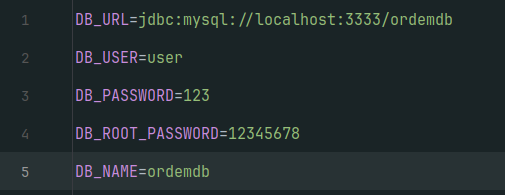
\includegraphics[width=0.5\linewidth]{env_back.png}
    \caption{.env do back-end}
    \label{fig:enter-label}
\end{figure}
        Então vá para o OpApplication e rode a aplicação 
        \begin{figure}[H]
    \centering
    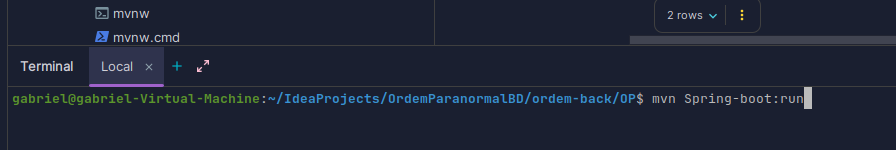
\includegraphics[width=0.5\linewidth]{Screenshot_1.png}
    \caption{Maven RUN}
    \label{fig:enter-label}
\end{figure}
\item \textbf{Front-End:}

Entre na pasta do front:
\begin{lstlisting}
    cd ../ordem-front
\end{lstlisting}

Crie também o .env com o endpoint do back‑end na pasta do front-end:

\begin{lstlisting}
    VITE_API_URL=http://localhost:8080/
\end{lstlisting}

Instale dependências e inicie:

\begin{lstlisting}
    npm install
    npm run dev
\end{lstlisting}

Após isso, abra o navegador em \textbf{http://localhost:5173/} (ou a porta indicada).

Pronto! Com o banco ativo, o back‑end rodando em :8080 e o front‑end em :5173, sua aplicação estará disponível para testes.

\end{enumerate}
    
\chapter{7. Processo do Desenvolvimento}

\subsection{7.1 Definição do Escopo}

O projeto foi concebido para atender às necessidades operacionais da Ordo Realitas, organização secreta dedicada ao enfrentamento de ameaças paranormais. O sistema visa centralizar e organizar o controle de agentes, equipes, missões, ameaças, evidências, rituais e elementos paranormais, respeitando a estrutura hierárquica e os protocolos internos da organização.

\subsection{7.2 Construção do Mini Mundo}

A partir da descrição narrativa da Ordo Realitas, foi elaborado um mini mundo que contempla os principais aspectos da organização: sua liderança centralizada no Veríssimo, os agentes especializados com níveis de exposição (NEX) e patentes, as equipes operacionais com histórico de composição, e o gerenciamento de missões com ameaças classificadas e evidências catalogadas. Elementos adicionais como rituais, elementos paranormais e estrutura dos QGs foram incorporados à lógica do sistema.

\subsection{7.3 Modelagem Conceitual e Lógica}

Com base no mini mundo, foram identificadas as entidades essenciais do sistema e seus relacionamentos. Essa modelagem conceitual foi posteriormente transformada em um modelo lógico relacional, adequado ao uso com banco de dados SQL. Cada entidade foi analisada para garantir a integridade e coerência dos dados, respeitando as regras de negócio do domínio.

\subsection{7.4 Implementação do Banco de Dados}

O banco de dados foi implementado com base no modelo lógico, utilizando o SGBD MySQL. Foram criadas tabelas, chaves primárias e estrangeiras para manter a integridade referencial. A estrutura permite gerenciar desde o cadastro de agentes e equipes até o acompanhamento de missões, ameaças e elementos associados.

\subsection{7.5 Desenvolvimento do Backend}

A camada de backend foi desenvolvida com \textit{Java e Spring Boot}, organizando o projeto em pacotes como controllers, serviços, entidades e DAOs. A comunicação com o banco de dados foi realizada via JDBC Template. As regras de negócio foram implementadas na camada de serviço, respeitando o fluxo de operações descrito no mini mundo. Generalizamos tanto o controller quanto o DAO para conseguir replicar as lógicas de forma simplificada.

\subsection{7.6 Desenvolvimento do Frontend}

O frontend foi construído com \textit{React}, utilizando \textbf{Vite} e \textit{TypeScript}. A aplicação foi organizada em páginas por entidade, com uso de bibliotecas modernas como React Hook Form para formulários e Styled Components para a estilização. Cada entidade possui um serviço HTTP responsável pela comunicação com a API.

\subsection{7.7 Integração}

A integração entre frontend e backend foi feita por meio de chamadas RESTful.

\subsection{7.8 Estilização e Usabilidade}

A interface do sistema foi desenvolvida com foco na clareza e facilidade de uso. A estilização responsiva, feita com Styled Components, proporciona uma navegação fluida, adequada tanto para usuários técnicos quanto operacionais dentro da Ordo Realitas.





%-----------------------------
% REFERÊNCIAS
%-----------------------------
%\newpage
%\addcontentsline{toc}{chapter}{7. Referências}
%\begin{thebibliography}{99}
    %\bibitem{ref1} SOBRENOME, Nome. \textit{Título do livro ou artigo}. Editora, ano.
    %\bibitem{ref2} OUTRO AUTOR. \textit{Outro título}. Local: Editora, ano.
%\end{thebibliography}

\end{document}
